%% USPSC-modelo.tex
% ---------------------------------------------------------------
% USPSC: Modelo de Trabalho Academico (tese de doutorado, dissertacao de
% mestrado e trabalhos monograficos em geral) em conformidade com 
% ABNT NBR 14724:2011: Informacao e documentacao - Trabalhos academicos -
% Apresentacao
%----------------------------------------------------------------
%% Esta é uma customização do abntex2-modelo-trabalho-academico.tex de v-1.9.5 laurocesar 
%% para as Unidades do Campus USP de São Carlos:
%% EESC - Escola de Engenharia de São Carlos
%% IAU - Instituto de Arquitetura e Urbanismo
%% ICMC - Instituto de Ciências Matemáticas e de Computação
%% IFSC - Instituto de Física de São Carlos
%% IQSC - Instituto de Química de São Carlos
%%
%% Este trabalho utiliza a classe USPSC.cls que é mantida pela seguinte equipe:
%% 
%% Programação:
%%   - Marilza Aparecida Rodrigues Tognetti - marilza@sc.usp.br (PUSP-SC)
%%   - Ana Paula Aparecida Calabrez - aninha@sc.usp.br (PUSP-SC)
%% Normalização e Padronização:
%%   - Brianda de Oliveira Ordonho Sigolo - brianda@usp.br (IAU)
%%   - Elena Luzia Palloni Gonçalves - elena@sc.usp.br (EESC)
%%   - Eliana de Cássia Aquareli Cordeiro - eliana@iqsc.usp.br (IQSC)
%%   - Flávia Helena Cassin - cassinp@sc.usp.br (EESC)
%%   - Maria Cristina Cavarette Dziabas - mcdziaba@ifsc.usp.br (IFSC)
%%   - Regina Célia Vidal Medeiros - rcvmat@icmc.usp.br (ICMC)
%%
%% O USPSC-modelo.tex utiliza:	
%%  USPSC.cls e USPSC1.cls
%% 	USPSC-modelo-references.bib
%%	USPSC-modelo.tex
%%	USPSC-unidades.tex
%%	Um dos arquivos com dados pre-textuais abaixo, em conformidade com a Unidade de vínculo do autor:
%%				USPSC-pre-textual-EESC.tex
%%				USPSC-pre-textual-IAU.tex
%%				USPSC-pre-textual-ICMC.tex
%%				USPSC-pre-textual-IFSC.tex
%%				USPSC-pre-textual-IQSC.tex
%%				USPSC-pre-textual-OUTRO.tex
%%	USPSC-fichacatalografica.tex ou fichacatalografica.pdf
%%	folhadeaprovacao.pdf
%%	USPSC-Cap1-Introducao.tex
%%	USPSC-Cap2-Desenvolvimento.tex
%%	USPSC-Cap3-Citacoes.tex
%%	USPSC-Cap4-referencias.tex
%%	USPSC-Cap5-Conclusao.tex
%%	USPSC-Apendices.tex
%%	USPSC-Anexos.tex
%%	USPSC-AcentuacaoLaTeX.tex
%%	USPSC-LetrasGregas.tex
%%	USPSC-SimbolosUteis.tex

%----------------------------------------------------------------
%% Sobre a classe abntex2.cls:
%% abntex2.cls, v-1.9.5 laurocesar
%% Copyright 2012-2015 by abnTeX2 group at https://www.abntex.net.br/ 
%%
%----------------------------------------------------------------

\documentclass[
% -- opções da classe memoir --
12pt,		% tamanho da fonte
openright,	% capítulos começam em pág ímpar (insere página vazia caso preciso)
twoside,  % para impressão em anverso (frente) e verso. Oposto a oneside - Nota: utilizar \imprimirfolhaderosto*
%oneside, % para impressão em páginas separadas (somente anverso) -  Nota: utilizar \imprimirfolhaderosto
% inclua uma % antes do comando twoside e exclua a % antes do oneside 
a4paper,			% tamanho do papel. 
% -- opções da classe abntex2 --
chapter=TITLE,		% títulos de capítulos convertidos em letras maiúsculas
% -- opções do pacote babel --
english,			% idioma adicional para hifenização
french,				% idioma adicional para hifenização
spanish,			% idioma adicional para hifenização
brazil				% o último idioma é o principal do documento
% {USPSC} configura o cabeçalho contendo apenas o número da página
]{USPSC}
%]{USPSC1}
% Inclua % antes de ]{USPSC} e retire a % antes de %]{USPSC1}
% para utilizar o cabeçalho diferenciado para as páginas pares e ímpares como indicado abaixo:
%- páginas ímpares: cabeçalho com seções ou subseções e o número da página
%- páginas pares: cabeçalho com o número da página e o título do capítulo 
% ---

% ---
% Pacotes básicos - Fundamentais 
% ---
\usepackage[T1]{fontenc}		% Seleção de códigos de fonte.
\usepackage[utf8]{inputenc}		% Codificação do documento (conversão automática dos acentos)
\usepackage{lmodern}			% Usa a fonte Latin Modern
% Para utilizar a fonte Times New Roman, inclua uma % no início do comando acima  "\usepackage{lmodern}"
% Abaixo, tire a % antes do comando  \usepackage{times}
%\usepackage{times}		    	% Usa a fonte Times New Roman	
% Lembre-se de alterar a fonte no comando que imprime o preâmbulo no arquivo da Classe USPSC.cls				
\usepackage{lastpage}			% Usado pela Ficha catalográfica
\usepackage{indentfirst}		% Indenta o primeiro parágrafo de cada seção.
\usepackage{color}				% Controle das cores
\usepackage{graphicx}			% Inclusão de gráficos
\usepackage{float} 				% Fixa tabelas e figuras no local exato
%\usepackage{chemfig,chemmacros} % Para escrever reações químicas
\usepackage{microtype} 			% para melhorias de justificação
\usepackage{pdfpages}
\usepackage{makeidx}            % para gerar índice remissimo
% ---

% ---
% Pacotes de citações
% Citações padrão ABNT
% ---
% Sistemas de chamada: autor-data ou numérico.
% Sistema autor-data
\usepackage[alf,abnt-emphasize=bf, abnt-thesis-year=both, abnt-repeated-author-omit=yes, abnt-last-names=abnt, abnt-etal-cite,abnt-etal-list=3, abnt-etal-text=default, abnt-and-type=e, abnt-doi=doi, abnt-url-package=none, abnt-verbatim-entry=no]{abntex2cite}

% Para o IQSC, que indica todos os autores nas referências, incluir % no início do comando acima e retirar a % do comando abaixo 

%\usepackage[alf,abnt-emphasize=bf, abnt-thesis-year=both, abnt-repeated-author-omit=yes, abnt-last-names=abnt, abnt-etal-cite,abnt-etal-list=0, abnt-etal-text=default, abnt-and-type=e]{abntex2cite}

% Sistema Numérico
% Para citações numéricas, sistema adotado pelo IFSC, incluir % no início do comando acima e retirar a % do comando abaixo 
%\usepackage[num,overcite,abnt-emphasize=bf, abnt-thesis-year=both, abnt-repeated-author-omit=yes, abnt-last-names=abnt, abnt-etal-cite,abnt-etal-list=0, abnt-etal-text=default, abnt-and-type=e]{abntex2cite}

% Complementarmente, verifique as instruções abaixo sobre os Pacotes de Nota de rodapé
% ---
% Pacotes de Nota de rodapé
% Configurações de nota de rodapé

% O presente modelo adota o formato numérico para as notas de rodapés quando utiliza o sistema de chamada autor-data para citações e referências. Para utilizar o sistema de chamada numérico para citações e referências, habilitar um dos comandos abaixo.
% Há diversa opções para nota de rodapé no Sistema Numérico.  Para o IFSC, habilitade o comando abaixo.

%\renewcommand{\thefootnote}{\fnsymbol{footnote}}  %Comando para inserção de símbolos em nota de rodapé

% Outras opções para nota de rodapé no Sistema Numérico:
%\renewcommand{\thefootnote}{\alph{footnote}}      %Comando para inserção de letras minúscula em nota de rodapé
%\renewcommand{\thefootnote}{\Alph{footnote}}      %Comando para inserção de letras maiúscula em nota de rodapé
%\renewcommand{\thefootnote}{\roman{footnote}}     %Comando para inserção de números romanos minúsculos  em nota de rodapé
%\renewcommand{\thefootnote}{\Roman{footnote}}     %Comando para inserção de números romanos minúsculos  em nota de rodapé

\renewcommand{\footnotesize}{\small} %Comando para diminuir a fonte das notas de rodapé

 % ---
 % Pacote para agrupar a citação numérica consecutiva
 % Quando for adotado o Sistema Numérico, a exemplo do IFSC, habilite 
 % o pacote cite abaixo retirando a porcentagem antes do comando abaixo
 %\usepackage[superscript]{cite}	

% ---
% Pacotes adicionais, usados apenas no âmbito do Modelo Canônico do abnteX2
% ---
\usepackage{lipsum}				% para geração de dummy text
% ---




% pacotes de tabelas
\usepackage{multicol}	% Suporte a mesclagens em colunas
\usepackage{multirow}	% Suporte a mesclagens em linhas
\usepackage{longtable}	% Tabelas com várias páginas
\usepackage{threeparttablex}    % notas no longtable
\usepackage{array}

%---
% Configurações para o pacote chemfig
%\chemsetup[chemformula]{format=\sffamily}
%\renewcommand*\printatom[1]{\ensuremath{\mathsf{#1}}}
%\setatomsep{2em}
%\setdoublesep{.6ex}
%\setbondstyle{semithick}
%---
% Configurando o ambiente para utilizar os recursos de frases pre-prontas do mhchem
\newenvironment{rslist}%
{%
	\begin{labeling}% environment from KOMA-script
		{\rsnumber{R39/23/24/25}}% R39/23/24/25 is longest label
	}{%
\end{labeling}%
}%
% Definição de comando para utilizar os recursos de frases pre-prontas do mhchem
\newcommand{\rs}[2][]{\item[{\rsnumber[#1]{#2}}] \rsphrase{bb}}
% ---

% ---
% DADOS INICIAIS - Define sigla com título, área de concentração e opção do Programa 
% Consulte a tabela referente aos Programas, áreas e opções de sua unidade contante do
% arquivo USPSC-Siglas estabelecidas para os Programas de Pós-Graduação por Unidade.xlsx 
% ou nos APÊNDICES A-F
\siglaunidade{ICMC-TCC}
\programa{MBACD}
% Os demais dados deverão ser fornecidos no arquivo USPSC-pre-textual-UUUU ou USPSC-TCC-pre-textual-UUUU, onde UUUU é a sigla da Unidade. 
% Exemplo:USPSC-pre-textual-IFSC.tex
% ---
% Configurações de aparência do PDF final
% alterando o aspecto da cor azul
\definecolor{blue}{RGB}{41,5,195}

% informações do PDF
\makeatletter
\hypersetup{
	%pagebackref=true,
	pdftitle={\@title}, 
	pdfauthor={\@author},
	pdfsubject={\imprimirpreambulo},
	pdfcreator={LaTeX with abnTeX2},
	pdfkeywords={abnt}{latex}{abntex}{USPSC}{trabalho acadêmico}, 
	colorlinks=true,       		% false: boxed links; true: colored links
	linkcolor=blue,          	% color of internal links
	citecolor=blue,        		% color of links to bibliography
	filecolor=magenta,      		% color of file links
	urlcolor=blue,
	bookmarksdepth=4
}
\makeatother
% --- 
% --- 
% Espaçamentos entre linhas e parágrafos 
% --- 

% O tamanho do parágrafo é dado por:
\setlength{\parindent}{1.3cm}

% Controle do espaçamento entre um parágrafo e outro:
\setlength{\parskip}{0.2cm}  % tente também \onelineskip

% ---
% compila o sumário e índice
\makeindex
% ---

% ----
% Início do documento
% ----
\begin{document}

% Seleciona o idioma do documento (conforme pacotes do babel)
\selectlanguage{brazil}
% Se o idioma do texto for inglês, inclua uma % antes do 
%      comando \selectlanguage{brazil} e 
%      retire a % antes do comando abaixo
%\selectlanguage{english}

% Retira espaço extra obsoleto entre as frases.
\frenchspacing 

% --- Formatação dos Títulos
\renewcommand{\ABNTEXchapterfontsize}{\fontsize{12}{12}\bfseries}
\renewcommand{\ABNTEXsectionfontsize}{\fontsize{12}{12}\bfseries}
\renewcommand{\ABNTEXsubsectionfontsize}{\fontsize{12}{12}\normalfont}
\renewcommand{\ABNTEXsubsubsectionfontsize}{\fontsize{12}{12}\normalfont}
\renewcommand{\ABNTEXsubsubsubsectionfontsize}{\fontsize{12}{12}\normalfont}


% ----------------------------------------------------------
% ELEMENTOS PRÉ-TEXTUAIS
% ----------------------------------------------------------
% ---
% Capa
% ---
\imprimircapa
% ---
% Folha de rosto
% (o * indica impressão em anverso (frente) e verso )
% ---
\imprimirfolhaderosto*
%\imprimirfolhaderosto
% ---
% ---
% Inserir a ficha catalográfica em pdf
% ---
% A biblioteca da sua Unidade lhe fornecerá um PDF com a ficha
% catalográfica definitiva. 
% Quando estiver com o documento, salve-o como PDF no diretório
% do seu projeto como fichacatalografica.pdf e iclua o arquivo
% utilizando o comando abaixo:
%\includepdf{USPSC-Tese-pre-textual/fichacatalografica.pdf} 
% Se você optar por elaborar a ficha catalográfica, deverá 
% incluir uma % antes da linha % antes
% do comando % ---
% Inserir a ficha bibliografica
% ---
% Isto é um exemplo de Ficha Catalográfica, ou ``Dados internacionais de
% catalogação-na-publicação''. Você pode utilizar este modelo como referência. 
% Porém, provavelmente a biblioteca da sua universidade lhe fornecerá um PDF
% com a ficha catalográfica definitiva após a defesa do trabalho. Quando estiver
% com o documento, salve-o como PDF no diretório do seu projeto e substitua todo
% o conteúdo de implementação deste arquivo pelo comando abaixo:
%
\begin{fichacatalografica}
	\hspace{-1.4cm}
	\imprimirnotaautorizacao \\ \\
	%\sffamily
	\vspace*{\fill}					% Posição vertical
	\begin{center}					% Minipage Centralizado
		\imprimirnotabib \\
\begin{table}[htb]
	\scriptsize
	\centering	
	\begin{tabular}{|p{0.9cm} p{8.7cm}|}
		\hline
	      & \\
		  &	  \imprimirautorficha     \\
		
		 \imprimircutter & 
							\hspace{0.4cm}\imprimirtitulo~  / ~\imprimirautor~ ;  ~\imprimirorientadorcorpoficha. -- 	\imprimirlocal, \imprimirdata.   \\
		
		  &  % Para incluir nota referente à versão corrigida no corpo da ficha,
			  % incluir % no início da linha acima e tirar a % do início da linha abaixo
			  %	\hspace{0.4cm} \imprimirtitulo~  / ~\imprimirautor~ ; ~\imprimirorientadorcorpoficha~- ~\imprimirnotafolharosto. -- \imprimirlocal, \imprimirdata.  \\
		
			\hspace{0.4cm}\pageref{LastPage} p. \\ 
		  & \\
		  & 
		    \hspace{0.4cm}\imprimirnotaficha ~--~ 
						  \imprimirunidademin, 
						  \imprimiruniversidademin, 
		                  \imprimirdata. \\ 
		  & \\                 
		   % Para incluir nota referente à versão corrigida em notas,
		    % incluir uma % no início da linha acima e	
		    % tirar a % do início da linha abaixo
		    % & \hspace{0.4cm}\imprimirnotafolharosto \\ 
		  & \\ 
		  & \hspace{0.4cm}1. classificação de patentes. 2. aprendizado de máquina. 3. processamento de linguagem natural. I. \imprimirorientadorficha. 
		   II. Título. \\
	
		     %Se houver co-orientador, inclua % antes da linha (antes de II. Título.) 
		     %          e tire a % antes do comando abaixo 
		     %III. Título. \\   
		  \hline
	\end{tabular}
\end{table}
	\end{center}
\end{fichacatalografica}
% ---

 
% e retirar o % do comando abaixo
%% ---
% Inserir a ficha bibliografica
% ---
% Isto é um exemplo de Ficha Catalográfica, ou ``Dados internacionais de
% catalogação-na-publicação''. Você pode utilizar este modelo como referência. 
% Porém, provavelmente a biblioteca da sua universidade lhe fornecerá um PDF
% com a ficha catalográfica definitiva após a defesa do trabalho. Quando estiver
% com o documento, salve-o como PDF no diretório do seu projeto e substitua todo
% o conteúdo de implementação deste arquivo pelo comando abaixo:
%
\begin{fichacatalografica}
	\hspace{-1.4cm}
	\imprimirnotaautorizacao \\ \\
	%\sffamily
	\vspace*{\fill}					% Posição vertical
	\begin{center}					% Minipage Centralizado
		\imprimirnotabib \\
\begin{table}[htb]
	\scriptsize
	\centering	
	\begin{tabular}{|p{0.9cm} p{8.7cm}|}
		\hline
	      & \\
		  &	  \imprimirautorficha     \\
		
		 \imprimircutter & 
							\hspace{0.4cm}\imprimirtitulo~  / ~\imprimirautor~ ;  ~\imprimirorientadorcorpoficha. -- 	\imprimirlocal, \imprimirdata.   \\
		
		  &  % Para incluir nota referente à versão corrigida no corpo da ficha,
			  % incluir % no início da linha acima e tirar a % do início da linha abaixo
			  %	\hspace{0.4cm} \imprimirtitulo~  / ~\imprimirautor~ ; ~\imprimirorientadorcorpoficha~- ~\imprimirnotafolharosto. -- \imprimirlocal, \imprimirdata.  \\
		
			\hspace{0.4cm}\pageref{LastPage} p. \\ 
		  & \\
		  & 
		    \hspace{0.4cm}\imprimirnotaficha ~--~ 
						  \imprimirunidademin, 
						  \imprimiruniversidademin, 
		                  \imprimirdata. \\ 
		  & \\                 
		   % Para incluir nota referente à versão corrigida em notas,
		    % incluir uma % no início da linha acima e	
		    % tirar a % do início da linha abaixo
		    % & \hspace{0.4cm}\imprimirnotafolharosto \\ 
		  & \\ 
		  & \hspace{0.4cm}1. classificação de patentes. 2. aprendizado de máquina. 3. processamento de linguagem natural. I. \imprimirorientadorficha. 
		   II. Título. \\
	
		     %Se houver co-orientador, inclua % antes da linha (antes de II. Título.) 
		     %          e tire a % antes do comando abaixo 
		     %III. Título. \\   
		  \hline
	\end{tabular}
\end{table}
	\end{center}
\end{fichacatalografica}
% ---


% As informações que compõem a ficha catalográfica estão 
% definidos no arquivo USPSC-pre-textual-UUUU.tex
% ---


% ---
% ---
% Inserir errata
% ---

%\begin{errata}
%	\OnehalfSpacing 			
%	A errata é um elemento opcional, que consiste de uma lista de erros da obra, precedidos pelas folhas e linhas onde eles ocorrem e seguidos pelas correções correspondentes. Deve ser inserida logo após a folha de rosto e conter a referência do trabalho para facilitar sua identificação, conforme a ABNT NBR 14724 \cite{nbr14724}.
%	
%	Modelo de Errata:
%		
%	\begin{flushleft} 
%			\setlength{\absparsep}{0pt} % ajusta o espaçamento da referência	
%			\SingleSpacing 
%			\imprimirautorabr~ ~\textbf{\imprimirtitulo}.	\imprimirdata. \pageref{LastPage}p. 
%			%Substitua p. por f. quando utilizar oneside em \documentclass
%			%\pageref{LastPage}f.
%			\imprimirtipotrabalho~-~\imprimirinstituicao, \imprimirlocal, \imprimirdata. 
% 	\end{flushleft}
%\vspace{\onelineskip}
%\OnehalfSpacing 
%\center
%\textbf{ERRATA}
%\vspace{\onelineskip}
%\OnehalfSpacing 
%\begin{table}[htb]
%	\center
%	\footnotesize
%	\begin{tabular}{p{1.4cm} p{1cm} p{3cm} p{3cm} }
%		\hline
%		\textbf{Folha} & \textbf{Linha}  & \textbf{Onde se lê}  & \textbf{Leia-se}  \\
%			\hline
%			1 & 10 & auto-conclavo & autoconclavo\\
%		\hline
%	\end{tabular}
%\end{table}
%
%
%\end{errata}
% ---

% ---
% Inserir folha de aprovação
% ---

% A Folha de aprovação é um elemento obrigatório da NBR 4724/2011 (seção 4.2.1.3). 
% Após a defesa/aprovação do trabalho, gere o arquivo folhadeaprovacao.pdf da página assinada pela banca 
% e iclua o arquivo utilizando o comando abaixo:
%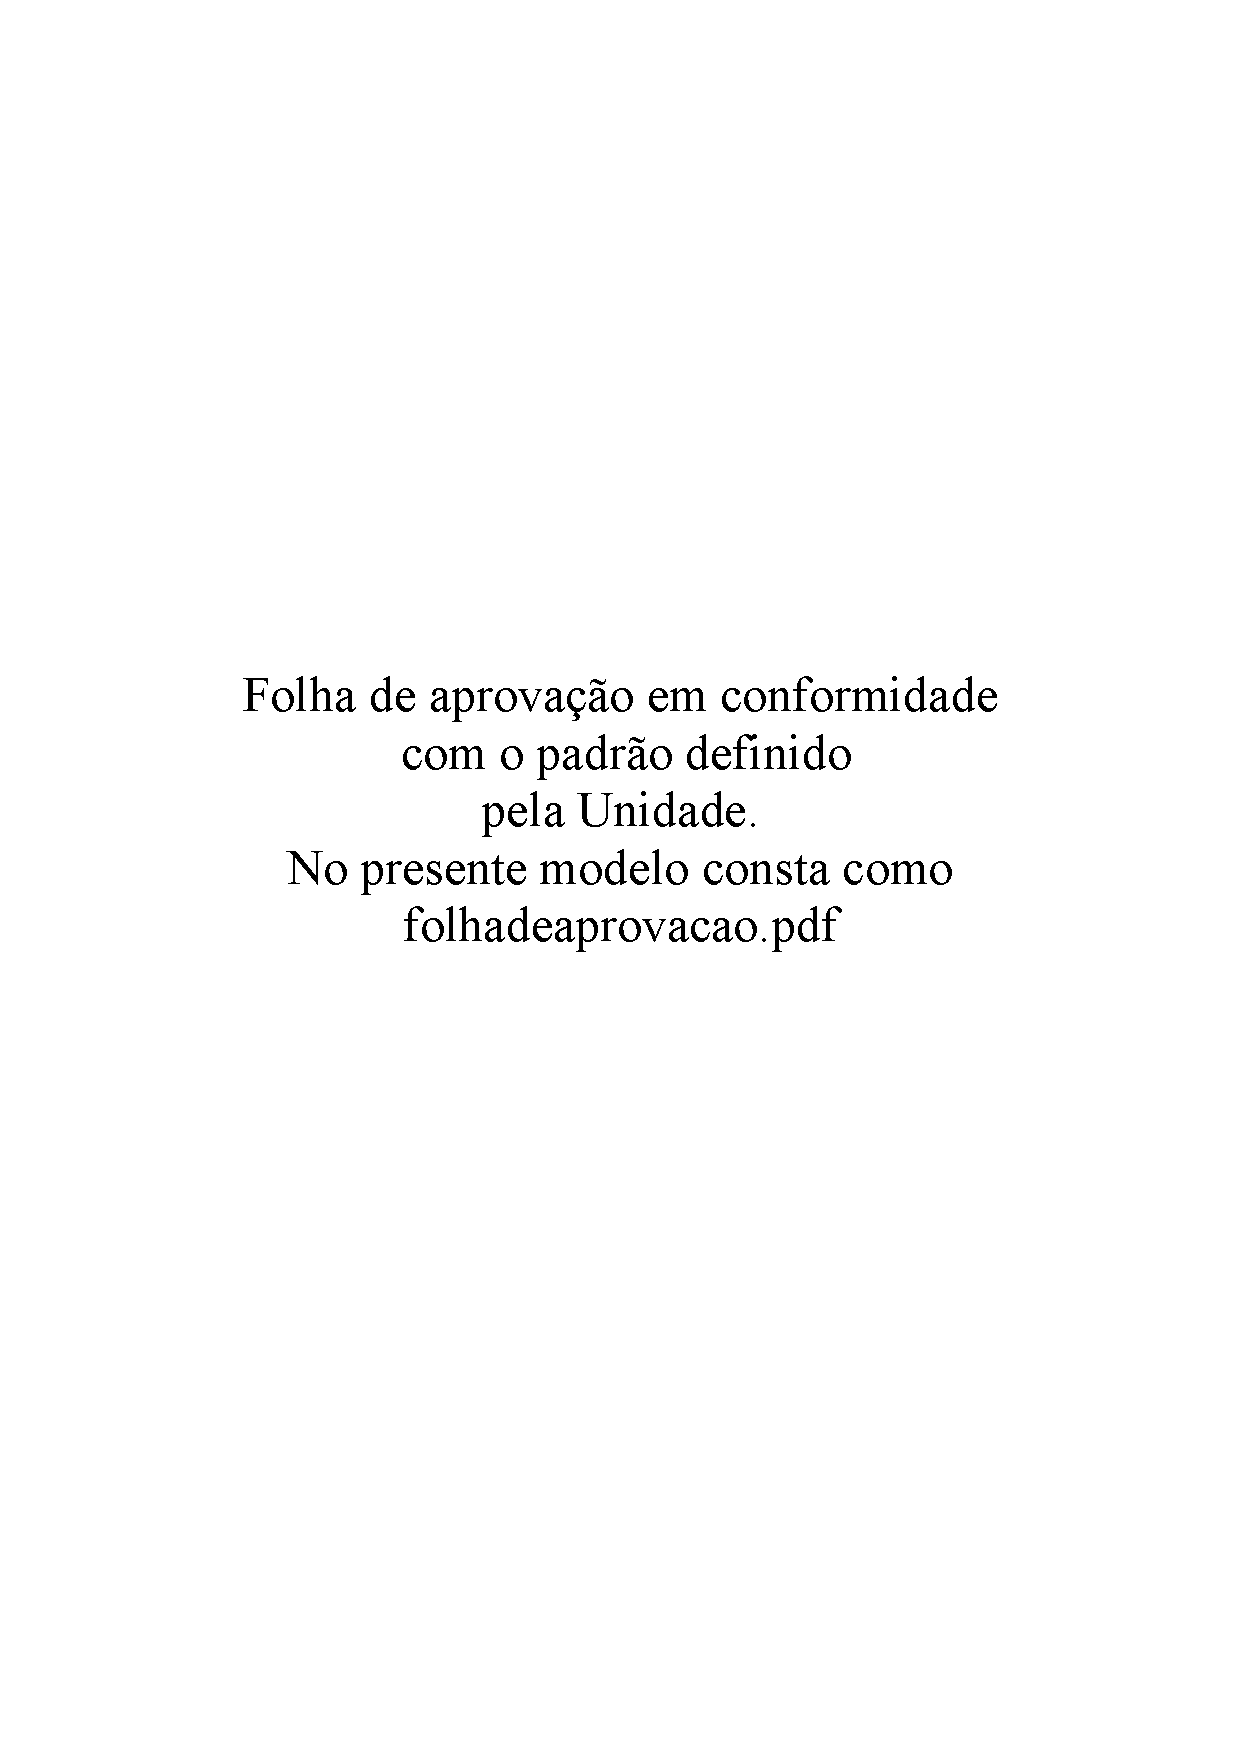
\includepdf{folhadeaprovacao.pdf}
% Alternativa para a Folha de Aprovação:
% Se for a sua opção elaborar uma folha de aprovação, insira uma % antes do comando acima que inclui o arquivo folhadeaprovacao.pdf,
% tire o % do comando abaixo e altere o arquivo folhadeaprovacao.tex conforme suas necessidades
%% Alternativa para a Folha de Aprovação 
% Se esta for a sua opção, exclua inclusão feita acima do arquivo folhadeaprovacao.pdf
%
\begin{folhadeaprovacao}
  \begin{center}
       {\ABNTEXchapterfont\bfseries\large\imprimirautor}
	 \vspace*{2cm}
   
    \begin{center}
      \ABNTEXchapterfont\bfseries\Large\imprimirtitulo
    \end{center}
		\vspace*{2cm}
		\hspace{.45\textwidth}
    \begin{minipage}{.5\textwidth}
        \imprimirpreambulo
    \end{minipage}
		\vspace*{2cm}
    %\vspace*{\fill}
	\end{center}

  \begin{center}
	  {\ABNTEXchapterfont\bfseries\large\ {Data de defesa: 02 de outubro de 2015} \\}
		\vspace*{\fill}
	  {\ABNTEXchapterfont\bfseries\large\ {Comiss\~ao Julgadora:} \\}
		%Trabalho aprovado. \imprimirlocal, 2 de outubro de 2015:
		
		%\assinatura{\textbf{\imprimirorientador} \\ Orientador} 
		\assinatura{\textbf{\imprimirorientador} \\}
    % Se for ORIENTADOR, inclua % no início do comando abaixo e tire a % do próximo comando 
		\renewcommand{\orientadorname}{Orientadora}
		%\renewcommand{\orientadorname}{Orientador}

		\imprimirorientadorRotulo
		\par
		\assinatura{\textbf{Professor} \\ Convidado1}
	
		\assinatura{\textbf{Professor} \\ Convidado2}
		%\assinatura{\textbf{Professor} \\ Convidado3}
		%\assinatura{\textbf{Professor} \\ Convidado4}
		%\begin{center}
		\vspace*{\fill}
   	{\ABNTEXchapterfont\bfseries\large\imprimirlocal}
    \par
    {\ABNTEXchapterfont\bfseries\large\imprimirdata}
\end{center}
\end{folhadeaprovacao}
% ---


\includepdf{PaginaEmBranco.pdf}

% ---
% Dedicatória
% ---
%%% USPSC-Dedicatória.tex
% ---
% Dedicatória
% ---
\begin{dedicatoria}
   \vspace*{\fill}
   \centering
   \noindent
   \textit{ Dedico este trabalho a minha esposa Walkiria e ao meu filho Eduardo.} \vspace*{\fill}
\end{dedicatoria}
% ---
% ---

% ---
% Agradecimentos
% ---
%%% Agradecimentos.tex
% ---
% Agradecimentos
% ---=====
\begin{agradecimentos}
	A motivação para o desenvolvimento da classe USPSC e dos modelos de trabalhos acadêmicos foi decorrente de solicitações de usuários das Bibliotecas do Campus USP de São Carlos. A versão 2.0 do Pacote USPSC é composto da \textbf{Classe USPSC}, do \textbf{Modelo para TCC em \LaTeX\ utilizando a classe USPSC} e do \textbf{Modelo para teses e dissertações em \LaTeX\ utilizando a classe USPSC}.
	
	O Modelo para TCC está disponível inicialmente apenas para EESC e será estendido às demais Unidades de Ensino do Campus USP de São Carlos a medida que as mesmas definirem seus padrões.
	
	O Grupo desenvolvedor do Pacote USPSC agradece especialmente ao Luis Olmes, doutorando do Instituto de Ciências Matemáticas e de Computação (ICMC) da Universidade de São Paulo (USP), pelas primeiras orientações sobre o \LaTeX\ . 
	
	Agradecemos ao Lauro César Araujo pelo desenvolvimento da classe  \abnTeX, modelos canônicos e tantas outras contribuições que nos permitiu o desenvolvimento da classe USPSC e seus modelos.
	
	Os nossos agradecimentos aos integrantes do primeiro
	projeto abn\TeX\, Gerald Weber, Miguel Frasson, Leslie H. Watter, Bruno Parente Lima, Flávio de Vasconcellos Corrêa, Otavio Real
	Salvador, Renato Machnievscz, e a todos que contribuíram para que a produção de trabalhos acadêmicos em conformidade com
	as normas ABNT com \LaTeX\ fosse possível.
	
	Agradecemos ao grupo de usuários
	\emph{latex-br}{\url{http://groups.google.com/group/latex-br}}, aos integrantes do grupo
	\emph{\abnTeX}{\url{http://groups.google.com/group/abntex2}  e \url{http://www.abntex.net.br/}}~que contribuem para a evolução do \abnTeX.
\end{agradecimentos}
% ---
% ---

% ---
% Epígrafe
% ---
\begin{epigrafe}
    \vspace*{\fill}
	\begin{flushright}
		\textit{``Nenhuma grande descoberta foi feita jamais sem um \\
		palpite ousado.''\\
		Isaac Newton}
	\end{flushright}
\end{epigrafe}
% ---

% A T E N Ç Ã O
% Se o idioma do texto for em inglês, o abstract deve preceder o resumo
% resumo em português
%
% Resumo
% ---
%%% Resumo.tex
% ---
% Resumo
% ---
\setlength{\absparsep}{18pt} % ajusta o espaçamento dos parágrafos do resumo		
\begin{resumo}
	\begin{flushleft} 
			\setlength{\absparsep}{0pt} % ajusta o espaçamento da referência	
			\SingleSpacing 
			\imprimirautorabr~ ~\textbf{\imprimirtitulo}.	\imprimirdata. \pageref{LastPage}p. 
			%Substitua p. por f. quando utilizar oneside em \documentclass
			%\pageref{LastPage}f.
			\imprimirtipotrabalho~-~\imprimirinstituicao, \imprimirlocal, \imprimirdata. 
 	\end{flushleft}
\OnehalfSpacing 			
Os documentos de patentes são largamente utilizados por empresas para a construção estratégias de produção, \textit{marketing} e desenvolvimento. O tempo gasto em pesquisa é influenciado pela quantidade de patentes em que os pesquisadores deverão ler e estudar para gerar algum \textit{insight} significativo. Neste trabalho nos propomos a desenvolver uma metodologia de classificação de documentos de patentes por áreas de interesse facilitando o encontro de patentes mais relevantes. Faremos uso de técnicas de processamento de linguagem natural e compararemos os modelos mais utilizados na classificação de textos.
 

 \textbf{Palavras-chave}: Classificação, Documento de patente, corpora, RandomForest, SVM, Naive Bayes, Dicionário, Processamento de Linguagem Natural, TF-IDF, Latent Dirichlet Allocation
\end{resumo}
% ---

% Abstract
% ---
%%% Abstract.tex
% ---
% Abstract
% ---
\autor{Silva, M. J.}
\begin{resumo}[Abstract]
 \begin{otherlanguage*}{english}
	\begin{flushleft} 
		\setlength{\absparsep}{0pt} % ajusta o espaçamento dos parágrafos do resumo		
 		\SingleSpacing 
 		\imprimirautorabr~ ~\textbf{\imprimirtitleabstract}.	\imprimirdata.  \pageref{LastPage}p. 
		%Substitua p. por f. quando utilizar oneside em \documentclass
		%\pageref{LastPage}f.
		\imprimirtipotrabalho~-~\imprimirinstituicao, \imprimirlocal, 	\imprimirdata. 
 	\end{flushleft}
	\OnehalfSpacing 
   Patent documents are widely used by companies to build production, marketing and development strategies. The time spent on research is influenced by the number of patents that researchers must read and study to generate some meaningful insight. In this work we propose to develop a methodology for classifying patent documents by areas of interest, facilitating the finding of more relevant patents. We will make use of natural language processing techniques and compare the most used models in the classification of texts.

   \vspace{\onelineskip}
 
   \noindent 
   \textbf{Keywords}: Classification, Patent Document, corpora, RandomForest, SVM, Naive Bayes, Dictionary, Natural Language Processing, TF-IDF, Latent Dirichlet Allocation
 \end{otherlanguage*}
\end{resumo}

% ---

% ---
% inserir lista de figuras
% ---
%\pdfbookmark[0]{\listfigurename}{lof}
%\listoffigures*
%\cleardoublepage
% ---

% ---
% inserir lista de tabelas
% ---
%\pdfbookmark[0]{\listtablename}{lot}
%\listoftables*
%\cleardoublepage
% ---

% ---
% inserir lista de quadros
% ---
%\pdfbookmark[0]{\listofquadroname}{loq}
%\listofquadro*
%\cleardoublepage
% ---

% ---
% inserir lista de abreviaturas e siglas
% ---
\begin{siglas}
	\item[IDE] Integrated Development Environment
    \item[SVM] Support Vector Machine
    \item[TF-IDF] Term Frequency - Inverse Document Frequency
    \item[FPO] Free Patents Online
    \item[DTM] Document-Term Matrix
    \item[LDA] Latent Dirichlet allocation
	
\end{siglas}
% ---

% ---
% inserir lista de símbolos
% ---
%\begin{simbolos}
%  \item[$ \Gamma $] Letra grega Gama
%  \item[$ \Lambda $] Lambda
%  \item[$ \zeta $] Letra grega minúscula zeta
%  \item[$ \in $] Pertence
%\end{simbolos}
% ---
% ---
% inserir o sumario
% ---
\pdfbookmark[0]{\contentsname}{toc}
\tableofcontents*
\cleardoublepage
% ---
% ----------------------------------------------------------
% ELEMENTOS TEXTUAIS
% ----------------------------------------------------------
\textual
% Os capítulos são inseridos como arquivos externos 

% Capítulo 1 - Introdução
% ---
%% USPSC-Introducao.tex

% ----------------------------------------------------------
% Introdução (exemplo de capítulo sem numeração, mas presente no Sumário)
% ----------------------------------------------------------
\chapter[Introdução]{Introdução}


\section{Apresentação}	

No desenvolvimento geral de produtos, a pesquisa por documentos de patentes visa garantir o não infringimento de propriedades intelectuais que ainda não estão em domínio público \cite{Breitzman2002}.  O sistema de patentes é um conjunto de medidas utilizados para visar o retorno do valor privado investido ao valor social de suas invenções, fornece aos inventores um período temporário de poder de mercado, recuperando os custos de seus investimentos na pesquisa \cite{Williams2017}. De acordo com o \textit{World Intellectual Property Indicator 2017}, em 2016, o número de documentos de patente excedeu 3 milhões pela primeira vez, um aumento de 8.3\% \cite{Li2018}. Em uma pesquisa de documentos de patente, documentos relacionados a tecnologia, economia e jurídico são tratadas, classificadas e analisadas para se obter uma grande vantagem técnica e comercial \cite{Li2018}.

A classificação de documentos é o processo de classificação de um documento em uma ou mais categorias predefinidas, desempenhando um papel importante no gerenciamento e busca de temas \cite{Anne2017}. A automatização da classificação de documentos a partir do uso de aprendizado de máquina, pode rotular documentos a um tema único, mas a rotulagem em dois ou mais temas ainda é relativamente um problema desafiador \cite{Anne2017}.

De acordo com Shahid et al (2020), a classificação de documentos de patente em temas e a atribuição de valor de relevância para estes temas, permitem ao pesquisador filtrar as patentes que o interessa e reduzindo o escopo de análise. Nesse trabalho, realizou-se a construção de uma matriz de valores de \textit{term frequency - inverse document frequency} (TF-IDF), notações e peso ponderado por BestMatch25 (BM25), que posteriormente foi testado em diferentes classificadores, classificando os documentos de patente em cada assunto.
Vide Anne et al (2017), identificou uma matriz de métodos a serem aplicados com os modelos k-Nearest Neighbors (kNN),  Support Vector Machine (SVM), Random Forest e J48. Os principais passos para essa pesquisa foram técnicas de seleção de características, com uso de ganho de informação e correlação para efetividade do classificadores.

Destes dois estudos, foi observado que a adição de mais características para os modelos de classificação utilizados, a acurácia foi melhorada \cite{shahid2020}. E que obstáculos, como o desbalanceamento dos dados foram atenuados pela adição de novas características \cite{Anne2017}. Balancear a relação entre esses dois pontos é um desafio quanto a classificação de documentos de patente.

\section{Justificativa}
Como tratar, classificar e analisar documentos de patente havendo algumas centenas de documentos sobre um assunto específico? O método tradicional necessita de tempo e equipe para realizá-lo, apresentando um resultado com deficiências devido ao alto volume de documentos de patente a serem analisadas \cite{Li2018}. Hoje, já há portais web que oferecem ferramentas das quais algumas auxiliam ao pesquisador a reduzir essa pesquisa \cite{Abbas2014}, mas classificam os documentos em uma relevância geral. Esse resultado somente demonstra que dentro daquela amostra de documentos, uma visão macro sobre o tema que muitas vezes o pesquisador está em busca de um subtema, como quais mercados essa tecnologia está presente, quais os processos de produção desta tecnologia ou qual a formulação desse composto. 

\section{Problema}
Com o rápido crescimento de documentos de patente, torna-se urgente a questão de automatização da classificação de documentos de patente de forma acurada e rápida \cite{Zhu2020}. Os documentos de patente contêm um potencial conhecimento tecnológico na resolução de problemas no processo de fabricação, nos quais são de grande valor científico e tecnológico, no entanto, esse conhecimento está implícito em longos textos \cite{Li2018, Wang2016}. A classificação de documentos de patente em temas e subtemas utilizando de modelos de aprendizado  de máquina se beneficiaria do uso da extração de características uteis vindas do próprio documento \cite{Anne2017}. Observa-se que mais de 90\% das informações de científicas e tecnológicas estão em documentos de patente, e sua análise resultaria em decisões de negócio de sucesso \cite{Li2018}.

\section{Objetivo geral}
Este projeto se propõe a classificar documentos de patente por tema específico e subtemas de interesse do pesquisador, reduzindo o escopo de documentos de patentes a serem estudados à somente os mais relevantes para o que se procura.

\section{Objetivos específicos}
A classificação de documentos de patente envolverá o uso de técnicas de processamento de linguagem natural para o tratamento e preparação dos dados que serão usados no modelo de classificação por relevância que será desenvolvido. Este modelo usará inicialmente a medida estatística TF-IDF e avaliaremos outras medidas. Haverá a necessidade de criação de dicionários que auxiliem na classificação dos documentos de patente. E então será treinado um algoritmo para classificar os documentos de acordo com o tema. 

\section{Metodologia}
Realizaremos a obtenção de um conjunto de documentos de patente aplicado a agricultura através da ferramenta \textit{Free Patents Online} - FPO (https://www.freepatentsonline.com/). Não foi encontrado artigos ou materiais que fizessem essa aplicação para patentes relacionadas ao setor agronômico, para gerenciamento de patentes, desenvolvimento de produtos e descoberta de mercados. 
Faremos o uso do modelo de classificação baseado em florestas aleatórias, a vantagem desse modelo, é a flexibilidade para o uso em regressão e classificação, além da sua facilidade de interpretação do resultado obtido.  
A construção de dicionários será a partir de técnicas de Processamento de Linguagem Natural, elencando as palavras mais relacionadas a área. A analise, construção de dicionários e modelagem do modelos de regressão e classificação será feita na linguagem de programação Python.

% ---

% ---
% Capítulo 2
% ---
%% USPSC-Cap2-Desenvolvimento.tex 

% ---
% Este capítulo, utilizado por diferentes exemplos do abnTeX2, ilustra o uso de
% comandos do abnTeX2 e de LaTeX.
% ---

\chapter{Desenvolvimento}\label{cap_exemplos}

\section{Revisão sistemática}
O estudo de Revisão Sistemática da Literatura seguiu as recomendações \textit{Preferred Reporting Items for Systematic Reviews and Meta-Analisys} – PRISMA.
Foram buscados os termos: “\textit{patent mining}”, “\textit{patent}”, “\textit{random forest}”, “\textit{machine learning}” - nas seguintes bases de dados: Periodicos CAPES, \textit{Microsoft research}, \textit{Semantic Scholar} e \textit{Google Scholar}. O intervalo de publicação dos artigos selecionados estão entre 2012 a 2020 e restrito a somente artigos escritos em inglês.

\subsection{Descrição do objeto de estudo}
Foi realizada a extração de dados de documentos de patentes no site \textit{Free Patents Online} - FPO (https://www.freepatentsonline.com/). Este site contem os dados dos documentos de patentes de forma pública.

\subsection{Delineamento da pequisa}
Foi buscado o termo “\textit{agronomy}” e filtrado para somente documentos de patentes registrados nos Estados Unidos. Foi totalizado 12906 patentes, dos quais selecionamos uma amostragem das 200 primeiras patentes. Construímos uma aplicação de \textit{webscraping} na linguagem Python para realizar a extração dos dados de documentos de patentes.  Os dados extraídos foram armazenados em um banco de dados.

\section{Materiais e métodos}

\subsection{Extração dos dados}
A aplicação de \textit{webscraping} dos dados de documentos de patentes foi escrita na linguagem de programação Python, com uso das bibliotecas \textit{requests} e \textit{BeautifulSoup}. Essa aplicação é modular o suficiente para que seja definido quantos documentos de patentes terão suas informações extraídas, como também quais informações serão extraídas, como demonstrado na Figura \ref{webscraping_flow_image}. Os dados são organizados na forma de tabela e armazenado em um pequeno banco de dados feito em \textit{SQLite}.

\begin{figure}[ht!]
	\centering
	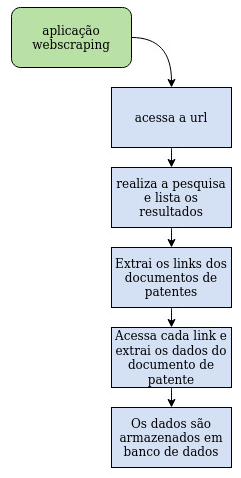
\includegraphics[scale=0.5]{imagens/tcc_webscraping.jpg}
	\caption{Fluxo de captura dos dados de documentos de patente 
			 \label{webscraping_flow_image}}
\end{figure}


\subsection{Construção do dicionário}
A construção do dicionário utilizado no projeto é composta pelas seguintes etapas, Figura \ref{dicionario_flow_image}, geração de um corpora de documentos de patentes, pre processamento do corpora, obtenção da matriz de documento-termo (\textit{Document-Term Matrix} – DTM) e aplicação do modelo \textit{Latent Dirichlet allocation} (LDA). A partir dos tópicos apresentados pelo resultado do LDA, são adicionados aos tópicos, palavras relacionadas, tais como sinônimos, hiperônimos e hipônimos através do banco de dados \textit{wordnet}.

\begin{figure}[ht!]
	\centering
	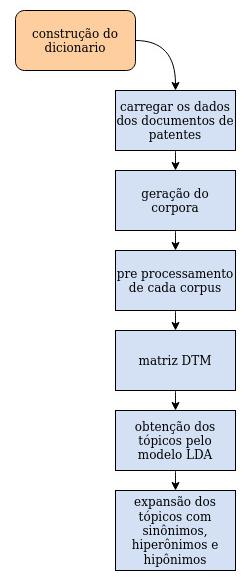
\includegraphics[scale=0.5]{imagens/tcc_dicionario.jpg}
	\caption{Fluxo de criação do dicionário.
			 \label{dicionario_flow_image}}
\end{figure}

\subsection{Validação do dicionário}
A avaliação do dicionário obtido, consiste em observar se o valor k utilizado para geração de tópicos conseguiu separar adequadamente os assuntos contidos no corpora.

\subsection{Classificação a partir do dicionário}
Esta etapa consiste em utilizar o dicionário para classificar os documentos de patentes a partir da iteração com cada termo do dicionario para o conjunto de termos de cada documento, classificando para cada tópico. Esta tarefa é demorada e o tempo necessário aumenta exponencialmente conforme aumenta o tamanho do corpora utilizado. A base de dados gerada será usada para ensinar ao modelo como classificar novos documentos de patentes.


\subsection{Modelagem}
Utilizaremos três dos modelos mais citados na classificação de texto, o \textit{RandomForest}, \textit{Naive Bayes} e \textit{SVM} para avaliar qual se adéqua melhor a essa classificação. Usaremos as técnicas de pré processamento para garantir que o mesmo dado será testado igualmente para cada modelo e escolheremos o modelo de melhor acurácia como modelo final.


\section{Resultados}

\subsection{Extração de dados}

Extraímos uma amostra no total de 904 documentos de patentes através do uso da técnica de \textit{webscraping}. Destes documentos, os dados de \textbf{Titulo} e \textbf{Resumo} foram pré processados, removendo as quebras de linhas, espaços no inicio e fim da frase, uso de somente um espaço como separador e transformação do texto em minúsculo. Estes dados foram concatenados e usados para a montagem do corpora de documentos de patentes, que poderá ser utilizado para outros projetos. Podemos visualizar na Figura \ref{wordcloud_pre_image} como é distribuida a relação de palavras.

\begin{figure}[ht!]
	\centering
	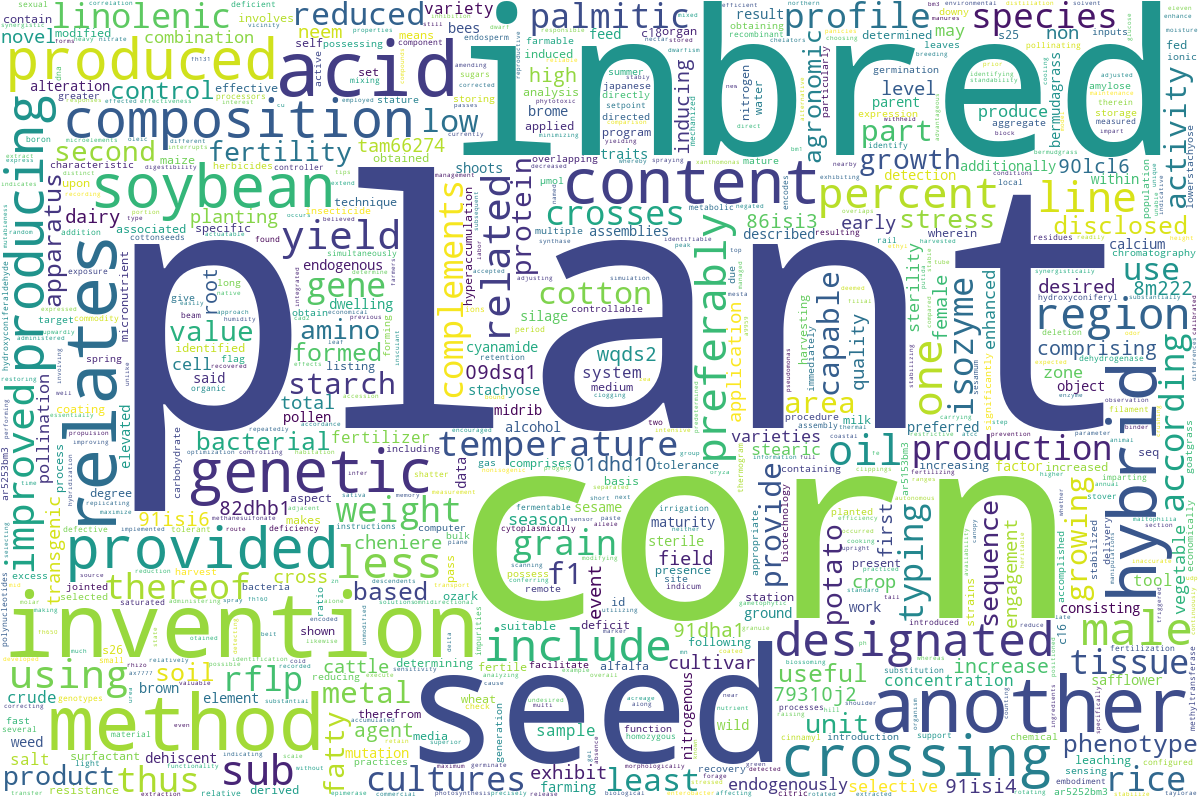
\includegraphics[scale=0.3]{imagens/wordcloud_preprocess.png}
	\caption{Construção nuvem de palavras dos termos mais representativos para este corpora.
			 \label{wordcloud_pre_image}}
\end{figure}

\subsection{Construção do dicionário}

A construção do dicionário engloba o levantamento de tópicos, validação dos tópicos e a expansão do dicionário.

\subsubsection{Levantamento de tópicos}

Foi utilizado o corpora de documentos de patentes feito no passo anterior, onde foi removido as \textbf{\textit{stopwords}} (palavras que não possuem importância a frase, por exemplo em Inglês: \textit{The}, \textit{from}, \textit{a}, \textit{an}, \textit{with}, etc.), foram removidos também caracteres numéricos e especiais. O conteúdo de cada corpus foi separado em uma lista palavras, este processo denomina-se como geração de \textbf{\textit{tokens}} e cada \textit{token} foi desflexionado para a sua palavra raiz (\textbf{\textit{lemmas}}). Obtivemos 904 conjuntos de palavras normalizadas, representando cada documento de patente e que está pronto para ser utilizado em modelos de Processamento de Linguagem Natural e em modelos de Aprendizado de Máquina.
Aplicamos o \textbf{modelo LDA}, com os seguintes parâmetros - \textit{random\_state} igual a 100, \textit{update\_every} igual a 1, \textit{chuncksize} igual a 100, passes igual a 10 e \textit{alpha} automático. Para definir a quantidade de tópicos k, usamos um laço de 40 interações e anotamos o valor da métrica Coherence.

\begin{figure}[ht!]
	\centering
	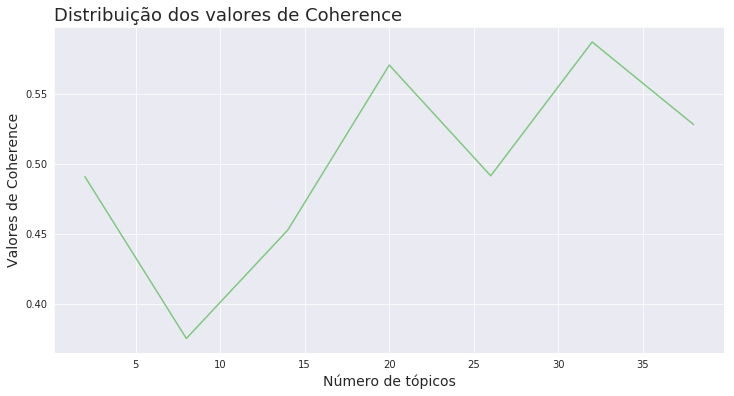
\includegraphics[scale=0.6]{imagens/distr_dos_valores_de_coherence.png}
	\caption{A distribuição dos valores de Coherence ao longo da variação do \textbf{parâmetro k}, permite que observemos qual a quantidade de tópicos mais relevantes a se utilizar.
			 \label{dist_coherence_image}}
\end{figure}

O gráfico da Figura \ref{dist_coherence_image} aponta que um k igual a 25 resulta no mais alto valor de Coherence. Utilizaremos este valor para k para se definir os títulos de tópico.

\subsubsection{Validação dos tópicos}

Examinamos os tópicos obtidos através da ferramenta pyLDAvis, Figura \ref{pyLDAvis_image}. Os termos que compõem os tópicos gerados  representam bem o corpora usado. Temos pouca sobreposição, com exceção do tópico 18, e os termos de cada tópico possuem uma alta relevância com o tema agronomia.  

\begin{figure}[ht!]
	\centering
	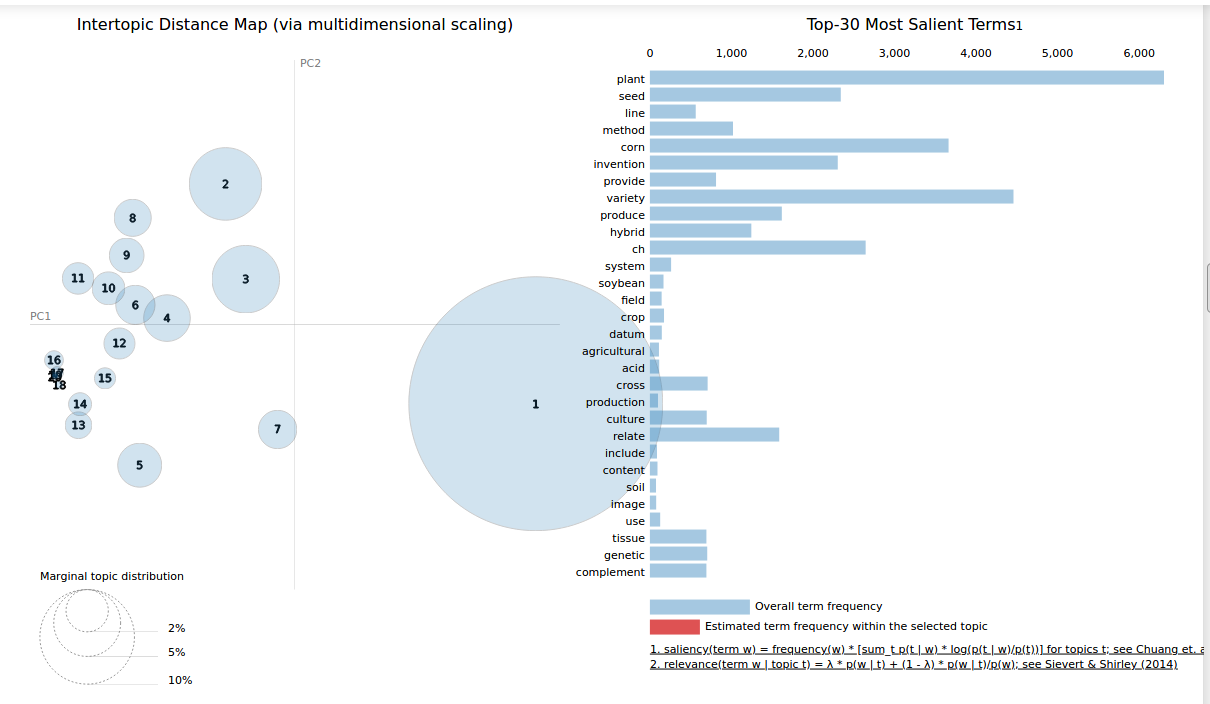
\includegraphics[scale=0.4]{imagens/construcao_dicionario.png}
	\caption{O grafico de bolhas, cada bolha representa um tópico, o tamanho da bolha representa a prevalencia do tópico e a sobreposição de bolhas aponta a similaridade entre os tópicos. O gráfico da direita, as barras representam a relevância do termo para o tópico observado.
			 \label{pyLDAvis_image}}
\end{figure}

\subsubsection{Expansão do dicionário}

Antes de expandir o dicionário, realizamos a remoção de dois tópicos que estavam muito similares. Os tópicos geraram no total de 144 termos únicos que foram submetidas ao \textit{wordnet} e adicionado os sinônimos, hiperônimos e hipônimos destes termos, totalizando 616 termos que representam cada tópico. A estrutura do dicionário criado é composta por três colunas, a primeira é o tópico, a segunda são os termos que estão atrelada ao tópico e a terceira coluna são as palavras derivadas dos termos.

Obtivemos no final um dicionário com com 901 linhas e três colunas, que foi utilizado para fazer uma classificação inicial dos documentos de patentes. 

\subsubsection{Construção da base de dados}

A base de dados composta a partir das informações de identificação documento de patente, o título do documento de patente e o seu resumo. A partir do dicionario fizemos uma classificação, onde atribuímos a cada documento de patente os tópicos a que se referem. A estrutura da base de dados é de 817 linhas e 7 colunas, sendo que 87 linhas foram removidas por não conterem título ou resumo.

\subsubsection{Construção do modelo}

Para a construção do modelo principal, os seguintes modelos foram testados, Random Forest, Naive Bayes e SVM, os principais modelos aplicados em classificação de texto. O seguinte fluxo de analise de dados foi aplicado:

\paragraph{Pre processamento}

\subparagraph{Matriz documento-termo}

Conversão da tabela de entrada em uma matriz documento-termo, esta matriz tem a estrutura da seguinte forma:

\begin{itemize}
  \item colunas: palavras de relevância
  \item linhas: documentos
  \item valores: correspondem ao valor de TF-IDF obtido, quando a palavra não consta na entrada, o valor será igual a zero.
\end{itemize}

A matriz resultante possui 817 linhas e 3492 colunas.
	
\subparagraph{Remoção de stopwords}

Ao converter a tabela de entrada em uma matriz de documento-termo, as colunas são todas palavras de todos os documentos de patente, fazendo-se necessário a remoção de stop-words, resultando em uma tabela com 817 linhas e 3402 colunas.

\subparagraph{Seleção de características}

A seleção de características tem como objetivo selecionar as colunas que possuam maior relevância a coluna alvo. Utilizamos o método RFE para reduzir o numero de colunas para somente 20. Nossa matriz final possui 817 linhas por 20 colunas.

\subparagraph{Modelo}

Os seguintes parâmetros foram utilizados para cada modelo, seguido do valor de acurácia obtido:
	
\begin{itemize}
  \item RandomForest
  \begin{itemize}
    \item critério de separação: Gini
    \item profundidade máxima: 5
    \item validação cruzada de 10 folds
    \item \textbf{acurácia igual a $0.83$}
  \end{itemize}
  \item NaiveBayes
  \begin{itemize}
    \item foram mantidos o valor padrão para cada parâmetro
    \item \textbf{acurácia igual a $0.80$}
  \end{itemize}
  \item SVM
  \begin{itemize}
    \item custo: 1,5
    \item \textbf{acurácia igual a $0.78$}
  \end{itemize}
\end{itemize}	

\subparagraph{Avaliação de parametros}
	
O modelo escolhido foi o RandomForest por ter o maior valor de acurácia, avaliamos se os parâmetros de profundidade máxima poderia ser melhorado como visto na figura \ref{validation_curve_max_depth_rf}.

\begin{figure}[ht!]
	\centering
	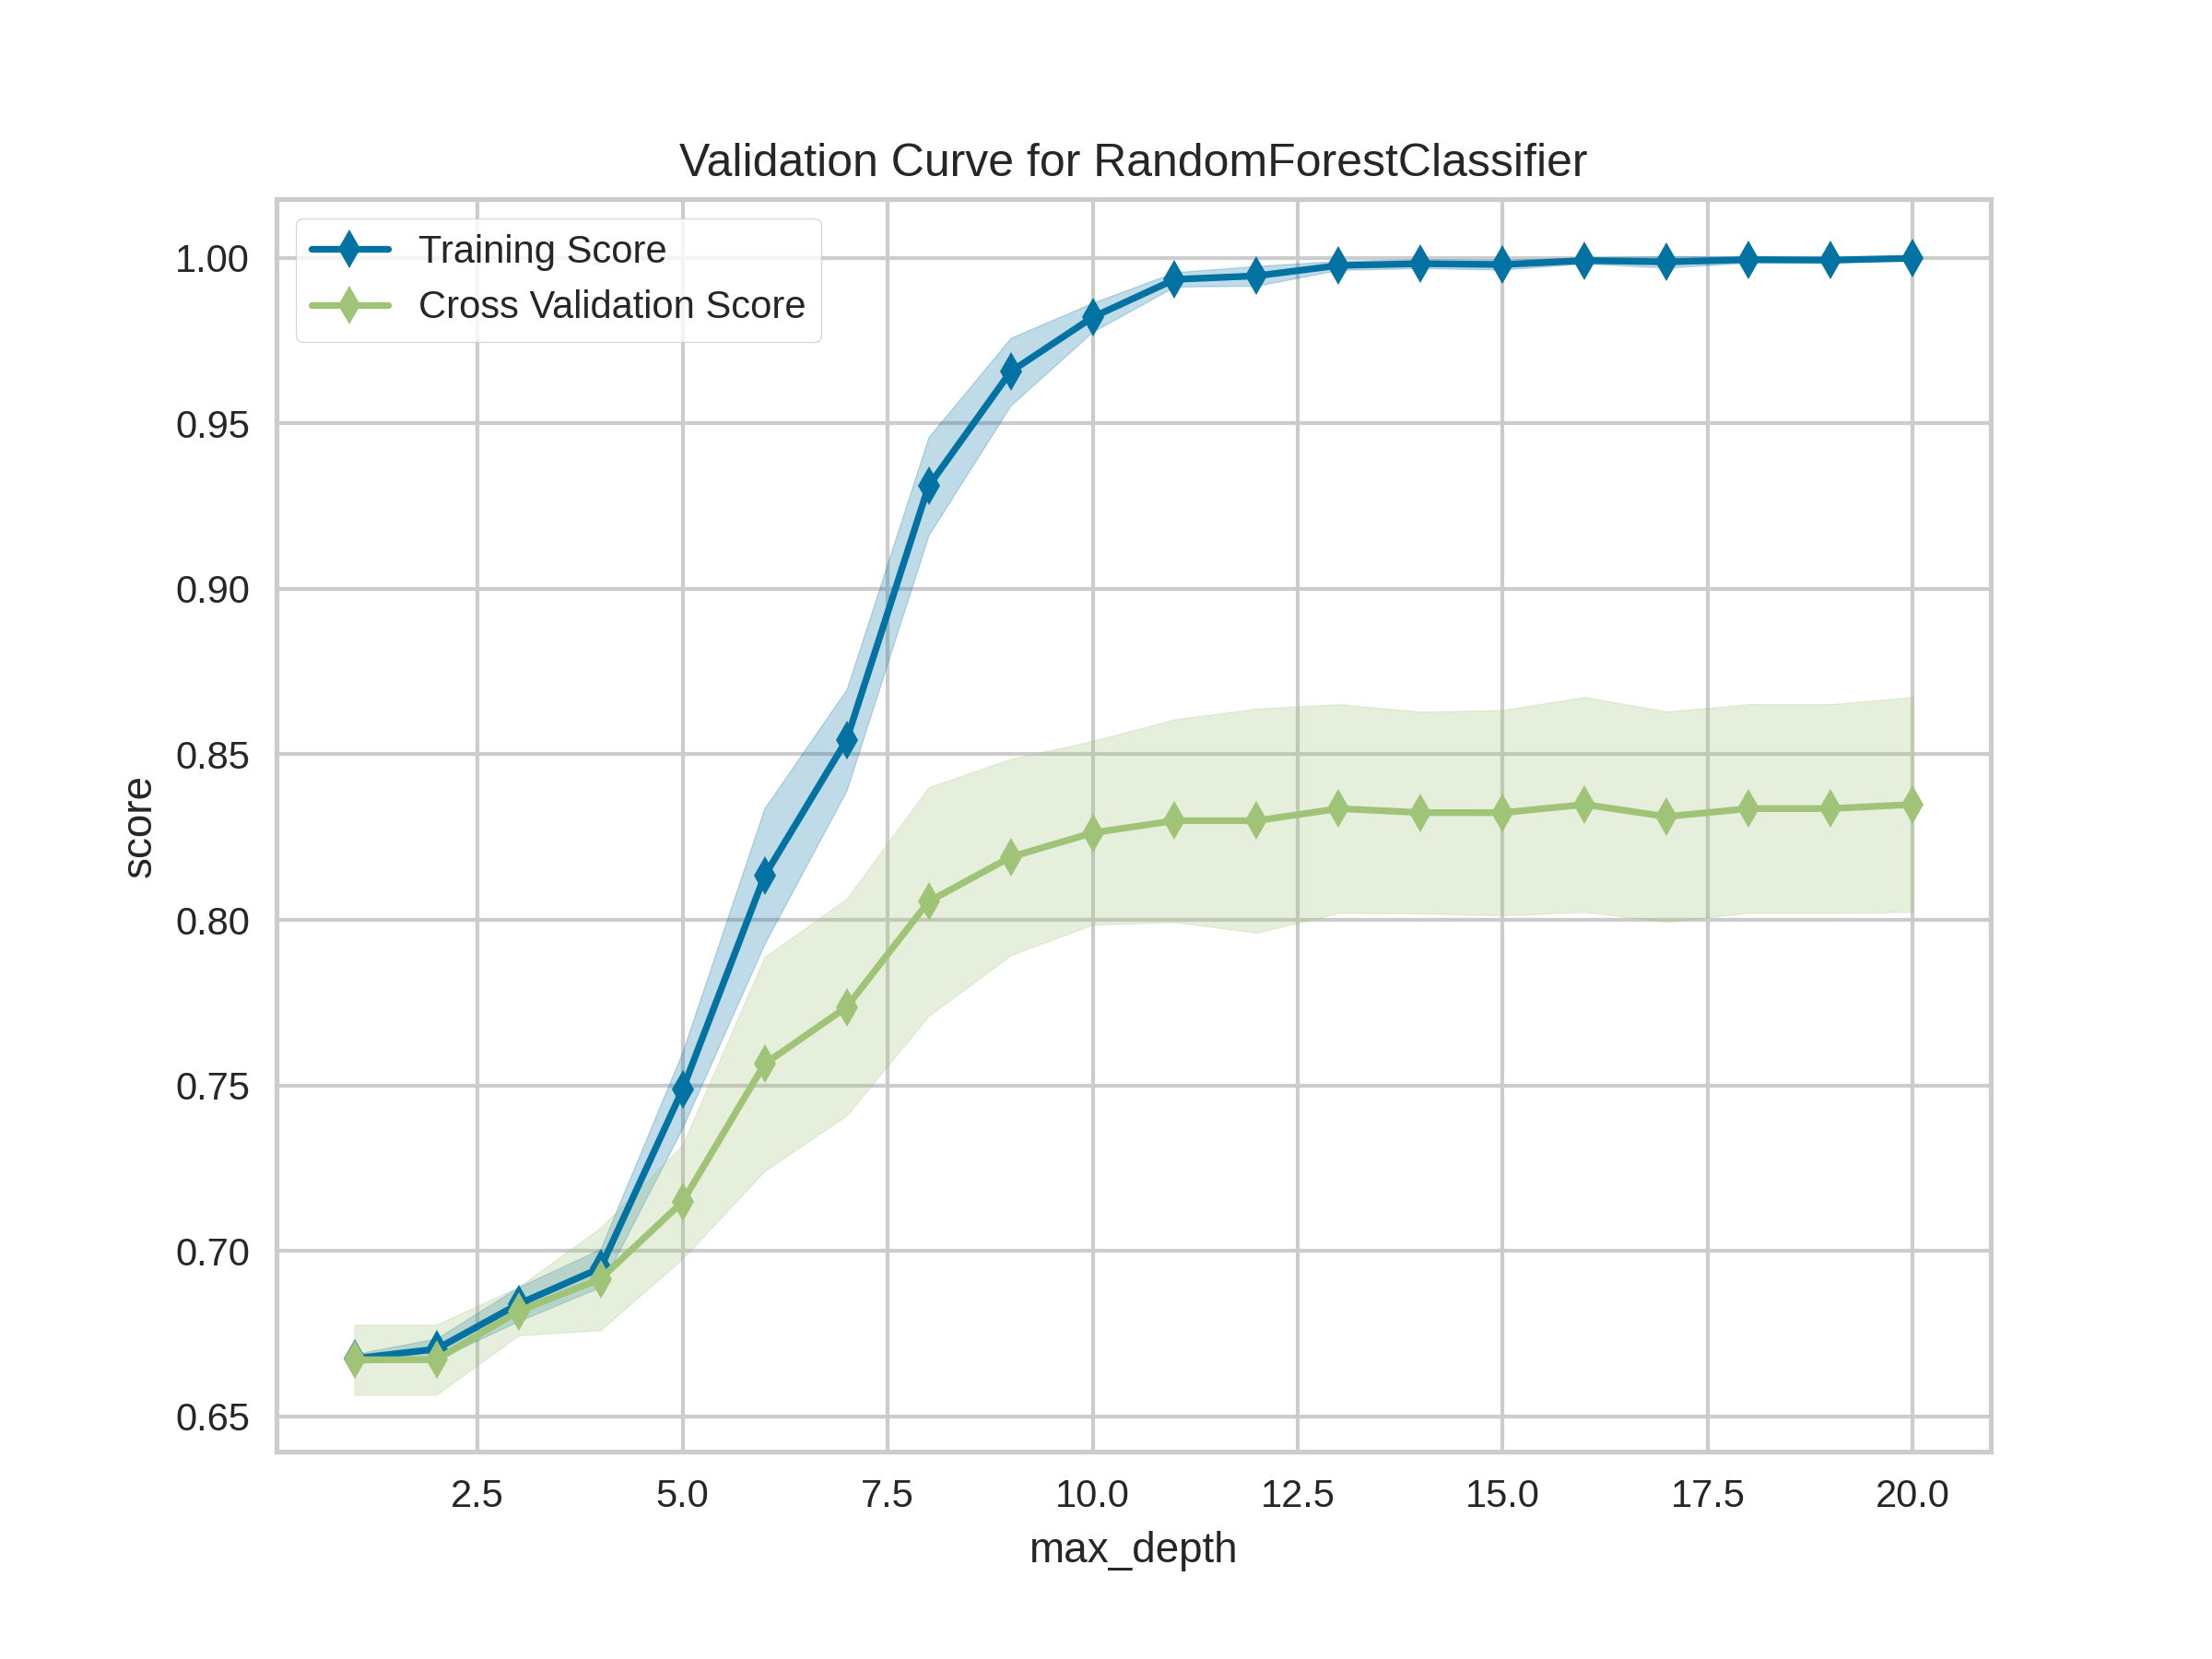
\includegraphics[scale=0.8]{imagens/validation_curve_max_depth_rf.png}
	\caption{Plot do valor de acurácia obtido para cara valor de profundidade máxima. Podemos observar que para os dados de treino e validação se estabiliza após o valor 10.
			 \label{validation_curve_max_depth_rf}}
\end{figure}

Após ajustar o parâmetro de máxima profundidade para 15, obtivemos uma acurácia de 0,84. Não houve um ganho significativo em alterar o parâmetro de máxima profundidade.

\section{Discussão}

Conseguimos realizar a extração bem sucedida de uma amostra de documentos de patentes, do qual pré processamos e criamos um corpora que poderá ser usado não somente para este trabalho como para outros trabalhos com documentos de patentes sobre o tema de agronomia. Fizemos um primeiro levantamento dos tópicos usando o modelo LDA e obtivemos 25 tópicos que serão avaliados e rotulados corretamente. 
Utilizando termos simples para rotular os tópicos neste primeiro momento percebemos que dois tópicos puderam ser removidos por serem semelhantes. Com os termos, expandimos com novos termos que são sinônimos, hiperônimos e hipônimos dos termos associados aos tópicos fazendo com que o nosso dicionário cubra uma área maior do assunto. 
Por fim, testamos três modelos muito utilizados na classificação de textos, o Random Forest, Naive Bayes e SVM. O modelo feito em RandomForest obteve um melhor resultado em comparação aos outros dois modelos, onde o modelo final  alcançou um valor de acurácia de $0.84$, muito mais do que era esperado. 
Acreditamos que aplicando outras técnicas de pre processamento e um teste exaustivo de diferentes valores de parâmetros, há a possibilidade de obter um valor de acurácia acima de $0.90$.


% ---
% Capítulo 3 - Citações
% ---
%% ---
%% USPSC-Cap3-Citacoes.tex
% --
% Este capítulo traz os exemplos de citações das "Diretrizes para apresentação de dissertações e teses da USP: documento eletrônico e impresso - Parte I (ABNT)" disponílvel em: http://biblioteca.puspsc.usp.br/pdfFiles_Caderno_Estudos_9_PT_1.pdf


% --- 
\chapter{Citações}
\label{Citações}
% --- 
Citação é a menção no texto de informações extraídas de uma fonte documental que tem o propósito de esclarecer ou fundamentar as ideias do autor. A fonte de onde foi extraída a informação deve ser citada obrigatoriamente, respeitando-se os direitos autorais, conforme ABNT NBR 10520 \cite{nbr10520}.

As citações mencionadas no texto devem, obrigatoriamente, seguir a mesma forma de entrada utilizada nas Referências, no final do trabalho e/ou em Notas de Rodapé.

Todos os documentos relacionados nas Referências devem ser citados no texto, assim como todas as citações do texto devem constar nas Referências. 

Os textos que constam desse manual e os exemplos de citações e referências foram elaborados com base nas \textbf{Diretrizes para apresentação de dissertações e teses da USP}: documento eletrônico e impresso - Parte I (ABNT) \cite{sibi2009}.

Para elaborar as citações utilizando a Classe USPSC é necessário a instalação do pacote: 

\begin{alineas}
	\item \textbf{usepackage[num]abntex2cite:} para gerar citações e referências em estilo numérico;
	\item \textbf{usepackage[alf]abntex2cite:} para gerar citações e referências em estilo alfabético.
\end{alineas}

As explicações para utilização do pacote abntex2cite e exemplos de como elaborar citações e referências de acordo com as normas da ABNT está presente nos manuais: \textbf{O pacote abntex2cite}: estilos bibliográficos compatíveis com a ABNT NBR 6023 \cite{abnetxcite} e  \textbf{O pacote abntex2cite}: tópicos específicos da ABNT NBR 10520:2002 e o estilo bibliográfico alfabético (sistema autor-data) \cite{abnetxcitealf}.

Abaixo seguem alguns exemplos de citações, mas se o exemplo que você precisa não estiver contemplado aqui, acesse o manual \textbf{O pacote abntex2cite} que possui aproximadamente 240 modelos de referências.

Em todo esse documento e especificamente nos exemplos abaixo, foi utilizado o ponto final após o comando \verb+\cite{}+, em conformidade com sistema autor-data. Para o sistema numérico é necessário utilizar o ponto final antes do comando \verb+\cite{}+. 

Alertamos que se este documento for alterado para sistema numérico a pontuação final ficará incorreta. \\

\section{Citação direta}

É a transcrição (reprodução integral) de parte da obra consultada, conservando-se a grafia, pontuação, idioma etc.

A reprodução de um texto de até três linhas deve ser incorporada ao parágrafo entre aspas duplas, mesmo que compreenda mais de um parágrafo. As aspas simples são utilizadas para indicar citação no interior da citação.

\textbf{Exemplos:}

\begin{alineas} 
\item 
\begin{verbatim}
\citeonline[p.~27]{KOK2013} refere ao "Texto texto texto texto 
texto texto texto texto texto texto texto texto texto texto."
\end{verbatim}
Que corresponde: \\
\citeonline[p.~27]{KOK2013} refere ao "Texto texto texto texto texto texto texto texto texto texto texto texto texto texto."
\item 
\begin{verbatim}
"Texto texto texto texto texto texto texto texto texto texto texto 
texto texto texto texto texto texto texto." \cite[p.~67]{Krauss1997}.
\end{verbatim}
Que corresponde: \\
"Texto texto texto texto texto texto texto texto texto texto texto texto texto texto texto texto texto texto." \cite[p.~67]{Krauss1997}.

\item 
\begin{verbatim}
Segundo \citeonline [p.~618]{Moss1999}: "[\ldots] texto texto texto 
texto texto texto texto texto texto texto texto texto [\ldots]".
\end{verbatim}
Que corresponde: \\
Segundo \citeonline [p.~618]{Moss1999}: "[\ldots] texto texto texto texto texto texto texto texto texto texto texto texto [\ldots]".

\item 
\begin{verbatim}
"Texto texto texto texto texto texto texto texto\textbf{texto texto}
texto."\cite[v.~2, p.18, grifo do autor]{ROMANO1996}. 
\end{verbatim}
Que corresponde: \\
"Texto texto texto texto texto texto texto texto texto texto texto\textbf{texto texto} texto texto texto texto texto texto texto texto." \cite[v.~2, p.18, grifo do autor]{ROMANO1996}. 

\end{alineas}

As transcrições com mais de três linhas devem figurar abaixo do texto, com recuo de 4 cm da margem esquerda, com letra menor que a do texto utilizado e sem aspas.Utilize o ambiente citação para incluir citações diretas com mais de três linhas.

Use o ambiente assim: 

\verb+\begin{citação}+

Texto texto texto texto texto texto texto texto texto.

\verb+\end{citação}+

O ambiente citação pode receber como parâmetro opcional um nome de idioma previamente carregado nas opções da classe. Nesse caso, o texto da citação é automaticamente escrito em itálico e a hifenização é ajustada para o idioma selecionado na opção do ambiente.\\
 Por exemplo:
 
\verb+\begin{citacao}[english]+
 
 Text in English language in italic with correct hyphenation.
 
\verb+\end{citacao}+
 
Tem como resultado:
\begin{citacao}[english]
Text in English language in italic with correct hyphenation. \\
\end{citacao}

\textbf{Exemplos:} \\

\begin{alineas} 

\item 
\begin{verbatim}
Texto texto texto texto texto texto texto texto texto texto texto. 
\begin{citacao}
Texto texto texto texto texto texto [\ldots] textos textos textos
texto texto texto texto texto texto texto texto texto texto texto 
texto texto texto texto texto texto texto texto texto texto texto 
texto texto texto texto texto texto texto texto texto texto texto
texto texto texto. \cite[p.~10]{Farias2001}.
\end{citacao}
\end{verbatim}
Que corresponde: \\
Texto texto texto texto texto texto texto texto texto texto texto. 
\begin{citacao}
Texto texto texto texto texto texto  [\ldots] textos textos textos Texto texto texto texto texto texto texto texto texto texto texto texto texto texto texto texto texto texto texto texto texto texto texto texto texto texto texto texto texto  texto texto texto texto. \cite[p.~10]{Farias2001}.
\end{citacao}	
\item
\begin{verbatim}
Valendo-se de várias hipóteses \citeonline[p.~21]{Gubitoso1989} 
constata que: 
\begin{citacao}
Texto texto texto texto texto texto texto texto texto texto texto
texto texto texto texto texto texto texto texto texto texto texto 
texto texto texto texto texto texto texto texto texto texto texto 
texto texto texto texto texto texto texto texto texto texto texto.
\end{citacao}
\end{verbatim}
Que corresponde: \\
Valendo-se de várias hipóteses \citeonline[p.~21]{Gubitoso1989} constata que:
\begin{citacao}
Texto texto texto texto texto texto texto texto texto texto texto. Texto texto texto texto texto texto texto texto texto texto texto texto texto texto texto texto texto texto texto texto texto texto texto texto texto texto texto texto texto  texto texto texto texto.\\
\end{citacao}
\item
\begin{verbatim}
De acordo com \citeonline[p.~S4]{Hood1999}
\begin{citacao}[english]
Text in English. Text in English. Text in English. Text in
English. Text in English. Text in English. Text in English. 
Text in English. Text in English. Text in English. Text in
English. Text in English.
\end{citacao}
\end{verbatim}
Que corresponde: \\
 De acordo com \citeonline[p.~S4]{Hood1999}
\begin{citacao}[english]
	Text in English. Text in English. Text in English. Text in English. Text in English. Text in English. Text in English. Text in English. Text in English. Text in English Text in English. Text in English.
\end{citacao}

\end{alineas}

\section{Citação indireta}

É o texto criado com base na obra de autor consultado, em que se reproduz o conteúdo e ideias do documento original; dispensa o uso de aspas duplas.

\textbf{Exemplos:}\\
\begin{alineas}
\item
\begin{verbatim}
Texto texto texto texto texto texto texto \cite{Naves25abr.1999}.
\end{verbatim}
Que corresponde: \\
Texto texto texto texto texto texto texto \cite{Naves25abr.1999}.
\item
\begin{verbatim}
Para \citeonline{Sukikara2007} texto texto texto texto texto texto.
\end{verbatim}
Que corresponde: \\
Para \citeonline{Sukikara2007} texto texto texto texto texto texto.
\item
\begin{verbatim}
Conforme \citeonline[p.~53]{Catani1989} texto texto texto texto.
\end{verbatim}
Que corresponde: \\
Conforme \citeonline[p.~53]{Catani1989} texto texto texto texto.\\
\end{alineas} 


\section{Citação de citação}

É a citação direta ou indireta de um texto que se refere ao documento original, que não se teve acesso.
Indicar no texto o sobrenome do(s) autor(es) do documento não consultado, seguido da data, da expressão latina apud (citado por) e do sobrenome do(s) autor(es) do documento consultado, data e página. 
Este tipo de citação só deve ser utilizada nos casos em que o documento original não foi recuperado (documentos muito antigos, dados insuficientes para a localização do material etc.).

Para elaboração de citação de citação são disponibilizados os seguintes comandos: \verb+\apud e \apudonline+.

\textbf{Exemplos:}

\begin{alineas}

\item
\begin{verbatim}
"[\ldots] texto texto..." \apud[p.~54]{Castro1990}{Alves2002}. 
\end{verbatim}
Que corresponde: \\
"[\ldots] texto texto texto texto texto texto texto texto texto texto texto. Texto texto texto texto texto texto texto texto texto texto texto texto texto texto texto." \apud[p.~54]{Castro1990}{Alves2002}.

\item
\begin{verbatim}
\apudonline {Gomes1992}{Azevedo2015} texto texto texto texto texto.
\end{verbatim}
Que corresponde:

\apudonline{Gomes1992}{Azevedo2015} texto texto texto texto texto texto texto texto texto texto texto. Texto texto texto texto texto texto texto texto texto texto texto texto texto texto texto.
 
\end{alineas}

Ressaltamos que os comandos \verb+\apud e \apudonline+ estão em conformidade com ABNT NBR 10520 e não permitem a inserção de notas de rodapés nos sobrenomes dos autores citados. Para elaborar a citação de citação conforme as Diretrizes da USP, que sugere a inclusão da citação da obra consultada nas referências e mencionar, em nota de rodapé, a referência do trabalho não consultado, é necessário criar a citação conforme abaixo:, esse recurso não deve ser utilizado para citações com sistema numérico, já que as notas de rodapé estão configuradas com símbolos. 

\begin{alineas}
\item
\begin{verbatim}
Saadi\footnote{SAADI, S.\textbf{O jardim das rosas.} Tradução 
de Aurélio Buarque de Holanda. Rio de Janeiro: J. Olympio, 1944.
124 p.(Coleção Rubayat). Versão francesa de Franz Toussaint do 
original àrabe.} (1944 apud \citeauthor{Alves2002}, 2002, p.15) 
texto texto texto texto texto texto texto texto texto texto texto. 
\end{verbatim}
Que Corresponde: \\

Saadi\footnote{SAADI, S.\textbf{O jardim das rosas.} Tradução de Aurélio Buarque de Holanda. Rio de Janeiro: J. Olympio, 1944. 124 p.(Coleção Rubayat). Versão francesa de Franz Toussaint do original àrabe.} (1944 apud \citeauthor{Alves2002}, 2002, p.15) texto texto texto texto texto texto texto texto texto texto texto. 

\item
\begin{verbatim}
"[\ldots] texto texto texto texto texto texto texto texto texto 
texto texto texto texto texto texto texto texto texto texto texto"
(ESPÍRITO SANTO\footnote{ESPÍRITO SANTO, A. \textbf{Essências de
metodologia científica:} aplicada à educação. Londrina: 
Universidade Estadual, 1987}, 1987 p.15 apud \citeauthor
{Azevedo2015}, 2015, p.101).
\end{verbatim}
Que corresponde: \\
"[\ldots] texto texto texto texto texto texto texto texto texto texto texto texto texto texto texto texto texto texto texto texto". (ESPÍRITO SANTO\footnote{ESPÍRITO SANTO, A. \textbf{Essências de metodologia científica:} aplicada à educação. Londrina: Universidade Estadual, 1987}, 1987 p.15 apud \citeauthor
{Azevedo2015}, 2015, p.101).
\end{alineas}

\textbf{Observação:}

Também é possível escolher dentre os dois comandos: \verb+\footciteref{}+ e o comando \verb+\footnote{\citetext{}}+ para inserir referências em notas de rodapés, mas ao utilizar esses comandos a referência é automaticamente inserida na lista final de referências, constando tanto das notas de rodapés quanto da lista de referências.

\section{Citação de fontes informais}

\textbf{Informação Verbal}

Quando obtidas através de comunicações pessoais, anotações de aulas, trabalhos de eventos não publicados (conferências, palestras, seminários, congressos, simpósios etc.), indicar entre parênteses a expressão (informação verbal), mencionando os dados disponíveis somente em nota de rodapé.

\textbf{Exemplos:}

\begin{alineas}
\item
\begin{verbatim}
Silva (1983) texto texto texto texto texto texto [\ldots] 
(informação verbal).\footnote{Informação fornecida por 
Silva em Belo Horizonte, em 1983.}
\end{verbatim}
Que corresponde:\\
Silva (1983) texto texto texto texto texto texto [\ldots] (informação verbal).\footnote{Informação fornecida por Silva em Belo Horizonte, em 1983.} \\
\item
\begin{verbatim}
Fukushima e Hagiwara (1979) texto texto texto texto texto texto 
texto texto texto texto [\ldots] (informação verbal).\footnote
{Informação fornecida por Fukushima e Hagiwara na Conferência 
Anual da Sociedade Paulista de Medicina Veterinária, em 1979.}
\end{verbatim}
Que corresponde: \\
Fukushima e Hagiwara (1979) texto texto texto texto texto texto texto texto texto texto texto [\ldots] (informação verbal).\footnote{Informação fornecida por Fukushima e Hagiwara na Conferência Anual da Sociedade Paulista de Medicina Veterinária, em 1979.}\\
\end{alineas}

\textbf{Informação Pessoal}

Indicar, entre parênteses, a expressão (informação pessoal) para dados obtidos de comunicações pessoais, correspondências pessoais (postal ou e-mail), mencionando-se os dados disponíveis em nota de rodapé.

\textbf{Exemplos:}


\begin{alineas}
\item
\begin{verbatim}
Bruckman citou texto texto texto texto texto texto texto texto 
texto. (informação pessoal)\footnote{\citetext{Bruckman2002}}.
\end{verbatim}
Que corresponde:\\
Bruckman citou texto texto texto texto texto texto texto texto texto texto. (informação pessoal)\footnote{\citetext{Bruckman2002}}.
\item
\begin{verbatim}
SCIENCEDIRECT MESSAGE CENTER traz a informação texto texto texto
texto texto. (informação pessoal)\footnote{\citetext{science2006}}.
\end{verbatim}
Que correspode:\\
SCIENCEDIRECT MESSAGE CENTER traz a informação texto texto texto texto texto texto texto texto texto. (informação pessoal)\footnote{\citetext{science2006}}\\
\end{alineas}

\textbf{Em fase de elaboração}

Trabalhos em fase de elaboração devem ser mencionados apenas em nota de rodapé. 

\textbf{Exemplo:}
\begin{alineas}
\item
\begin{verbatim}
Barbosa estudou texto texto texto texto texto texto texto texto 
texto. (em fase de elaboração)\footnote{\citetext{Barbosa2002}}.\\
\end{verbatim}
Que correspode:\\
Barbosa estudou texto texto texto texto texto texto texto texto texto. (em fase de elaboração)\footnote{\citetext{Barbosa2002}}.
\end{alineas}

\section{Citação de website}

O endereço eletrônico é indicado nas Referências. No texto, a citação é referente ao autor ou ao título do trabalho. 

\textbf{Exemplos:}
\begin{alineas}
\item
Texto texto texto texto texto texto texto texto texto texto texto texto texto texto. \cite{galeria1998}.
\item 
Texto texto texto texto texto texto texto texto texto. \cite{usp2006}.
\end{alineas}

\section{Destaque e supressões no texto}

Utilizar os comandos abaixo durante a redação das citações com destaques e supressões.

\verb+\underline{}+: para grifar.

\verb+\textbf{}+: para colocar em negrito.

\verb+\textit{}+: para colocar em itálico.

\verb+[\ldots]+: para supressões [...]. \\

\textbf{Exemplos:}

\begin{alineas}
\item
Usar \underline{grifo} ou \textbf{negrito} ou \textit{itálico} para ênfases ou destaques. Na citação, indicar (grifo nosso) entre parênteses, logo após a data.
\begin{verbatim}
Texto texto \underline{texto} texto texto. \cite[~p.129, grifo nosso]
{Piccini1999}.
\end{verbatim}	
Que corresponde: \\
Texto texto \underline{texto} texto texto. \cite[~p.129, grifo nosso]{Piccini1999}.\\
\item
Usar a expressão “grifo do autor” caso o destaque seja do autor consultado.
\begin{verbatim}
Texto texto \underline{texto} texto texto. \cite[~p.57, grifo do autor]
{Dias1994}.
\end{verbatim}
Que corresponde: \\
Texto texto \underline{texto} texto texto. \cite[~p.57, grifo do autor]{Dias1994}.\\
\item
Indicar as supressões por reticências dentro de colchetes, estejam elas no início, no meio ou no fim do parágrafo e/ou frase.
\begin{verbatim}
Segundo \citeonline[~p.140]{Tollivet1994} "[\ldots]texto texto 
texto texto [\ldots] texto texto". 
\end{verbatim}
Que corresponde:\\
Segundo \citeonline[~p.140]{Tollivet1994} "[\ldots] texto texto texto texto [\ldots] texto texto".\\ 
\item
Indicar as interpolações, comentários próprios, acréscimos e explicações dentro de colchetes, estejam elas no início ou no fim do parágrafo e/ou frase.
\begin{verbatim}
"Texto texto texto [comentário comentário] texto texto texto texto 
texto texto." \cite[~p.8]{Naves25abr.1999}.
\end{verbatim}
Que corresponde:\\
"Texto texto texto [comentário comentário] texto texto texto texto texto texto".  \cite[~p.8]{Naves25abr.1999}.\\
\item
Quando a citação incluir um texto traduzido pelo autor, acrescentar a chamada da citação seguida da expressão “tradução nossa”, tudo entre parênteses.
\begin{verbatim}
"Texto texto texto". \cite[~p.102, tradução nossa]{Malinowski2000}.
\end{verbatim}
Que corresponde:\\
"Texto texto texto". \cite[~p.102, tradução nossa]{Malinowski2000}.\\
\end{alineas}

\section{Notas de rodapé}
As notas de rodapé são observações ou esclarecimentos, cujas inclusões no texto são feitas pelo autor do trabalho. Inclui dados obtidos por fontes informais tais como: informação verbal, pessoal, trabalhos em fase de elaboração ou não consultados diretamente.
Classificam-se em:\\
\begin{alineas}
\item
\textbf{Notas explicativas} constituem-se em comentários, complementações ou traduções que interromperiam a sequência lógica se colocadas no texto.
\item
\textbf{Notas de referências} indicam documentos consultados ou remetem a outras partes do texto onde o assunto em questão foi abordado. \\
\end{alineas}

Devem ser digitadas em fontes menores, dentro das margens, ficando separadas do texto por um espaço simples de entrelinhas e por filete de aproximadamente 5 cm, a partir da margem esquerda.

As notas de rodapé podem ser indicadas por numeração consecutiva, com números sobrescritos dentro do capítulo ou da parte (não se inicia a numeração a cada folha).\\

\textbf{Notas}

Os exemplos de inserção de notas de rodapé já foram expostos nos itens 3.3 e 3.4.

Se a opção for pelo sistema de chamada numérico, a indicação da nota de rodapé deverá ser por símbolos (ex.: asterisco etc.). 
Este modelo está com o sistema numérico para nota de rodapés para mudar para simbólico é necessário ativar o comando \verb+\renewcommand{\thefootnote}{\fnsymbol{footnote}}+

\section{Exemplos de citações}

\textbf{Um autor}

Pelo sobrenome\\

\cite{Abreu2015}

ou

\citeonline{Abreu2015}\\

\textbf{Dois autores}

Os sobrenomes dos autores entre parênteses devem ser separados por ponto e vírgula. Quando citados fora de parênteses devem ser separados pela letra “e”\\

\cite{simone1977}

ou 

\citeonline{simone1977}\\


\textbf{Três autores}

Os sobrenomes dos autores citados entre parênteses devem ser separados por ponto e vírgula. Quando citados fora de parênteses, os autores devem ser separados por vírgula sendo o último separado pela letra “e”.\\

\cite{Giannini2000}

ou

\citeonline{Giannini2000}\\

\textbf{Quatro ou mais autores}

Indicar o sobrenome do primeiro autor seguido da expressão latina et al., sem itálico.\\

\cite{Meyaard2003}

ou

\citeonline{Meyaard2003}\\


\textbf{Citações consecutivas em Sistema Numérico}

Para agrupar a citação numérica quando for consecutiva:

Adicionar o pacote “cite” junto aos demais pacotes listados inicialmente:

\verb+\usepackage{cite}+ \\

Ao citar a referência:

Para 2 referências consecutivas: 

\verb+\cite{bibtexkey}-\cite{bibtexkey}+ \\

Para 3 ou mais: 

\verb+~\cite{bibtexkey}+ \\

\textbf{Documentos de mesmo autor publicado no mesmo ano}


Acrescentar letras minúsculas após o ano, sem espaço.\\

\cite{Hennekens1987b}  \textbf{\underline{outra obra}}   \cite{Hennekens1987a}

ou

\citeonline{Hennekens1987b}  \textbf{\underline{outra obra}}   \citeonline{Hennekens1987a}

\textbf{Autoria desconhecida}

Citar pela primeira palavra do título, seguida de reticências e do ano de publicação.\\

\cite{fgv1984}

ou 

\citeonline{fgv1984}\\

\textbf{Entidade coletivas}

Citar pela forma em que aparece na referência.\\

\cite{CETESB1994}

ou 

\citeonline{CETESB1994}\\

Na lista de referência do trabalho a entrada será feita pelo nome por extenso da entidade coletiva conforme abaixo:\\

\begin{tabular}{|l|c|} \hline
	COMPANHIA ESTADUAL DE TECNOLOGIA DE SANEAMENTO \\AMBIENTAL.
	Bacia hidrográfica do Ribeirão Pinheiros: relatório técnico.\\ São Paulo: CETESB,
	1994. 39 p. \\\hline
\end{tabular}\\

\textbf{Campos em LATEX:}

\begin{verbatim}
@Book{CETESB1994,
Title                    = {Bacia hidrográfica do Ribeirão Pinheiros},
Address                  = {São Paulo},
Organization             = {Companhia Estadual de Tecnologia de 
Saneamento Ambiental},
Pages                    = {39},
Publisher                = {CETESB},
Subtitle                 = {relatório técnico},
Year                     = {1994},
Owner                    = {apcalabrez},
Timestamp                = {2015.09.17}
}
\end{verbatim}

Para as unidades que desejarem citar no texto a sigla da entidade coletiva ao invés do nome completo, é necessário acrescentar na referência o campo Org-Short no arquivo.bib em BibTeX e acrescentar a sigla da entidade coletiva neste campo. As referências que possuírem esse campo serão citadas pela sigla e a referência será organizada no final do trabalho pelo nome por extenso da entidade.

\cite{cetesb94}

ou 

\citeonline{cetesb94}

Na lista de referência do trabalho a entrada será feita pelo nome por extenso da entidade coletiva conforme abaixo:

\begin{tabular}{|l|c|} \hline
COMPANHIA ESTADUAL DE TECNOLOGIA DE SANEAMENTO \\AMBIENTAL.
Bacia hidrográfica do Ribeirão Pinheiros: relatório técnico.\\ São Paulo: CETESB,
1994. 39 p. \\\hline 
\end{tabular}\\

\textbf{Campos em LATEX:}

\begin{verbatim}
@Book{cetesb94,
Title                    = {Bacia hidrográfica do Ribeirão Pinheiros},
Address                  = {São Paulo},
Org-short                = {CETESB},
Organization             = {Companhia Estadual de Tecnologia de 
Saneamento Ambiental},
Owner                    = {apcalabrez},
Pages                    = {39},
Publisher                = {CETESB},
Subtitle                 = {relatório técnico},
Timestamp                = {2015.09.17},
Year                     = {1994}
}
\end{verbatim}

\textbf{Eventos}

Mencionar o nome completo do evento, desde que considerado no todo, seguido do ano de publicação.\\

\cite{iniciacao1996}

ou

\citeonline{iniciacao1996}\\

\textbf{Vários trabalhos de autores diferentes}

Indicar, em ordem alfabética, os sobrenomes dos autores seguidos de vírgula e data.\\

\cite{Farias2001,ROMANO1996,SEKEFF2002} 
	
ou

\citeonline{Farias2001,ROMANO1996,SEKEFF2002} \\


\section{Comandos em \LaTeX\ para citações}


No texto você deve inserir as citações com os comandos relacionados abaixo:

\begin{alineas}
\item
\begin{verbatim}
\cite
\end{verbatim}

Utilizado para inserir o sobrenome do autor dentro de parênteses seguido da informação do ano.

\textbf{Exemplos} 

\begin{verbatim}
\cite{ASPLUND2006}
\end{verbatim}
\cite{ASPLUND2006}

\begin{verbatim}
\cite{Paula2001}
\end{verbatim}
\cite{Paula2001}

\begin{verbatim}
\cite{Demakopoulou2000}
\end{verbatim}
\cite{Demakopoulou2000}

\begin{verbatim}
\cite{PhillipiJunior2000}
\end{verbatim}
\cite{PhillipiJunior2000}

\begin{verbatim}
\cite{resprin1997}
\end{verbatim}
\cite{resprin1997}

\begin{verbatim}
\cite{saopaulo1963}
\end{verbatim}
\cite{saopaulo1963}

\begin{verbatim}
\cite{resolucao1991}
\end{verbatim}
\cite{resolucao1991}

\begin{verbatim}
\cite{codigo1985}
\end{verbatim}
\cite{codigo1985}

\begin{verbatim}
\cite{constituicao1988}
\end{verbatim}
\cite{constituicao1988}

\begin{verbatim}
\cite{buscopan2013}
\end{verbatim}
\cite{buscopan2013}

\begin{verbatim}
\cite{Pasquarelli1987}
\end{verbatim}
\cite{Pasquarelli1987}\\

\item
\begin{verbatim}
\citeonline
\end{verbatim}

É utilizado quando você menciona explicitamente o autor da referência na sentença.

\textbf{Exemplos}

\begin{verbatim}
\citeonline{Novak1967}
\end{verbatim}
\citeonline{Novak1967}

\begin{verbatim}
\citeonline{Dood2002}
\end{verbatim}
\citeonline{Dood2002}

\begin{verbatim}
\citeonline{biblioteca1985}
\end{verbatim}
\citeonline{biblioteca1985}

\begin{verbatim}
\citeonline{usp2001}
\end{verbatim}
\citeonline{usp2001}

\begin{verbatim}
\citeonline{educacao2005}
\end{verbatim}
\citeonline{educacao2005}

\begin{verbatim}
\citeonline{brasil1981}
\end{verbatim}
\citeonline{brasil1981}

\begin{verbatim}
\citeonline{brasil1986}
\end{verbatim}
\citeonline{brasil1986}

\begin{verbatim}
\citeonline{Gomes1980}
\end{verbatim}
\citeonline{Gomes1980}\\

\item
\begin{verbatim}
\citeyear
\end{verbatim}

Apenas o \textbf{ano} da obra constará do texto, suprimindo-se os outros dados presentes na citação e os dados bibliográficos continuará constando da lista de referências. 

\textbf{Exemplos}

\begin{verbatim}
\citeyear{law1967}
\end{verbatim}
\citeyear{law1967}

\begin{verbatim}
\citeyear{Agencia2003}
\end{verbatim}
\citeyear{Agencia2003}

\begin{verbatim}
\citeyear{Dorlands2000}
\end{verbatim}
\citeyear{Dorlands2000}

\begin{verbatim}
\citeyear{abetter2004}
\end{verbatim}
\citeyear{abetter2004}

\begin{verbatim}
\citeyear{abetter2004}
\end{verbatim}
\citeyear{council2001}

\begin{verbatim}
\citeyear{Thome1999}
\end{verbatim}
\citeyear{Thome1999}

\begin{verbatim}
\citeyear{Nature1869}
\end{verbatim}
\citeyear{Nature1869}

\begin{verbatim}
\citeyear{Brennan2006}
\end{verbatim}
\citeyear{Brennan2006}

\begin{verbatim}
\citeyear{microsoft1995}
\end{verbatim}
\citeyear{microsoft1995}\\

\item
\begin{verbatim}
\citeauthor
\end{verbatim}

Apenas o \textbf{sobrenome do autor} da obra constará do texto em letras maiúsculas, suprimindo-se os outros dados presentes na citação e os dados bibliográficos continuará constando da lista de referências. 

\textbf{Exemplos}

\begin{verbatim}
\citeauthor{Vicente2010}
\end{verbatim}
\citeauthor{Vicente2010}

\begin{verbatim}
\citeauthor{Miyaura}
\end{verbatim}
\citeauthor{Miyaura}

\begin{verbatim}
\citeauthor{Piccini1996} 
\end{verbatim}
\citeauthor{Piccini1996} 

\begin{verbatim}
\citeauthor{Wendel1992}
\end{verbatim}
\citeauthor{Wendel1992}

\begin{verbatim}
\citeauthor{Elewa2006}
\end{verbatim}
\citeauthor{Elewa2006}

\begin{verbatim}
\citeauthor{Hofling1993}
\end{verbatim}
\citeauthor{Hofling1993}

%\begin{verbatim}
%\citeauthor{bule18}
%\end{verbatim}
%\cite{bule18}\\

\item
\begin{verbatim}
\citeauthoronline
\end{verbatim}

Apenas o \textbf{sobrenome do autor} da obra constará do texto, suprimindo-se os outros dados presentes na citação e os dados bibliográficos continuarão constando da lista de referências.

\textbf{Exemplos}

\begin{verbatim}
\citeauthoronline{Fonseca2000}
\end{verbatim}
\citeauthoronline{Fonseca2000}

\begin{verbatim}
\citeauthoronline{bibliotecanacional2000}
\end{verbatim}
\citeauthoronline{bibliotecanacional2000}

\begin{verbatim}
\citeauthoronline{Demakopoulou2000}
\end{verbatim}
\citeauthoronline{Demakopoulou2000}

\begin{verbatim}
\citeauthoronline{GlasscockIII1987}
\end{verbatim}
\citeauthoronline{GlasscockIII1987}

\begin{verbatim}
\citeauthoronline{delvecchio1995}
\end{verbatim}
\citeauthoronline{delvecchio1995}

\begin{verbatim}
\citeauthoronline{brasil1990}
\end{verbatim}
\citeauthoronline{brasil1990}

\begin{verbatim}
\citeauthoronline{Herbrick1989}
\end{verbatim}
\citeauthoronline{Herbrick1989}

\begin{verbatim}
\citeauthoronline{Mostafavi2014}
\end{verbatim}
\citeauthoronline{Mostafavi2014}\\

\item
\begin{verbatim}
\citetext
\end{verbatim}

Imprimi o conteúdo da referência de uma citação dentro do texto e também na lista de referências. Ao utilizar a macro  \verb+\citetext+ será transcrito o conteúdo da referência com a formatação padrão do documento, ou seja com espaçamento entre as linhas de 1,5 cm e na lista de referências com espaçamento simples.

\textbf{Exemplos}

\begin{verbatim}
\citetext{Lacasse2005}
\end{verbatim}

\citetext{Lacasse2005} \\

Para alterar o espaçamento entre linhas da referência para simples dentro do documento é necessário inserir o comando de formatação para espaços simples \verb+\SingleSpacing+ conforme abaixo:

\begin{verbatim}
\begin{SingleSpace} 
\citetext{Lacasse2005}
\end{SingleSpace}
\end{verbatim}

\begin{SingleSpace} 
	\citetext{Lacasse2005}
\end{SingleSpace}

Os exemplos abaixo estão formatados com espaçamento simples.

\begin{verbatim}
\begin{SingleSpace} 
\citetext{Palagachev2006}
\end{SingleSpace}
\end{verbatim}

\begin{SingleSpace} 
	\citetext{Palagachev2006}
\end{SingleSpace}

\begin{verbatim}
\begin{SingleSpace} 
\citetext{Zelen2000}
\end{SingleSpace}
\end{verbatim}

\begin{SingleSpace} 
	\citetext{Zelen2000}
\end{SingleSpace}

\begin{verbatim}
\begin{SingleSpace} 
\citetext{Boyd1993}
\end{SingleSpace}
\end{verbatim}

\begin{SingleSpace} 
	\citetext{Boyd1993}
\end{SingleSpace} 

\begin{verbatim}
\begin{SingleSpace} 
\citetext{Cochrane1998}
\end{SingleSpace}
\end{verbatim}

\begin{SingleSpace} 
	\citetext{Cochrane1998}
\end{SingleSpace} 

\begin{verbatim}
\begin{SingleSpace} 
\citetext{Oliveira2006}
\end{SingleSpace}
\end{verbatim}

\begin{SingleSpace} 
	\citetext{Oliveira2006}
\end{SingleSpace}

\begin{verbatim}
\begin{SingleSpace} 
\citetext{Harrison2001}
\end{SingleSpace}
\end{verbatim}

\begin{SingleSpace} 
	\citetext{Harrison2001}
\end{SingleSpace}

\begin{verbatim}
\begin{SingleSpace} 
\citetext{usp2006}
\end{SingleSpace}
\end{verbatim}

\begin{SingleSpace} 
	\citetext{usp2006}
\end{SingleSpace} 

\quad

\item
\begin{verbatim}
\Idem comando específico para mesmo autor
\Ibidem comando específico para mesma obra
\opcit comando específico para obra citada
\passim comando específico para aqui e alí
\loccit comando específico para no lugar citado
\cfcite comando específico para confira
\etseq comando específico para e sequencia 
\end{verbatim} 

As expressões latinas podem ser usadas para evitar repetições constantes de fontes citadas anteriormente. A primeira citação de uma obra deve apresentar sua referência completa e as subsequentes podem aparecer sob forma abreviada. Não usar destaque tipográfico quando utilizar expressões latinas. As expressões latinas não devem ser usadas no texto, apenas em nota de rodapé, exceto apud. A presença da referência em nota de rodapé não dispensa sua inclusão nas Referências, no final do trabalho. As expressões idem, ibidem, opus citatum, passim, loco citato, cf. e et seq. só podem ser usadas na mesma página ou folha da citação a que se referem. Para não prejudicar a leitura é recomendado evitar o emprego de expressões latinas.\\

\textbf{Exemplos}

\begin{verbatim}
\Idem[p.~491]{Abend2002}
\end{verbatim}
\Idem[p.~491]{Abend2002}

\begin{verbatim}
\Idem[p.~15]{tratados1999}
\end{verbatim}
\Idem[p.~15]{tratados1999}

\begin{verbatim}
\Idem[p.~18]{central1998}
\end{verbatim}
\Idem[p.~18]{central1998}

\begin{verbatim}
\Ibidem[p.~1]{Emenda1995}
\end{verbatim}
\Ibidem[p.~1]{Emenda1995}

\begin{verbatim}
\Ibidem[p.~15]{Paciornick1978}
\end{verbatim}
\Ibidem[p.~15]{Paciornick1978}

\begin{verbatim}
\Ibidem[p.~15]{atlas1981}
\end{verbatim}
\Ibidem[p.~35]{atlas1981}

\begin{verbatim}
\opcit[p.~23]{Denver1974}
\end{verbatim}
\opcit[p.~23]{Denver1974}

\begin{verbatim}
\opcit[p.~2]{Almeida1995}
\end{verbatim}
\opcit[p.~2]{Almeida1995}

\begin{verbatim}
\opcit[p.~3]{bionline}
\end{verbatim}
\opcit[p.~3]{bionline}

\begin{verbatim}
\passim{Villa-Lobos1916}
\end{verbatim}
\passim{Villa-Lobos1916}

\begin{verbatim}
\passim{Ramos1999}
\end{verbatim}
\passim{Ramos1999}

\begin{verbatim}
\passim{atlas2001}
\end{verbatim}
\passim{atlas2001}

\begin{verbatim}
\loccit{Wu1999}
\end{verbatim}
\loccit{Wu1999}

\begin{verbatim}
\loccit{Costa2002}
\end{verbatim}
\loccit{Costa2002}

\begin{verbatim}
\loccit{Geografico1986}
\end{verbatim}
\loccit{Geografico1986}

\begin{verbatim}
\cfcite[p.~2]{BRAYNER1994}
\end{verbatim}
\cfcite[p.~2]{BRAYNER1994}

\begin{verbatim}
\cfcite[p.~2]{Sabroza1998}
\end{verbatim}
\cfcite[p.~2]{Sabroza1998}

\begin{verbatim}
\cfcite[p.~46]{Oliva1900}
\end{verbatim}
\cfcite[p.~46]{Oliva1900}

\begin{verbatim}
\etseq[p.~2]{Montgomery1992}
\end{verbatim}
\etseq[p.~2]{Montgomery1992}

\begin{verbatim}
\etseq[p.~2]{Dudek2006}
\end{verbatim}
\etseq[p.~2]{Dudek2006}

\begin{verbatim}
\etseq[p.~2]{brasil1990b}
\end{verbatim}
\etseq[p.~2]{brasil1990b}

\end{alineas}




% ---
% Capítulo 4 - Referencias
% ---
%% ---
%% USPSC-Cap4-Referencias.tex
% --
% Este capítulo traz os exemplos de referências das "Diretrizes para apresentação de dissertações e teses da USP: documento eletrônico e impresso - Parte I (ABNT)" disponílvel em: http://biblioteca.puspsc.usp.br/pdfFiles_Caderno_Estudos_9_PT_1.pdf


% --- 
\chapter{Modelos de referências}
\label{Referências}
% --- 
Elemento obrigatório, que consiste na relação das obras consultadas e citadas no texto, de maneira que permita a identificação individual de cada uma delas. As referências devem ser organizadas em ordem alfabética, caso as citações no texto obedeçam ao sistema autor-data, ou conforme aparecem no texto, quando utilizado o sistema numérico de chamada. \cite{sibi2009}.

O capítulo 4 sobre referências foi elaborado com base nas \textbf{Diretrizes para apresentação de dissertações e teses da USP}: documento eletrônico e impresso - Parte I (ABNT) e todos os exemplos aqui apresentados constam dessas Diretrizes.  

Para organização, gerenciamento e editoração das referências em BibTeX foi utilizado o software JabRef versão 2.10.

A ABNT NBR 6023 especifica os elementos a serem incluídos, fixa sua ordem, orienta a preparação e compilação das referências de materiais utilizados para a produção de documentos e para a inclusão em bibliografias, resumos etc. \cite{nbr6023}.

Normalmente não há problemas em usar caracteres acentuados em arquivos bibliográficos {(*.bib)}. Porém, como as regras da ABNT 6023 exigem a conversão do autor ou organização para letras maiúsculas, é preciso observar o modo como se escrevem os nomes dos autores. No ~\autoref{quadro-acentos} você encontra alguns
exemplos das conversões mais importantes. Preste atenção especial para `ç' e `í'
que devem estar envoltos em chaves. A regra geral é sempre usar a acentuação neste modo quando houver conversão para letras maiúsculas. \cite{abnetxcite} \\

\begin{quadro}[H]
	\caption{\label{quadro-acentos}Conversão de acentuação}
		\begin{tabular}{|p{7.5cm}|p{7.5cm}|}
			\hline
			\textbf{Acentos} & \textbf{BibTeX}\\
			\hline
			à á ã & \verb+\`a+ \verb+\'a+ \verb+\~a+\\
			\hline
			í & \verb+{\'\i}+\\
			\hline
			ç & \verb+{\c c}+\\
			\hline
		\end{tabular}
		\begin{flushleft}
			Fonte: \citeonline{abnetxcite}
		\end{flushleft}	
\end{quadro}


\section{Monografias}

Livros, folhetos, guias, catálogos, fôlderes, dicionários e trabalhos acadêmicos.

Elementos essenciais: autoria, título, edição, local de publicação, editora e ano de publicação.
Elementos complementares: responsabilidade (tradutor, revisor, ilustrador, entre outros), paginação, série, notas e ISBN.

O prenome pode estar abreviado ou por extenso, porém deve estar padronizado em toda a listagem. \\

\subsection{Monografia no todo}

\begin{tabular}{|l|c|} \hline
SOBRENOME, Prenome(s) do(s) autor(es). \textbf{Título da obra}: subtítulo.\\Edição. 
Local:	Editora, data de publicação. Paginação. Série. Notas. ISBN.\\\hline
\end{tabular}\\

\subsubsection{Um autor}

\begin{tabular}{|l|c|} \hline
 ESPÍRITO SANTO, A. \textbf{Essências de metodologia científica}: aplicada \\
 à educação. Londrina: Universidade Estadual, 1987. \\\hline
\end{tabular}\\

\textbf{Campos em LATEX:}

\begin{verbatim}
\@Book{EspiritoSanto1987,
Title                    = {Essências de metodologia científica},
Address                  = {Londrina},
Author                   = {Esp{\'\i}rito, Santo, A.},
Publisher                = {Universidade Estadual},
Subtitle                 = {aplicada à educação},
Year                     = {1987},
Owner                    = {apcalabrez},
Timestamp                = {2015.09.21}
}
\end{verbatim}

\begin{tabular}{|l|c|} \hline
PICCINI, A. \textbf{Cortiços na cidade}: conceito e preconceito na reestruturação\\ do centro urbano de São Paulo. São Paulo: Annablume, 1999. 166 p. \\\hline
\end{tabular}\\

\textbf{Campos em LATEX:}

\begin{verbatim}
@Book{Piccini1999,
Title                    = {Cortiços na cidade},
Address                  = {São Paulo},
Author                   = {Piccini, A.},
Pages                    = {166},
Publisher                = {Annablume},
Subtitle                 = {conceito e preconceito na reestruturação
do centro urbano de São Paulo},
Year                     = {1999},
Owner                    = {apcalabrez},
Timestamp                = {2015.09.21}
}
\end{verbatim}

\subsubsection{Dois autores}

\begin{tabular}{|l|c|} \hline
NOVAK, E.R; WOODRUFF, J. D. \textbf{Novak's ginecologic and obstetric}\\ \textbf{pathology.} Philadelphia: Saunders, 1967. \\\hline
\end{tabular}\\

\textbf{Campos em LATEX:}
\begin{verbatim}
@Book{Novak1967,
Title                    = {Novak's ginecologic and obstetric 
pathology},
Address                  = {Philadelphia},
Author                   = {Novak, E. R. and Woodruff, J. D.},
Publisher                = {Saunders},
Year                     = {1967},
Owner                    = {apcalabrez},
Timestamp                = {2015.09.21}
}

\end{verbatim}

\begin{tabular}{|l|c|} \hline
	GOMES, C. B.; KEIL, K. \textbf{Brazilian stone meteorites.} 
	Albuquerque: \\ University of New Mexico, 1980. \\\hline
\end{tabular}\\

\textbf{Campos em LATEX:}

\begin{verbatim}
@Book{Gomes1980,
Title                    = {Brazilian stone meteorites},
Address                  = {Albuquerque},
Author                   = {Gomes, C. B. and Keil, K.},
Publisher                = {University of New Mexico},
Year                     = {1980},
Owner                    = {apcalabrez},
Timestamp                = {2015.09.21}
}
\end{verbatim}

\subsubsection{Três autores}

\begin{tabular}{|l|c|} \hline
GIANNINI, S. D.; FORTI, N.; DIAMENT, J. \textbf{Cardiologia preventiva}:\\ prevenção primária e secundária. São Paulo: Atheneu, 2000. \\\hline
\end{tabular}\\
\\
\textbf{Campos em LATEX:}

\begin{verbatim}
@Book{Giannini2000,
Title                    = {Cardiologia preventiva},
Address                  = {São Paulo},
Author                   = {Giannini, S. D. and Forti, N. and Diament, 
J.},
Publisher                = {Atheneu},
Subtitle                 = {prevenção primária e secundária},
Year                     = {2000},
Owner                    = {apcalabrez},
Timestamp                = {2015.09.21}
}

\end{verbatim}

\begin{tabular}{|l|c|} \hline
GLASSCOCK III, M. E.; JACKSON, C. G.; JOSEY, A. F. \textbf{Abr handbook}: \\ auditory brainstem response. 2nd ed. New York: Tieme Medical, 1987. \\\hline
\end{tabular}\\

\textbf{Campos em LATEX:}

\begin{verbatim}
@Book{GlasscockIII1987,
Title                    = {Abr handbook},
Address                  = {New York},
Author                   = {Glasscock, III, M. E. and Jackson, 
C. G. and Josey, A. F.},
Publisher                = {Tieme Medical},
Subtitle                 = {auditory brainstem response},
Year                     = {1987},
Edition                  = {2nd},
Owner                    = {apcalabrez},
Timestamp                = {2015.09.21}
}
\end{verbatim}

\subsubsection{Quatro autores}

\begin{tabular}{|l|c|} \hline
PASQUARELLI, M. L. R. et al. \textbf{Avaliação do uso de periódicos}. 
São \\ Paulo: SIBi-USP, 1987. 14 p.\\\hline
\end{tabular}\\

\textbf{Campos em LATEX:}

\begin{verbatim}
@Book{Pasquarelli1987,
Title                    = {Avaliação do uso de periódicos},
Address                  = {São Paulo},
Author                   = {Pasquarelli, M. L. R. and Krzyzanowski,
R. F.; Imperatriz, I. M. M.; Noronha, D. P.; Andrade, E.; Zapparoli,
M. C. M.; Bonesio, M. C. M.; Lobo, M. P.; Almeida, M. S.; Arruda, 
R. M. A.; Plaza, R. T. T.},
Pages                    = {14},
Publisher                = {SIBi-USP},
Year                     = {1987},
Owner                    = {apcalabrez},
Timestamp                = {2015.09.21}
}
\end{verbatim}

\textbf{Nota:} é facultada a indicação de todos os autores para casos específicos, tais como: projetos de pesquisa científica e indicação de
produção científica em relatórios para órgãos de financiamento. 

Para desativar a substituição dos autores por ‘et al.’, nas referências você deve incluir o pacote com a seguinte opção: \verb+\usepackage[alf,abnt-etal-cite=0]{abntex2cite}+

No ~\autoref{quadro-opcoes-etal} estão descritos os comandos dos pacotes de alteração da composição dos estilos bibliográficos para alterar o estilo ‘et al.’

\begin{quadro}[H]
	\caption{\label{quadro-opcoes-etal}Opções de alteração da composição dos estilos bibliográficos para utilização da sigla ‘et al.’}
		\begin{tabular}{|p{4.0cm}|p{2.0cm}|p{8.5cm}|}
			\hline
			\textbf{Campo} & \textbf{Opções} & \textbf{Descrição} \\ 
			\hline
			\emph{abnt-etal-cite} &  & controla como e quando os co-autores são
			substituídos por \emph{et al.}.  Note que a substituição
			por \emph{et al.} continua ocorrendo \emph{sempre} se os co-autores tiverem sido indicados
			como \texttt{others}.\\
			\hline
			\texttt{abnt-etal-cite=0}&\texttt{0}& não abrevia a lista de autores.\\
			\hline
			\texttt{abnt-etal-cite=2}& \texttt{2} & abrevia com mais de 2 autores.\\
			\hline
			\texttt{abnt-etal-cite=3}& \texttt{3} & abrevia com mais de 2 autores.\\
			\hline
			$\vdots$ & $\vdots$ & \\
			\hline
			\texttt{abnt-etal-cite=5}& \texttt{5} & abrevia com mais de 5 autores.\\
			\hline
		\end{tabular}
	\begin{flushleft}
		Fonte: \citeonline{abnetxcite}
	\end{flushleft}	
\end{quadro}

Para ver as demais opções e o modo de uso dos pacotes de especificidades para formatação de referências veja o documento \textbf{O pacote abntex2cite}. \cite{abnetxcite}.

Sendo assim, para que todos os nomes dos autores constem da referência basta acrescentar o pacote: 

\verb+\usepackage[alf,abnt-etal-cite=0]{abntex2cite}+

E a referência será escrita da seguinte forma: \\

\begin{tabular}{|l|c|} \hline
PASQUARELLI, M. L. R.; KRZYZANOWSKI, R. F.; IMPERATRIZ, I. M.\\
M.; NORONHA, D. P.; ANDRADE, E.; ZAPPAROLI, M. C. M.; BONESIO, \\
M. C. M.; LOBO, M. P.; ALMEIDA, M. S.; ARRUDA, R. M. A.; PLAZA, R. \\ \textbf{Avaliação do uso de periódicos}. São Paulo: SIBi-USP, 1987. 14 p.\\\hline
\end{tabular}\\

\textbf{Campos em LATEX:} permanecerão transcritos da mesma forma.\\

\begin{verbatim}
@Book{Pasquarelli1987,
Title                    = {Avaliação do uso de periódicos},
Address                  = {São Paulo},
Author                   = {Pasquarelli, M. L. R. and Krzyzanowski,
R. F.; Imperatriz, I. M. M.; Noronha, D. P.; Andrade, E.; Zapparoli,
M. C. M.; Bonesio, M. C. M.; Lobo, M. P.; Almeida, M. S.; Arruda, 
R. M. A.; Plaza, R. T. T.},
Pages                    = {14},
Publisher                = {SIBi-USP},
Year                     = {1987},
Owner                    = {apcalabrez},
Timestamp                = {2015.09.21}
}
\end{verbatim}

\subsubsection{Autoria Desconhecida}

\begin{tabular}{|l|c|} \hline
A BETTER investiment climate for everyone. Washington: Oxford University \\ Press, 2004.\\\hline
\end{tabular}\\

\textbf{Campos em LATEX:}

\begin{verbatim}
@Book{abetter2004,
Title                    = {A BETTER investiment climate for everyone},
Address                  = {Washington},
Org-short                = {A Better},
Publisher                = {Oxford University Press},
Year                     = {2004},
Owner                    = {apcalabrez},
Timestamp                = {2015.09.21}
}
\end{verbatim}

\begin{tabular}{|l|c|} \hline
EDUCAÇÃO para todos: o imperativo da qualidade. Brasília, DF: Unesco,\\ 2005.\\\hline
\end{tabular}\\

\textbf{Campos em LATEX:}

\begin{verbatim}
@Book{educacao2005,
Title                    = {Educa{\c c}\~ao para todos},
Address                  = {Brasília, DF},
Org-short                = {Educa{\c c}\~ao},
Publisher                = {Unesco},
Subtitle                 = {o imperativo da qualidade},
Year                     = {2005},
Owner                    = {apcalabrez},
Timestamp                = {2015.09.21}
}
\end{verbatim}

\subsubsection{Tradutor, prefaciador, ilustrador, compilador, revisor}

\begin{tabular}{|l|c|} \hline
FONSECA, R. J. (Ed.). \textbf{Oral and maxillofacial surgery}. Illustrated by\\
William M. Winn. Philadelphia: Saunders, 2000. \\\hline
\end{tabular}\\

\textbf{Campos em LATEX:}

\begin{verbatim}
@Book{Fonseca2000,
Title                    = {Oral and maxillofacial surgery},
Address                  = {Philadelphia},
Editor                   = {Fonseca, R. J.},
Furtherresp              = {llustrated by William M. Winn},
Publisher                = {Saunders},
Year                     = {2000},
Owner                    = {apcalabrez},
Timestamp                = {2015.09.17}
}
\end{verbatim}

\begin{tabular}{|l|c|} \hline
GOMES, A. C.; VECHI, C. A. \textbf{Estática romântica}: textos doutrinários
\\ comentados. Tradução de Maria Antonia Simões Nunes, Duílio Colombini.
\\São Paulo: Atlas, 1992. 186 p.  \\\hline
\end{tabular}\\

\textbf{Campos em LATEX:}

\begin{verbatim}
@Book{Gomes,
Title                    = {Estática romântica},
Address                  = {São Paulo},
Author                   = {Gomes, A. C. and Vechi, C. A.},
Furtherresp              = {Tradução de Maria Antonia Simões Nunes, 
Duílio Colombini},
Pages                    = {186},
Publisher                = {Atlas},
Subtitle                 = {textos doutrinários},
Year                     = {1992},
Owner                    = {apcalabrez},
Timestamp                = {2015.09.17}
}
\end{verbatim}

\begin{tabular}{|l|c|} \hline
SAADI, S. \textbf{O jardim das rosas}. Tradução de Aurélio Buarque de Holanda.\\ Rio de Janeiro: J. Olympio, 1944. 124 p., il. (Coleção Rubayat).Versão francesa\\ de Franz Toussaint do original árabe.  \\\hline
\end{tabular}\\

\textbf{Campos em LATEX:}

\begin{verbatim}
@Book{Saadi1944,
Title                    = {O jardim das rosas},
Address                  = {Rio de Janeiro},
Author                   = {Saadi, S.},
Furtherresp              = {Tradução de Aurélio Buarque de Holanda},
Note                     = {Versão francesa de Franz Toussaint do 
original árabe},
Pages                    = {124},
Publisher                = {J. Olympio},
Series                   = {Coleção Rubayat},
Year                     = {1944},
Owner                    = {apcalabrez},
Timestamp                = {2015.09.17}
}
\end{verbatim}

\subsubsection{Série}

\begin{tabular}{|l|c|} \hline
PHILLIPI JÚNIOR, A. et al. \textbf{Interdisciplinaridade em ciências ambien-}\\ 
\textbf{tais}. São Paulo: Signus, 2000. 318 p. (Série textos básicos para a formação \\ambiental, 5). \\\hline
\end{tabular}\\

\textbf{Campos em LATEX:}

\begin{verbatim}
@Book{PhillipiJunior2000,
Title                 = {Interdisciplinaridade em ciências ambientais},
Address               = {São Paulo},
Author                = {Phillipi, Junior, A. and Medeiros, C. B. and 
Silva, A. M. and Piccini, A.},
Pages                 = {318},
Publisher             = {Signus},
Series                = {Série textos básicos para a formação ambiental, 
5},
Year                  = {2000},
Owner                 = {apcalabrez},
Timestamp             = {2015.09.21}
}
\end{verbatim}

\subsubsection{Editor, organizador, coordenador etc.}

\begin{tabular}{|l|c|} \hline
DEL VECCHIO, M. (Comp.). \textbf{A Vista de antejo longa mira}: los \\antejos
del  Luxottica, as lunetas do Museo Luxottica. Tradução de G. Lizabe \\M. Maglione,  Monique Di Prima. Milão: Arti Grafiche Salea Luxottica, 1995.  \\\hline
\end{tabular}\\

\textbf{Campos em LATEX:}

\begin{verbatim}
@Book{delvecchio1995,
Title                    = {A Vista de antejo longa mira},
Address                  = {Milão},
Editor                   = {Del, Vecchio, M},
Editortype               = {Comp.},
Furtherresp              = {Tradução de G. Lizabe M. Maglione, Monique 
Di Prima},
Publisher                = {Arti Grafiche Salea Luxottica},
Subtitle                 = {los antejos del Luxottica, as lunetas do 
Museo Luxottica.},
Year                     = {1995},
Owner                    = {apcalabrez},
Timestamp                = {2015.09.21}
}
\end{verbatim}

\begin{tabular}{|l|c|} \hline
PLOTKIN, S. A.; ORENSTEIN, W. A. (Ed.). \textbf{Vaccines}. 3rd ed. Philadelphia: \\ W.B. Saunders, 1999. 1230 p.  \\\hline
\end{tabular}\\

\textbf{Campos em LATEX:}

\begin{verbatim}
@Book{Plotkin1999,
Title                    = {Vaccines.},
Address                  = {Philadelphia},
Editor                   = {Plotkin, S. A. and Orenstein W. A.},
Editortype               = {Ed.},
Pages                    = {1230},
Publisher                = {W.B. Saunders},
Year                     = {1999},
Edition                  = {3rd ed},
Owner                    = {apcalabrez},
Timestamp                = {2016.03.31}
}
\end{verbatim}

\begin{tabular}{|l|c|} \hline
TORTAMANO, N. (Coord.). \textbf{G.T.O.}: guia terapêutico odontológico. 8. ed. \\São  Paulo: EBO, 1989. 248 p.  \\\hline
\end{tabular}\\

\textbf{Campos em LATEX:}

\begin{verbatim}
@Book{Tortamano1989,
Title                    = {G.T.O.},
Address                  = {São Paulo},
Editor                   = {Tortamano, N.},
Editortype               = {Coord.},
Pages                    = {248},
Publisher                = {EBO},
Subtitle                 = {guia terapêutico odontológico},
Year                     = {1989},
Edition                  = {8. ed.},
Owner                    = {apcalabrez},
Timestamp                = {2015.09.22}
}
\end{verbatim}

\subsubsection{Autor e editor}

\begin{tabular}{|l|c|} \hline
HENNEKENS, C. H.; BURING, J. E. \textbf{Epidemiology in medicine}. Phila-\\delphia:  Lippincott Williams e Wilkins, 1987. 383 p. Edited by Sherry L. \\Mayrent. \\\hline
\end{tabular}\\

\textbf{Campos em LATEX:}

\begin{verbatim}
@Book{Hennekens1987b,
Title                    = {Epidemiology in medicine},
Address                  = {Philadelphia},
Author                   = {Hennekens, C. H. and Buring, J. E.},
Note                     = {Edited by Sherry L. Mayrent},
Pages                    = {383},
Publisher                = {Lippincott Williams \& Wilkins},
Year                     = {1987},
Owner                    = {apcalabrez},
Timestamp                = {2015.09.22}
}
\end{verbatim}
\subsubsection{Pseudônimo}

Deve ser adotado na referência, desde que seja a forma adotada pelo autor. \\

\begin{tabular}{|l|c|} \hline
ATHAYDE, Tristão de. \textbf{Debates pedagógicos}. Rio de Janeiro: Schmidt, \\ 1931. 180 p.   \\\hline
\end{tabular}\\

\textbf{Campos em LATEX:}

\begin{verbatim}
@Book{Athayde1931,
Title                    = {Debates pedagógicos},
Address                  = {Rio de Janeiro},
Author                   = {Athayde, Tristão de},
Pages                    = {180},
Publisher                = {Schmidt},
Year                     = {1931},
Owner                    = {apcalabrez},
Timestamp                = {2016.03.31}
}
\end{verbatim}

\subsubsection{Autor entidade (entidades coletivas, governamentais, públicas, particulares etc.) }

As obras de responsabilidade de autor entidade (órgãos governamentais, empresas, associações, comissões, congressos,
seminários etc.) têm entrada pelo próprio nome da entidade, por extenso.

Seu nome é precedido pelo nome do órgão superior, ou pelo nome da jurisdição geográfica à qual pertence.  

No capítulo \ref{Citações} foram exemplificados algumas citações com  as referências para entidades coletivas. Conforme exposto anteriormente os arquivos.bib de referências para entidade coletiva deve conter o comando Org-short que equivale a forma como à referência será citada no texto. \\

\begin{tabular}{|l|c|} \hline
AGÊNCIA NACIONAL DE VIGILÂNCIA SANITÁRIA. \textbf{Política vigente} \\ 
\textbf{para a regulamentação de medicamentos no Brasil}. Brasília, DF, 2003.  \\\hline
\end{tabular}\\

\textbf{Campos em LATEX:} 

\begin{verbatim}
@Book{Agencia2003,
Title                    = {Política vigente para a regulamentação de 
medicamentos no Brasil},
Address                  = {Brasília, DF},
Org-short                = {Ag\^encia Nacional de Vigil\^ancia Sani
t\'aria},
Organization             = {Ag\^encia Nacional de Vigil\^ancia Sani
t\'aria},
Year                     = {2003},
Owner                    = {apcalabrez},
Timestamp                = {2015.09.22}
}
\end{verbatim}

Para este exemplo a citação será por extenso: \cite{Agencia2003}. 

Par a unidade que desejar inserir na citação a sigla da entidade coletiva deverá preencher o campo Org-short com a sigla da entidade. \\

\begin{tabular}{|l|c|} \hline
	UNIVERSIDADE DE SÃO PAULO. Sistema Integrado de Bibliotecas. \\Departamento Técnico.  \textbf{Bibliotheca universitatis}: livros impressos \\dos séculos XV e XVI do acervo bibliográfico da Universidade de São \\Paulo. São Paulo: EDUSP, 2000. 705 p.   \\\hline
\end{tabular}\\

\textbf{Campos em LATEX:}

\begin{verbatim}
@Book{usp2000,
Title                    = {Bibliotheca universitatis},
Address                  = {São Paulo},
Org-short                = {USP},
Organization             = {Universidade de S\~ao Paulo. {Sistema 
Integrado de Bibliotecas. Departamento Técnico}},
Pages                    = {705},
Publisher                = {EDUSP},
Subtitle                 = {livros impressos dos séculos XV e XVI 
do acervo bibliográfico da Universidade de São Paulo},
Year                     = {2000},
Owner                    = {apcalabrez},
Timestamp                = {2015.09.23}
}
\end{verbatim}

Para este exemplo a citação será pela sigla do órgão superior: \cite{usp200}. \\

De acordo com norma de citações da ABNT NBR 10520 a entrada da citação deverá ser pelo "nome de cada entidade responsável até o primeiro sinal de pontuação". \cite{nbr10520}. 

Para entidades coletivas que possuírem órgão superior ou jurisdição geográfica deverá ser inserido no campo Org-short o nome do órgão superior  ou jurisdição geográfica e no campo Organization o nome completo da entidade coletiva para que este conste da lista de referência. \\

\begin{tabular}{|l|c|} \hline
BRASIL. Ministério da Saúde. \textbf{Pesquisa nacional sobre saúde e nutri-} \\ \textbf{ção}: resultados preliminares e condições nutricionais da população brasileira: \\ adultos e idosos. Brasília, DF: IPEA, IBGE, INAN, 1990. 33 p.   \\\hline
\end{tabular}\\

\textbf{Campos em LATEX:}

\begin{verbatim}
@Book{brasil1990,
Title                    = {Pesquisa nacional sobre saúde e nutrição},
Address                  = {Brasília, DF},
Org-short                = {Brasil},
Organization             = {Brasil. {Ministério da Saúde}},
Pages                    = {33},
Publisher                = {IPEA, IBGE, INAN},
Subtitle                 = {resultados preliminares e condições 
nutricionais da população brasileira: adultos e idosos.},
Year                     = {1990},
Owner                    = {apcalabrez},
Timestamp                = {2015.09.22}
\end{verbatim}

Para este exemplo a citação será pela jurisdição geográfica \cite{brasil1990}. \\

\begin{tabular}{|l|c|} \hline
SÃO PAULO (Estado). Secretaria da Agricultura. \textbf{O café}: estatística de \\produção e commercio 1935-1936. São Paulo: Typ. Brasil de Rothschild, \\1937. 261 p.  \\\hline
\end{tabular}\\

\textbf{Campos em LATEX:}

\begin{verbatim}
@Book{saopaulo1937,
Title                    = {O café},
Address                  = {São Paulo},
Org-short                = {S\~ao Paulo},
Organization             = {S\~ao Paulo {(Estado). Secretaria da 
Agricultura}},
Pages                    = {261},
Publisher                = {Typ. Brasil de Rothschild},
Subtitle                 = {estatística de produção e commercio 1935-
1936.},
Year                     = {1937},
Owner                    = {apcalabrez},
Timestamp                = {2015.09.23}
}
\end{verbatim}

Para este exemplo a citação será pela jurisdição geográfica \cite{saopaulo1937}. \\

Em caso de duplicidade de nomes, deve-se acrescentar entre parêntese a unidade geográfica que identifica a jurisdição a que pertence. \\

\begin{tabular}{|l|c|} \hline
BIBLIOTECA NACIONAL (Brasil). \textbf{Movimento de vanguarda na Euro-} \\ \textbf{pa e modernismo brasileiro (1909-1924)}. Rio de Janeiro, 1976.	83 p.   \\\hline
\end{tabular}\\

\textbf{Campos em LATEX:}

\begin{verbatim}
@Book{bibliotecanacional1976,
Title                    = {Movimento de vangarda na Europa e modernismo
brasileiro (1909-1924)},
Address                  = {Rio de Janeiro},
Org-short                = {Biblioteca Nacional},
Organization             = {Biblioteca nacional {(Brasil)}},
Pages                    = {83},
Year                     = {1976},
Owner                    = {apcalabrez},
Timestamp                = {2015.09.23}
\end{verbatim}

\begin{tabular}{|l|c|} \hline
BIBLIOTECA NACIONAL (Portugal). \textbf{O 24 de Julho de 1833 e a} \\ \textbf{guerra civil de 1829-1834}. Lisboa, 1983. 95 p.   \\\hline
\end{tabular}\\

\textbf{Campos em LATEX:}

\begin{verbatim}
@Book{bibliotecanacional1983,
Title                    = {O 24 de Julho de 1833  e a guerra civil de 
1829-1834},
Address                  = {Lisboa},
Org-short                = {Biblioteca Nacional},
Organization             = {Biblioteca nacional {(Portugal)}},
Pages                    = {95},
Year                     = {1983},
Owner                    = {apcalabrez},
Timestamp                = {2015.09.23}
}
\end{verbatim}
\subsubsection{Autor(es) com mais de uma obra referenciada}

Quando se referenciam várias obras do mesmo autor, pode-se substituir
as seguintes por um traço sublinear (equivalente a seis espaços) e
ponto. 
No ~\autoref{quadro-opcoes-composicao-sublinear} estão descritos os comandos dos pacotes de alteração da composição dos estilos bibliográficos para alterar o estilo sublinear.

\begin{quadro}[H]
	\caption{\label{quadro-opcoes-composicao-sublinear}Opções de alteração da composição dos estilos bibliográficos para inserção de traço sublinear}
		\begin{tabular}{|p{4.0cm}|p{2.0cm}|p{8.5cm}|}
			\hline
			\textbf{Campo} & \textbf{Opções} & \textbf{Descrição} \\ 
			\hline
			\emph{abnt-repeated-author-omit} &   & Permite suprimir o autor que aparece
			repetidas vezes na sequência.\\
			\hline
			\emph{abnt-repeated-author-omit=no} & \emph{no} & Repete os autores. \\
			\hline
			\emph{abnt-repeated-author-omit=yes} & \emph{yes} & Substitui o autor repetido por \underline{\ \ \ \ \ \ \ \ }. \\
			\hline	
		\end{tabular}
	\begin{flushleft}
	Fonte: \citeonline{abnetxcite}
	\end{flushleft}	
\end{quadro}

Sendo assim, para que o traço sublinear conste da lista de referências deve-se acrescentar o pacote: 

\verb+\usepackage[alf,abnt-repeated-author-omit=yes]{abntex2cite}+

Para que ao criar as listas de referências as obras de mesmos autores sejam listadas conforme abaixo: \\

\begin{tabular}{|l|c|} \hline
	PICCINI, A. \textbf{Casa de Babylonia}: estudo da habitação rural no interior de \\São Paulo. São Paulo: Annablume, 1996. 165 p. \\
	
	\underline{\ \ \ \ \ \ \ \ }. \textbf{Cortiços na cidade}: conceito e preconceito na reestruturação do \\centro urbano de  São Paulo. São Paulo: Annablume, 1999. 166 p.   \\\hline
\end{tabular}\\

\textbf{Campos em LATEX:}

\begin{verbatim}
@Book{Piccini1996,
Title                    = {Casa de Babylonia},
Address                  = {São Paulo},
Author                   = {Piccini, A.},
Pages                    = {165},
Publisher                = {Annablume},
Subtitle                 = {estudo da habitação rural no interior de 
São Paulo},
Year                     = {1996},
Owner                    = {apcalabrez},
Timestamp                = {2015.09.23}
}
\end{verbatim}

\begin{verbatim}
Book{Piccini1999,
Title                    = {Cortiços na cidade},
Address                  = {São Paulo},
Author                   = {Piccini, A.},
Pages                    = {166},
Publisher                = {Annablume},
Subtitle                 = {conceito e preconceito na reestruturação do 
centro urbano de São Paulo},
Year                     = {1999},
Owner                    = {apcalabrez},
Timestamp                = {2015.09.21}
}

\end{verbatim}
\subsubsection{Mais de um volume}

\begin{tabular}{|l|c|} \hline
KUHN, H. A.; LASCH, H. G. \textbf{Avaliação clínica e funcional do doente}. \\São Paulo:  E.P.U., 1977. 4 v.    \\\hline
\end{tabular}\\

\textbf{Campos em LATEX:}

\begin{verbatim}
@Book{Kuhn1977,
Title                    = {Avaliação clínica e funcional do doente},
Address                  = {São Paulo},
Author                   = {Kuhn, H. A. and Lasch, H. G.},
Publisher                = {E. P. U.},
Year                     = {1977},
Volume                   = {4},
Owner                    = {apcalabrez},
Timestamp                = {2016.04.11}
}
\end{verbatim}
\subsubsection{Catálogo}

\begin{tabular}{|l|c|} \hline
BIBLIOTECA NACIONAL (Brasil). \textbf{500 anos de Brasil na Biblioteca }\\ \textbf{Nacional}: catálogo. Rio de Janeiro, 2000. 143 p. Catálogo da exposição em \\comemoração aos 500  anos do Brasil e aos 190 anos da Biblioteca Nacional, \\13 de dezembro de 2000 a 20 de abril de 2001.    \\\hline
\end{tabular}\\

\textbf{Campos em LATEX:}

\begin{verbatim}
@Book{bibliotecanacional2000,
Title                    = {500 anos de Brasil na Biblioteca Nacional},
Address                  = {Rio de Janeiro},
Note                     = {Catálogo da exposição em comemoração aos 500
anos do Brasil e aos 190 anos da Biblioteca Nacional, 13 de dezembro de
2000 a 20 de abril de 2001},
Org-short                = {Biblioteca Nacional},
Organization             = {Biblioteca Nacional {(Brasil)}},
Pages                    = {143},
Subtitle                 = {catálogo},
Year                     = {2000},
Owner                    = {apcalabrez},
Timestamp                = {2015.09.18}
}
\end{verbatim}

\begin{tabular}{|l|c|} \hline
DEMAKOPOULOU, K. et al. \textbf{Gods and heroes of the european}\\ \textbf{bronze age}. London:  Thames and Hudson, 2000. 303 p. Catalog.    \\\hline
\end{tabular}\\

\textbf{Campos em LATEX:}

\begin{verbatim}
@Book{Demakopoulou2000,
Title                    = {Gods and heroes of the european bronze age},
Address                  = {London},
Author                   = {Demakopoulou, K. and Arruda, M. L. and Souza,
L. S. and Saadi, S.},
Note                     = {Catalog},
Pages                    = {303},
Publisher                = {Thames and Hudson},
Year                     = {2000},
Owner                    = {apcalabrez},
Timestamp                = {2015.09.18}
}
\end{verbatim}
\subsubsection{Relatório e parecer técnico}

\begin{tabular}{|l|c|} \hline
	CASTRO, M. C. et al. \textbf{Cooperação técnica na implementação do
	Pro-}\\\textbf{grama Integrado de Desenvolvimento - Polonordeste}. Brasília:
	PNUD: \\FAO, 1990. 47 p. Relatório da Missão de Avaliação do Projeto
	BRA/87/037.     \\\hline
\end{tabular}\\

\textbf{Campos em LATEX:}

\begin{verbatim}
@Book{Castro,
Title                    = {Cooperação técnica na implementação do 
Programa Integrado 
de Desenvolvimento - Polonordeste},
Address                  = {Brasília},
Author                   = {Castro, M. C. and Souza, L. S. and Cardoso, 
R. F and Arruda, M. L.},
Note                     = {Relatório da Missão de Avaliação do 
Projeto BRA/87/037},
Pages                    = {47},
Publisher                = {PNUD: FAO},
Year                     = {1990},

Owner                    = {apcalabrez},
Timestamp                = {2015.09.17}
}
\end{verbatim}

\begin{tabular}{|l|c|} \hline
COMPANHIA ESTADUAL DE TECNOLOGIA DE SANEAMENTO AMBI-\\ENTAL. \textbf{Bacia hidrográfica do Ribeirão Pinheiros}: relatório técnico. São \\Paulo: CETESB, 1994. 39 p.   \\\hline
\end{tabular}\\

\textbf{Campos em LATEX:}

\begin{verbatim}
@Book{Castro,
@Book{CETESB1994,
Title                    = {Bacia hidrográfica do Ribeirão Pinheiros},
Address                  = {São Paulo},
Organization             = {Companhia Estadual de Tecnologia de 
Saneamento Ambiental},
Pages                    = {39},
Publisher                = {CETESB},
Subtitle                 = {relatório técnico},
Year                     = {1994},
Owner                    = {apcalabrez},
Timestamp                = {2015.09.17}
}
\end{verbatim}

\begin{tabular}{|l|c|} \hline
GUBITOSO, M. D. \textbf{Máquina worm}: simulador de máquinas paralelas. \\São Paulo: IME- USP, 1989. 29 p. Relatório técnico, Rt-Mac-8908.   \\\hline
\end{tabular}\\

\textbf{Campos em LATEX:}

\begin{verbatim}
@Book{Gubitoso1989,
Title                    = {Máquina worm},
Address                  = {São Paulo},
Author                   = {Gubitoso, M. D.},
Note                     = {Relatório técnico, Rt-Mac-8908},
Pages                    = {29},
Publisher                = {IME-USP},
Subtitle                 = {simulador de máquinas paralelas},
Year                     = {1989},
Owner                    = {apcalabrez},
Timestamp                = {2015.09.17}
\end{verbatim}

\subsubsection{Dicionário}

\begin{tabular}{|l|c|} \hline
DORLAND'S illustrated medical dictionary. 29th. ed. Philadelphia: W.\\B. Saunders, 2000.   \\\hline
\end{tabular}\\


\textbf{Campos em LATEX:}

\begin{verbatim}
@Book{Dorlands2000,
Title                    = {Dorland's illustrated medical dictionary},
Address                  = {Philadelphia},
Org-short                = {DORLAND'S},
Publisher                = {W.B. Saunders},
Year                     = {2000},
Edition                  = {29th.},
Owner                    = {apcalabrez},
Timestamp                = {2015.09.24}
               = {2015.09.17}
\end{verbatim}


\begin{tabular}{|l|c|} \hline
PACIORNICK, R. (Ed.). \textbf{Dicionário médico}. 3. ed. Rio de Janeiro: Gua-\\nabara Koogan,  1978.  \\\hline
\end{tabular}\\


\textbf{Campos em LATEX:}

\begin{verbatim}
@Book{Paciornick1978,
Title                    = {Dicionário médico},
Address                  = {Rio de Janeiro},
Editor                   = {Paciornick, R.},
Publisher                = {Guanabara Koogan},
Year                     = {1978},
Edition                  = {3.},
Owner                    = {apcalabrez},
Timestamp                = {2015.09.24}

\end{verbatim}
\subsubsection{Trabalhos acadêmicos}

Elementos essenciais: \\

\begin{tabular}{|l|c|} \hline
Autor, \textbf{título}, substítulo (se houver), data, número de folhas, grau, vincu-\\lação acadêmica, unidade de defesa, local, data de defesa e ano. \\\hline
\end{tabular}\\
\
 
Elementos complementares: Notas. \\

\begin{tabular}{|l|c|} \hline
SOBRENOME, Prenome do autor. \textbf{Título}: subtítulo. Data (ano de
depó-\\sito). Folhas. Grau de dissertação, tese, monografia ou
trabalho de conclu-\\são de curso - Unidade onde foi defendida,
Local, data (ano da defesa).\\\hline
\end{tabular}\\
\\

Exemplos \\

\begin{tabular}{|l|c|} \hline
ALMEIDA, G. A. \textbf{Resíduos de pesticida organoclorados no} \\ \textbf{complexo estuarino-lagunar Iguape-Cananéia e rio Ribeira}\\ \textbf{e Iguape}. 1995. 95 f.
Dissertação (Mestrado em Oceanografia Física)\\ - Instituto
Oceanográfico, Universidade de São Paulo, São Paulo, 1995.   \\\hline
\end{tabular} \\

\textbf{Campos em LATEX:}

\begin{verbatim}
@Mastersthesis{Almeida1995,
Title                    = {Resíduos de pesticida organoclorados 
no complexo estuarino-lagunar Iguape-Cananéia e rio Ribeira e Iguape},
Address                  = {São Paulo},
Author                   = {Almeida, G. A.},
Pagename                 = {f},
Pages                    = {95},
School                   = {Instituto Oceanográfico, Universidade de 
São Paulo},
Type                     = {Mestrado em Oceanografia Física},
Year                     = {1995},
Owner                    = {apcalabrez},
Timestamp                = {2015.09.23}
\end{verbatim}

\begin{tabular}{|l|c|} \hline
ALVES, J. M. \textbf{Competividade e tendência da produção de manga} \\ \textbf{para exportação do nordeste do Brasil}. 2002. 147 f. + 1 CD-ROM.\\ Tese (Doutorado em Economia Aplicada) - Escola Superior de Agricultura \\ "Luiz de Queiroz", Universidade de São Paulo, Piracicaba, 2002.    \\\hline
\end{tabular} \\

\textbf{Campos em LATEX:} 

\begin{verbatim}
@Phdthesis{Alves2002,
Title                    = {Competividade e tendência da produção de 
manga para exportação do nordeste do Brasil},
Address                  = {Piracicaba},
Author                   = {Alves, J. M.},
Pagename                 = {f. + 1 CD-ROM},
Pages                    = {147},
School                   = {Escola Superior de Agricultura "Luiz de 
Queiroz", Universidade de São Paulo},
Type                     = {Doutorado em Economia Aplicada},
Year                     = {2002},
Owner                    = {apcalabrez},
Timestamp                = {2015.09.23}
}
\end{verbatim} 

\begin{tabular}{|l|c|} \hline
DIAS, F. L. F. \textbf{Efeito da aplicação de calcário, lodo de esgoto e vinhaça} \\ \textbf{em solo cultivado em sorgo granífero (Sorghum bicolor L. Moench)}. \\1994. 74 f. Trabalho de Conclusão do Curso (Engenharia Agronômica) - Facul-\\dade de Ciências Agrárias e Veterinárias, Universidade Estadual Paulista \\"Júlio de Mesquita Filho", Jaboticabal, 1994.     \\\hline
\end{tabular} \\
	
	\textbf{Campos em LATEX:} 
	
	\begin{verbatim}
@Thesis{Dias1994,
Title                    = {Efeito da aplicação de calcário, lodo de esgoto 
e vinhaça 
em solo cultivado em sorgo granífero (Sorghum bicolor L. Moench)},
Address                  = {Jaboticabal},
Author                   = {Dias, F. L. F.},
Pagename                 = {f},
Pages                    = {74},
School                   = {Faculdade de Ciências Agrárias e Veterinárias, 
Universidade Estadual Paulista "Júlio de Mesquita Filho"},
Type                     = {Trabalho de Conclusão do Curso (Engenharia 
Agronômica)},
Year                     = {1994},
Owner                    = {apcalabrez},
Timestamp                = {2015.09.23}
}
	\end{verbatim}
\subsection{Parte de monografia}	

\begin{tabular}{|l|c|} \hline
SOBRENOME, Prenome(s) do(s) autor(es). Título do capítulo. In: SOBRENO-\\ME, Prenome(s) do(s) autor(es) da obra principal. \textbf{Título da obra}: subtítulo. \\Edição. Local: Editora, data de publicação.capítulo, p. inicial-final.     \\\hline
\end{tabular} \\

\subsubsection{Autor distinto da obra no todo} 

\begin{tabular}{|l|c|} \hline
CATANI, A. M. O que é capitalismo. In: SPINDEL, A. \textbf{Que é socialismo e o}\\ \textbf{que é comunismo}. São Paulo: Círculo do Livro, 1989. p. 7-87. (Primeiros \\passos, 1).    \\\hline
\end{tabular} \\

	\textbf{Campos em LATEX:} 
	
	\begin{verbatim}
@Incollection{Catani1989,
Title                    = {O que é capitalismo},
Author                   = {Catani, A. M.},
Booktitle                = {O que é socialismo e o que é comunismo},
Organization             = {Spindel, A.},
Publisher                = {Círculo do Livro},
Year                     = {1989},
Address                  = {São Paulo},
Note                     = {(Primeiros Passos, 1)},
Pages                    = {7-87},
Owner                    = {apcalabrez},
Timestamp                = {2015.09.25}
}
\end{verbatim}


\begin{tabular}{|l|c|} \hline
MOSS, D. W.; HENDERSON, A. R. Clinical enzymology. In: BURTIS, C. \\A.; ASHWOOD, E. R. (Ed.). \textbf{Tietz textbook of clinical chemistry}. 3rd\\ ed. Philadelphia: W. B. Saunders, 1999. cap. 22, p. 617-721.  \\\hline
\end{tabular} \\

\textbf{Campos em LATEX:} 

\begin{verbatim}
@Incollection{Moss1999,
Title                    = {Clinical enzymology},
Author                   = {Moss, D. W. and Henderson, A. R.},
Booktitle                = {Tietz textbook of clinical chemistry},
Publisher                = {W. B. Saunders},
Year                     = {1999},
Address                  = {Philadelphia},
Chapter                  = {22},
Edition                  = {3rd},
Editor                   = {Burtis, C. A. and Ashwood, E. R.},
Pages                    = {617-721},
Owner                    = {apcalabrez},
Timestamp                = {2015.09.25}
\end{verbatim}

\subsubsection{Mesmo autor da obra no todo}

Usam-se seis traços sublineares em substituição ao(s) nome(s) do(s) autor(es). \\
	 
\begin{tabular}{|l|c|} \hline
MONTGOMERY, R.; CONWAY, T. W.; SPECTOR, A. A. Estructuras de \\las proteínas.  In:\underline{\ \ \ \ \ \ \ \ }. \textbf{Bioquímica}: casos y texto. 5. ed. St. Louis:
	Mosby, \\1992. cap. 2, p. 41-90.  \\\hline
\end{tabular} \\ 

\textbf{Campos em LATEX:} 

\begin{verbatim}
@Inbook{Montgomery1992,
Title                    = {Estructuras de las proteínas},
Author                   = {Montgomery, R. and Conway, T. W. and 
Spector, 
A. A.},
Pages                    = {41-90},
Publisher                = {Mosby},
Year                     = {1992},
Address                  = {St. Louis},
Edition                  = {5},
Booksubtitle             = {casos y texto},
Booktitle                = {Bioquímica},
Chapter                  = {2},
Owner                    = {apcalabrez},
Timestamp                = {2015.09.25}
\end{verbatim}
	 
\begin{tabular}{|l|c|} \hline
RAMOS, M. E. M. Serviços administrativos na Bicen da UEPG. In:
\underline{\ \ \ \ \ \ \ \ }. \\ \textbf{Tecnologia e novas formas de gestão em bibliotecas
universitárias}. \\Ponta Grossa: UEPG, 1999. p. 157-182.   \\\hline
	 \end{tabular} \\ 
	 
	 \textbf{Campos em LATEX:} 
	 
\begin{verbatim}
@Inbook{Ramos1999,
Title                    = {Serviços administrativos na {Bicen da UEPG}},
Author                   = {Ramos, M. E. M.},
Pages                    = {157-182},
Publisher                = {UEPG},
Year                     = {1999},
Address                  = {Ponta Grossa},
Booktitle                = {Tecnologia e novas formas de gestão em 
bibliotecas universitárias},
Owner                    = {apcalabrez},
Timestamp                = {2015.09.25}
	 }
\end{verbatim}

\subsection{Monografia em suporte eletrônico}	 
	 
\begin{tabular}{|l|c|} \hline
SOBRENOME, Prenome(s) do(s) autor(es). \textbf{Título da obra}:
subtítulo.\\ Edição. Local: Editora, data de publicação. Disponível em: <endereço \\eletrônico>. Acesso em: dia mês abreviado ano.     \\\hline
\end{tabular} \\
	 
	Exemplos: \\ 
	 
\begin{tabular}{|l|c|} \hline
DUDEK, S. G. (Ed.). \textbf{Nutrition essentials for nursing practice}. \\5th ed. Philadelphia: Lippincott \& Williams  Wilkins, 2006. Disponível \\ em: <http://gateway.ut.ovid.com/gw1/ovidweb.cgi>. Acesso em: 24 out. \\2006.  \\\hline
\end{tabular} \\ 
	 
	 \textbf{Campos em LATEX:} 
	 
\begin{verbatim}
@Book{Dudek2006,
Title                    = {Nutrition essentials for nursing practice},
Address                  = {Philadelphia},
Editor                   = {Dudek, S. G.},
Publisher                = {Lippincott Williams \& Wilkins},
Year                     = {2006},
Edition                  = {5th},
Url                      = {http://gateway.ut.ovid.com/gw1/ovidweb.cgi},
Urlaccessdate            = {24 out. 2011},
Owner                    = {apcalabrez},
Timestamp                = {2015.09.28}

	 \end{verbatim}
	 
	 
	 \begin{tabular}{|l|c|} \hline
	 	NATIONAL RESEARCH COUNCIL. \textbf{Nutrient requirements of dairy }\\ \textbf{cattle}. 7th ed. Washington: National Academy of Sciences, 2001. 408 p.\\	Disponível em: <http:www.nap.edu/books/0309069971/html>. Acesso
	 	em: \\13 maio 2001.   \\\hline
	 \end{tabular} \\ 
	 
	 \textbf{Campos em LATEX:} 
	 
	 \begin{verbatim}
	@Book{council2001,
	Title                    = {Nutrient requirements of dairy cattle},
	Address                  = {Washington},
	Org-short                = {National Research Council},
	Organization             = {National Research Council},
	Pages                    = {408},
	Publisher                = {National Academy of Sciences},
	Year                     = {2001},
	Edition                  = {7th},
	Url                      = {http:www.nap.edu/books/0309069971/html},
	Urlaccessdate            = {13 maio 2001},
	Owner                    = {apcalabrez},
	Timestamp                = {2015.09.28}
	}
	 \end{verbatim}
	 
	 
	 	  \begin{tabular}{|l|c|} \hline
	 	 THOMÉ, V. M. R. et al. \textbf{Zoneamento agroecológico e socioeconômico do } \\ \textbf{Estado de Santa Catarina}:  versão preliminar. Florianópolis: EPAGRI, 1999. \\1 CD-ROM.  \\\hline
	 	 \end{tabular} \\ 
	 	 
	 	 \textbf{Campos em LATEX:} 
	 	 
	 	 \begin{verbatim}
	 	 @Book{Thome1999,
	 	 Title                    = {Zoneamento agroecológico e socioeconômico do 
	 	 Estado de Santa Catarina},
	 	 Address                  = {Florianópolis},
	 	 Author                   = {Thom\'e, V. M. R. and Souza, L. S. and 
	 	 Oliveira, A. P. and Silva, A. M.},
	 	 Note                     = {1 CD-ROM},
	 	 Publisher                = {EPAGRI},
	 	 Subtitle                 = {versão preliminar},
	 	 Year                     = {1999},
	 	 Owner                    = {apcalabrez},
	 	 Timestamp                = {2015.09.28}
	 	 }
	 	 \end{verbatim}
	 \subsubsection{Parte de monografia em suporte eletrônico}
	  	  
	   \begin{tabular}{|l|c|} \hline
	   	SOBRENOME, Prenome(s) do(s) autor(es). Título do capítulo. In:
	   	SOBRENO-\\ME, Prenome(s)  do(s) autor(es) da obra principal.  \textbf{Título da obra}: subtítulo. \\Edição. Local: Editora, data de publicação. capítulo, p. inicial-final. Disponível \\em: <endereço eletrônico>. Acesso em: dia mês abreviado ano.  \\\hline
	   \end{tabular} \\ 
	   
	   	Exemplos: \\ 
	   	
	   	\begin{tabular}{|l|c|} \hline
	   		SÃO PAULO (Estado). Secretaria do Meio Ambiente. Tratados e organizações\\ ambientais em matéria de meio ambiente. In: \underline{\ \ \ \ \ \ \ \ }. \textbf{Entendendo o meio} \\\textbf{ambiente}. São Paulo, 1999. v. 1. Disponível em: <http://www/bdf.org.br/\\sma/entendendo/atual.htm>. Acesso em: 9 mar.
	   		1999.  \\\hline
	   	\end{tabular} \\ 
	   	
	   	\textbf{Campos em LATEX:} 
	   	
	   	\begin{verbatim}
@Inbook{tratados1999,
Title                    = {Tratados e organizações ambientais em matéria 
de meio ambiente},
Org-short                = {S\~ao Paulo},
Organization             = {S\~ao Paulo {(Estado). Secretaria do Meio 
Ambiente}},
Url                      = {http://www/bdf.org.br/sma/entendendo/atual.
htm},
Urlaccessdate            = {9 mar. 1999},
Year                     = {1999},
Address                  = {São Paulo},
Volume                   = {1},
Booktitle                = {Entendendo o meio ambiente},
Or-short                 = {São Paulo},
Owner                    = {apcalabrez},
Timestamp                = {2015.09.28}
}
	   	\end{verbatim}
	   	
\begin{tabular}{|l|c|} \hline
ZELEN, M. Theory and practice of clinical trials. In: BAST Jr, R. C. \\et al. (Ed.). \textbf{Cancer medicine e.5.} Hamilton: BC Decker; New York: \\American Cancer Society, 2000. CD-ROM  \\\hline
\end{tabular} \\ 
	   		
\textbf{Campos em LATEX:} 
	   		
	   		
\begin{verbatim}
@Incollection{Zelen2000,
Title                    = {Theory and practice of clinical trials},
Author                   = {Zelen, M.},
Booktitle                = {Cancer medicine e.5},
Publisher                = {BC Decker},
Year                     = {2000},
Address                  = {Hamilton},
Editor                   = {Bast, J{r}, R. C. and Arruda, A. C. and 
Marques, A. P. and Oliveira, A. C.},
Note                     = {CD-ROM},
Owner                    = {apcalabrez},
Timestamp                = {2015.09.28}
}
\end{verbatim}
	   		
\subsection{Evento}
%\textbf{4.1.4 Evento} \\

Conjunto dos documentos reunidos em um produto final com denominação
de: atas, anais, proceedings, resumos entre outros. \\

\begin{tabular}{|l|c|} \hline
NOME DO EVENTO, numeração do evento em arábico (se
houver), ano, lo-\\cal de realização do evento. \textbf{Título do documento...} (Anais, Atas, \\Resumos etc.). Local: Editora, data de publicação. Páginas \\\hline
\end{tabular} \\ 

\subsubsection{Completo} 
	 
\begin{tabular}{|l|c|} \hline
ANNUAL MEETING OF THE AMERICAN SOCIETY OF INTERNATIO-\\NAL LAW, 65., 1967,  Washington. \textbf{Proceedings...} Washington: ASIL, 1967. \\227 p \\\hline
\end{tabular} \\

\textbf{Campos em LATEX:} 

\begin{verbatim}
@Proceedings{law1967,
Title                    = {Proceedings...},
Address                  = {Washington},
Conference-location      = {Washington},
Conference-number        = {65},
Conference-year          = {1997},
Organization             = {Annual Meeting of the American Society of 
International Law},
Pages                    = {227},
Publisher                = {ASIL},
Year                     = {1967},
Owner                    = {apcalabrez},
Timestamp                = {2015.09.28}
}
\end{verbatim}

\begin{tabular}{|l|c|} \hline
REUNIÃO ANUAL DA SOCIEDADE BRASILEIRA DE QUÍMICA, 20., \\1997, Poços de Caldas. \textbf{Química}: academia, indústria, sociedade: livro de \\resumos. São Paulo: Sociedade Brasileira de Química, 1997.  \\\hline
\end{tabular} \\

\textbf{Campos em LATEX:} 

\begin{verbatim}
@Proceedings{quimica1997,
Title                    = {Química},
Address                  = {São Paulo},
Conference-location      = {Poços de Caldas},
Conference-number        = {20},
Conference-year          = {1997},
Organization             = {Reuni\~ao Anual da Sociedade Brasileira de 
Qu{\'\í}mica},
Publisher                = {Sociedade Brasileira de Química},
Subtitle                 = {academia, indústria, sociedade: livro de 
resumos},
Year                     = {1997},
Owner                    = {apcalabrez},
Timestamp                = {2015.09.28}
}
\end{verbatim}
\subsubsection{Trabalho apresentado em evento}

\begin{tabular}{|l|c|} \hline
BRAYNER, A. R. A.; MEDEIROS, C. B. Incorporação do tempo em SGBD \\orientado a objetos. In: SIMPÓSIO BRASILEIRO DE BANCO DE DADOS, \\9., 1994, São Paulo. \textbf{Anais...} São Paulo: USP, 1994. p. 16-29.  \\\hline
\end{tabular} \\

\textbf{Campos em LATEX:} 

\begin{verbatim}
Title                    = {Incorporação do tempo em {SGBD} orientado a 
objetos},
Author                   = {Brayner, A. R. A. and Medeiros, C. B.},
Booktitle                = {Anais...},
Conference-location      = {São Paulo},
Conference-number        = {9},
Conference-year          = {1994},
Year                     = {1994},
Address                  = {São Paulo},
Organization             = {Simp\'osio Brasileiro de Banco de Dados},
Pages                    = {16-29},
Publisher                = {USP},
Owner                    = {Ana Paula},
Timestamp                = {2015.09.10}
}
\end{verbatim}

\subsubsection{Atas de conferências}

\begin{tabular}{|l|c|} \hline
KRONSTRAND, R. et al. Relationship between melanin and codeine
concen-\\trations in hair after oral administration. In: ANNUAL MEETINGS OF THE \\AMERICAN  ACADEMY OF FORENSIC SCIENCE, 1999, Orlando. \\\textbf{Proceedings…} Orlando:  Academic Press, 1999. p. 12.   \\\hline
\end{tabular} \\

\textbf{Campos em LATEX:} 

\begin{verbatim}
@Inproceedings{kronstrand1994,
Title                    = {Relationship between melanin and codeine
concentrations in hair after oral administration},
Author                   = {Kronstrand, R. and Arruda, M. L. and Kuhn, 
H. A. and Braams, J.},
Booktitle                = {Proceedings...},
Conference-location      = {Orlando},
Conference-year          = {1999},
Year                     = {1994},
Address                  = {Orlando},
Organization             = {Annual Meetings of the American Academy of 
Forensic Science},
Pages                    = {12},
Publisher                = {Academic Press},
Owner                    = {Ana Paula},
Timestamp                = {2015.09.10}
}
\end{verbatim}
\subsubsection{Trabalho de evento publicado em periódico} 

\begin{tabular}{|l|c|} \hline
	MINGRONI-NETTO, R. C. Origin of fmr-1 mutation: study of closely linked \\microsatellite loci in fragile x syndrome. \textbf{Brazilian Journal of Genetics}, \\Ribeirão Preto, v. 19, n.3, p. 144, 1996. Supplement. Program and abstract \\42nd. National Congress of Genetics, 1996. 
 \\\hline
\end{tabular} \\

\textbf{Campos em LATEX:} 

\begin{verbatim}
@Article{Mingroni-Netto1996,
Title                    = {Origin of fmr-1 mutation: study of closely 
linked microsatellite loci in fragile x syndrome},
Author                   = {Mingroni-Netto, R. C},
Journal                  = {Brazilian Journal of Genetics},
Year                     = {1996},
Address                  = {Ribeirão Preto},
Note                     = {Supplement. Program and abstract 42nd. 
National Congress of Genetics, 1996},
Number                   = {3},
Pages                    = {144},
Volume                   = {19},
Owner                    = {AnaPaula},
Timestamp                = {2015.10.02}
\end{verbatim} \\
\subsubsection{Evento em suporte eletrônico} 

\begin{tabular}{|l|c|} \hline
	NOME DO EVENTO, numeração do evento em arábico (se
	houver), ano, \\local de realização do evento. \textbf{Título do
	documento...} (Anais, Atas, \\Resumos etc.). Local: Editora, data de publicação. Disponível em: <endereço \\eletrônico>. Acesso em: dia mês abreviado. ano. 
	\\\hline
\end{tabular} \\

\textbf{Exemplo:} \\

\begin{tabular}{|l|c|} \hline
	SIMPÓSIO INTERNACIONAL DE INICIAÇÃO CIENTÍFICA DA
	UNIVER-\\SIDADE DE SÃO PAULO, 8., 2000, São Paulo. \textbf{Resumos...}
	São Paulo: USP, \\2000. 1 CD-ROM.  \\\hline
\end{tabular} \\

\textbf{Campos em LATEX:} 

\begin{verbatim}
@Proceedings{Simposio2000,
Title                    = {Resumos...},
Address                  = {São Paulo},
Conference-location      = {São Paulo},
Conference-number        = {8},
Conference-year          = {2000},
Organization             = {Simp\'osio Internacional de Iniciação 
Cient{\'\i}fica da Universidade de São Paulo},
Publisher                = {USP},
Year                     = {2000},
Note                     = {1 CD-ROM},
Owner                    = {apcalabrez},
Timestamp                = {2015.09.28}
\end{verbatim}

\subsubsection{Trabalho de evento em suporte eletrônico }

\begin{tabular}{|l|c|} \hline
SABROZA, P. C. Globalização e saúde: impacto nos perfis
epidemiológicos \\das populações. In: CONGRESSO BRASILEIRO DE
EPIDEMIOLOGIA, 4., \\1998, Rio de Janeiro. \textbf{Anais eletrônicos...} Rio de
Janeiro: ABRASCO, 1998. \\Mesa-redonda. Disponível em:
<http://www.abrasco.com.br/epino98/>. \\Acesso em: 17 jan. 1999.\\\hline 
\end{tabular} \\

\textbf{Campos em LATEX:} 

\begin{verbatim}
@Inproceedings{Sabroza1998,
Title                    = {Globalização e saúde},
Author                   = {Sabroza, P. C.},
Booktitle                = {Anais eletrônicos...},
Conference-location      = {Rio de Janeiro},
Conference-number        = {4},
Conference-year          = {1998},
Subtitle                 = {impacto nos perfis epidemiológicos das 
populações},
Year                     = {1998},
Address                  = {Rio Janeiro},
Note                     = {Mesa-redonda},
Organization             = {Congresso Brasileiro de Epidemiologia},
Publisher                = {ABRASCO},
Url                      = {http://www.abrasco.com.br/epino98/},
Urlaccessdate            = {17 jan. 1999},
Owner                    = {apcalabrez},
Timestamp                = {2015.10.01}
}
\end{verbatim}

\section{Publicações Periódicas}

Revistas, jornais, publicações anuais e séries monográficas, quando
tratadas como publicação periódica. \\

\subsection{Coleção como um todo}

\textbf{Exemplo:} \\

\begin{tabular}{|l|c|} \hline
NATURE. London, GB: Macmillan Magazines, 1869- . Semanal. ISSN
0028-\\0836.\\\hline
\end{tabular} \\

\textbf{Campos em LATEX:} 

\begin{verbatim}
@Journalpart{Nature1869,
Title                    = {Nature},
Address                  = {London, GB},
ISSN                     = {0028-0836},
Note                     = {Semanal},
Publisher                = {Macmillan Magazines},
Year                     = {1869-},
Owner                    = {apcalabrez},
Timestamp                = {2015.10.01}
}
\end{verbatim}

\subsection{Artigo de revista}


\begin{tabular}{|l|c|} \hline
BOYD, A. L.; SAMID, D. Molecular biology of transgenic animals. \textbf{Journal } \\ \textbf{of  Animal Science}, Albany, v. 71, n. 3, p. 1-9, 1993.
	\\\hline
\end{tabular} \\

\textbf{Campos em LATEX:} 

\begin{verbatim}
@Article{Boyd1993,
Title                    = {Molecular biology of transgenic animals},
Author                   = {Boyd, A. L and Samid, D.},
Journal                  = {Journal of Animal Science},
Year                     = {1993},
Address                  = {Albany},
Number                   = {3},
Pages                    = {1-9},
Volume                   = {71},
Owner                    = {apcalabrez},
Timestamp                = {2015.10.02}
}
\end{verbatim}

\begin{tabular}{|l|c|} \hline
KRAUSS, J. K. et al. Flow void of cerebrospinal fluid in idiopathic normal\\
pressure hydrocephalus of the elderly: can it predict outcome after
shunting? \\\textbf{Neurosurgery}, Baltimore, v. 40, n. 1, p. 67-73, 1997.
Discussion 73-74. 
	\\\hline
\end{tabular} \\

\textbf{Campos em LATEX:} 

\begin{verbatim}
@Article{Krauss1997,
Title                    = {Flow void of cerebrospinal fluid in idiopathic 
normal pressure hydrocephalus of the elderly:},
Author                   = {Krauss, J. K. and Souza, L. S. and Silva, A. M. 
and Arruda, M. L. and Mansilla, H. C. F.},
Journal                  = {Neurosurgery},
Subtitle                 = {can it predict outcome after shunting?},
Year                     = {1997},
Address                  = {Baltimore},
Note                     = {Discussion 73-74},
Number                   = {1},
Pages                    = {67-73},
Volume                   = {40},
Owner                    = {apcalabrez},
Timestamp                = {2015.10.02}
}
\end{verbatim}

\subsection{Editorial} 


\begin{tabular}{|l|c|} \hline
BRENNAN, R. J.; SONDORP, E. Humanitarian aid: some political realities. \\ \textbf{British Medical Journal}, London, v. 333, n. 7573, p. 817-818, out. 2006. \\Editorial. Disponível em: <http://bmj.bmjjournals.com/cgi/reprint/333/7573/\\817>. Acesso em: 24 out. 2006. \\\hline
\end{tabular} \\

\textbf{Campos em LATEX:} 

\begin{verbatim}
@Article{Brennan2006,
Title                    = {Humanitarian aid},
Author                   = {Brennan, R. J. and Sondorp, E.},
Journal                  = {British Medical Journal},
Subtitle                 = {some political realities},
Year                     = {2006},
Address                  = {London},
Month                    = {out.},
Note                     = {Editorial},
Number                   = {7573},
Pages                    = {817-818},
Url                      = {http://bmj.bmjjournals.com/cgi/reprint/333/
7573/817},
Urlaccessdate            = {24 out. 2006},
Volume                   = {333},
Owner                    = {apcalabrez},
Timestamp                = {2015.10.02}
}
\end{verbatim}

\begin{tabular}{|l|c|} \hline
COSTA, S. Os sertões: cem anos. \textbf{Revista USP}, São Paulo, v. 54, p. 5, jul./\\ago. 2002. Editorial.\\\hline
\end{tabular} \\

\textbf{Campos em LATEX:} 

\begin{verbatim}
@Article{Costa2002,
Title                    = {Os sertões},
Author                   = {Costa, S.},
Journal                  = {Revista USP},
Subtitle                 = {cem anos},
Year                     = {2002},
Address                  = {São Paulo},
Month                    = {jul./ago.},
Note                     = {Editorial},
Owner                    = {apcalabrez},
Timestamp                = {2015.10.02}
}
\end{verbatim}
\subsection{Entidade coletiva}

\begin{tabular}{|l|c|} \hline
COCHRANE INJURIES GROUP ALBUMIN REVIEWERS. Human \\albumin administration in critically ill patients: systematic review of \\randomized controlled trials. \textbf{British Medical} \textbf{Journal}, London, v. 317, \\n. 7153, p. 235-240, 1998. 
	\\\hline
\end{tabular} \\

\textbf{Campos em LATEX:} 

\begin{verbatim}
@Article{Cochrane1998,
Title                    = {Human albumin administration in critically 
ill patients:systematic review of randomized controlled trials.},
Journal                  = {British Medical Journal},
Org-short                = {Cochrane Injuries Group Albumin Reviewers},
Organization             = {Cochrane Injuries Group Albumin Reviewers},
Year                     = {1998},
Address                  = {London},
Number                   = {7153},
Pages                    = {235-240},
Volume                   = {317},
Owner                    = {apcalabrez},
Timestamp                = {2015.10.02}
}
\end{verbatim}

\subsection{Artigos em suplementos ou em números especiais}

\begin{tabular}{|l|c|} \hline
BOYD, A. L.; SAMID, D. Molecular biology of transgenic animals. \textbf{Journal } \\ \textbf{of Animal Science}, Albany, v. 71, p. 1-9, 1993. Supplement 3. 
	\\\hline
\end{tabular} \\

\textbf{Campos em LATEX:} 

\begin{verbatim}
@Article{Boyd1993,
Title                    = {Molecular biology of transgenic animals},
Author                   = {Boyd, A. L and Samid, D.},
Journal                  = {Journal of Animal Science},
Year                     = {1993},
Address                  = {Albany},
Note                     = {Supplement 3},
Pages                    = {1-9},
Volume                   = {71},
Owner                    = {apcalabrez},
Timestamp                = {2015.10.02}
}
\end{verbatim}

\begin{tabular}{|l|c|} \hline
HOOD, D. W. The utility of complete genome sequences in the study of \\pathogenic bacteria. \textbf{Parasitology}, Cambridge, v. 118, p. S3-S9, 1999. \\Supplement. \\\hline
\end{tabular} \\

\textbf{Campos em LATEX:} 

\begin{verbatim}
@Article{Hood1999,
Title                    = {The utility of complete genome sequences in 
the study of pathogenic bacteria},
Author                   = {Hood, D. W.},
Journal                  = {Parasitology},
Year                     = {1999},
Address                  = {Cambridge},
Note                     = {Supplement},
Pages                    = {S3-S9},
Volume                   = {118},
Owner                    = {apcalabrez},
Timestamp                = {2015.10.02}
}
\end{verbatim}

\begin{tabular}{|l|c|} \hline
TOLLIVET, M. Agricultura e meio ambiente: reflexões sociológicas. \\\textbf{Estudos Econômicos},  São Paulo, v. 24, p. 138-198, 1994. Número \\especial. 
	\\\hline
\end{tabular} \\

\textbf{Campos em LATEX:} 

\begin{verbatim}
@Article{Tollivet1994,
Title                    = {Agricultura e meio ambiente: reflexões 
sociológicas},
Author                   = {Tollivet, M},
Journal                  = {Estudos Econômicos},
Year                     = {1994},
Address                  = {São Paulo},
Note                     = {Número especial},
Pages                    = {138-198},
Volume                   = {24},
Owner                    = {apcalabrez},
Timestamp                = {2015.10.02}
}
\end{verbatim}
\subsection{Artigo publicado em partes}
%\textbf{4.2.6 Artigo publicado em partes} \\

\begin{tabular}{|l|c|} \hline
ABEND, S. M.; KULISH, N. The psychoanalytic method from an\\
epistemological viewpoint. \textbf{International Journal of Psycho-Analysis}, \\London, v. 83, pt. 2, p. 491-495, 2002. \\\hline
\end{tabular} \\

\textbf{Campos em LATEX:} 

\begin{verbatim}
@Article{Abend2002,
Title                    = {The psychoanalytic method from an 
epistemological viewpoint},
Author                   = {Abend, S. M. and Kulish},
Journal                  = {International Journal of Psycho-Analysis},
Year                     = {2002},
Address                  = {London},
Pages                    = {491-495},
Volume                   = {83, pt. 2},
Owner                    = {apcalabrez},
Timestamp                = {2015.10.02}
}
\end{verbatim}
\subsection{Artigo com errata publicada}

\begin{tabular}{|l|c|} \hline
MALINOWSKI, J. M.; BOLESTA, S. Rosiglitazone in the treatment of
type \\2 diabetes mellitus: a critical review. Clinical Therapetucis,
Princeton, v. 22, \\n. 10, p. 1151-1168, 2000. Errata em: \textbf{Clinical
Therapeutics}, Princeton, \\v. 23, n. 2, p. 309, 2001.
	\\\hline
\end{tabular} \\

\textbf{Campos em LATEX:} 

\begin{verbatim}
@Article{Malinowski2000,
Title                    = {Rosiglitazone in the treatment of type 
2 diabetes mellitus},
Author                   = {Malinowski, J. M and Bolesta, S.},
Journal                  = {Clinical Therapetucis},
Subtitle                 = {a critical review},
Year                     = {2000},
Address                  = {Princeton},
Note                     = {Errata em: \textbf{Clinical Therapeutics}, 
Princeton, v. 23, n. 2, p. 309, 2001},
Number                   = {10},
Pages                    = {1151-1168},
Volume                   = {22},
Owner                    = {apcalabrez},
Timestamp                = {2015.10.02}
}
\end{verbatim}
\subsection{Com indicação do mês}

\begin{tabular}{|l|c|} \hline
HARRISON, P. Update on pain management for advanced genitourinary	\\cancer. \textbf{Journal of Urology}, Baltimore, v. 165, n. 6, p. 1849-1858, June \\2001. 
	\\\hline
\end{tabular} \\

\textbf{Campos em LATEX:} 

\begin{verbatim}
@Article{Harrison2001,
Title                    = {Update on pain management for advanced 
genitourinary 
cancer},
Author                   = {Harrison, P.},
Journal                  = {Journal of Urology},
Year                     = {2001},
Address                  = {Baltimore},
Month                    = {June},
Number                   = {6},
Pages                    = {1849-1858},
Volume                   = {165},
Owner                    = {AnaPaula},
Timestamp                = {2015.10.02}
}
\end{verbatim}

\begin{tabular}{|l|c|} \hline
OLIVEIRA, R. et al. Preparações radiofarmacêuticas e suas aplicações.\\
\textbf{Revista Brasileira de Ciências Farmacêuticas}, São Paulo, v. 42, n. 2,\\
p. 151-165, abr./jun. 2006. \\\hline
\end{tabular} \\

\textbf{Campos em LATEX:} 

\begin{verbatim}
@Article{Oliveira2006,
Title                    = {Preparações radiofarmacêuticas e suas 
aplicações},
Author                   = {Oliveira, R. and Silva, A. M. and Arruda, 
M. L. and 
Malinowski, J. M},
Journal                  = {Revista Brasileira de Ciências Farmacêuticas},
Year                     = {2006},
Address                  = {São Paulo},
Month                    = {abr./jun.},
Number                   = {2},
Pages                    = {151-165},
Volume                   = {42},
Owner                    = {AnaPaula},
Timestamp                = {2015.10.02}
\end{verbatim}

\subsection{Artigo no prelo}

É considerado no prelo o artigo já aceito para publicação pelo Conselho
Editorial do periódico.

\textbf{Nota:} em português: No prelo, em inglês: In press, em alemão: In druck
e em francês: Sous press. 

\begin{tabular}{|l|c|} \hline
ELEWA, H. H. Water resources and geomorphological characteristics of
\\Tushka and west of Lake Nasser, Agypt. \textbf{Hydrogeology Journal}, Berlin,
\\v. 16, n. 1, 2006. In press. \\\hline
\end{tabular} \\

\textbf{Campos em LATEX:} 

\begin{verbatim}
@Article{Elewa2006,
Title                    = {Water resources and geomorphological 
characteristics of Tushka and west of Lake Nasser, Agypt},
Author                   = {Elewa, H. H.},
Journal                  = {Hydrogeology Journal},
Year                     = {2006},
Address                  = {Berlin},
Note                     = {In press},
Number                   = {1},
Volume                   = {16},
Owner                    = {AnaPaula},
Timestamp                = {2015.10.02}
}
\end{verbatim}

\begin{tabular}{|l|c|} \hline
PAULA, F. C. E. et al. Incinerador de resíduos líquidos e pastosos.
\textbf{Revista} \\ \textbf{ de Engenharia e Ciências Aplicadas}, São Paulo, v. 5, n. 2,
2001. No \\prelo. \\\hline
\end{tabular} \\

\textbf{Campos em LATEX:} 

\begin{verbatim}
@Article{Paula2001,
Title                    = {Incinerador de resíduos líquidos e pastosos},
Author                   = {Paula, F. C. E and Cardoso, R. F and Oliveira, 
A. P. and Silva, A. M. and Guimarães, P. C.},
Journal                  = {Revista de Engenharia e Ciências Aplicadas},
Year                     = {2001},
Address                  = {São Paulo},
Note                     = {No prelo},
Volume                   = {5},
Owner                    = {apcalabrez},
Timestamp                = {2015.09.16}
}
\end{verbatim}

\subsection{Publicações periódicas em suporte eletrônico}

\begin{tabular}{|l|c|} \hline
SOBRENOME, Prenome(s) do(s) autor(es). Título do artigo: subtítulo. \ \\\textbf{Título}  \textbf{da publicação}, Local de publicação (cidade), volume, fascículo, \\paginação inicial e final do artigo e mês abreviado de publicação. Dispo-\\nível em: <endereço eletrônico>. Acesso em: dia mês abreviado ano. \\\hline
\end{tabular} \\

\textbf{Exemplos:} \\

\begin{tabular}{|l|c|} \hline
PALAGACHEV, D. K.; RECKE, L.; SOFTOVA, L. G. Applications of\\ the
differential calculus to nonlinear elliptic operators with discontinuous\\
coefficients.  \textbf{Mathematische Annalen}, Berlin, v. 336, n. 3, p. 617-637,
\\Nov. 2006. Disponível em:
<http://www.springerlink.com.w10077.dotlib.\\com.br/content/y767134777
841722/fulltext.pdf>. Acesso em: 17 nov. \\2006. 
	\\\hline
\end{tabular} \\

\textbf{Campos em LATEX:} 

\begin{verbatim}
Title                    = {Applications of the differential calculus 
to nonlinear
elliptic operators with discontinuous coefficients.},
Author                   = {Palagachev, D. K. and Recke, L and 
Softova, 
L. G.},
Journal                  = {Mathematische Annalen},
Year                     = {2006},
Address                  = {Berlin},
Month                    = {nov.},
Number                   = {3},
Pages                    = {617-637},
Url                      = {http://www.springerlink.com.w10077.dotlib.
com.br/content/y767134777841722/fulltext.pdf},
Urlaccessdate            = {17 nov. 2006},
Volume                   = {336},
Owner                    = {AnaPaula},
Timestamp                = {2015.10.02}
}
\end{verbatim}

\begin{tabular}{|l|c|} \hline
WU, H. et al. Parametric sensitivity in fixed-bed catalytic reactors with \\
reverse flow operation. \textbf{Chemical Engineering Science}, London, v. 54,\\
n. 20, 1999. Disponível em: <http://www.probe.br/sciencedirect.html>. \\Acesso em: 8 nov. 1999. \\\hline
\end{tabular} \\

\textbf{Campos em LATEX:} 

\begin{verbatim}
@Article{Wu1999,
Title                    = {Parametric sensitivity in fixed-bed 
catalytic reactors with reverse flow operation},
Author                   = {Wu, H. and Silva, A. M. and Montgomery, 
R. and Arruda, M. L.},
Journal                  = {Chemical Engineering Science},
Year                     = {1999},
Address                  = {London},
Number                   = {20},
Url                      = {http://www.probe.br/sciencedirect.html},
Urlaccessdate            = {8 nov. 1999},
Volume                   = {54},
Owner                    = {AnaPaula},
Timestamp                = {2015.10.02}
}
\end{verbatim}
\subsection{Artigo e/ou matéria de jornal}

\begin{tabular}{|l|c|} \hline
HOFLING, E. Livro descreve os 134 tipos de aves do campus da USP. \textbf{O} \\ \textbf{Estado de S. Paulo}, São Paulo, 15 out. 1993. Cidades, Caderno 7, p. 15. \\Depoimento a Luiz Roberto de Souza Queiroz.	\\\hline
\end{tabular} \\

\begin{verbatim}
@Article{Hofling1993,
Title                    = {Livro descreve os 134 tipos de aves do campus
da USP},
Author                   = {Hofling, E.},
Journal                  = {O Estado de S. Paulo},
Year                     = {1993},
Address                  = {São Paulo},
Month                    = {15 out.},
Note                     = {Cidades, Caderno 7, p. 15. Depoimento a Luiz 
Roberto de Souza Queiroz},
Owner                    = {AnaPaula},
Timestamp                = {2015.10.02}
}
\end{verbatim}

\textbf{-- Em suporte eletrônico} \\

\begin{tabular}{|l|c|} \hline
PORTER, E. This time, it's not the economy. \textbf{The New York Times}, \\New 
York, 24 Oct. 2006. Disponível em: <http://www.nytimes.com/2006\\/10/24/
business/usinessoref=slogin>. Acesso em: 24 out. 2006. \\\hline
\end{tabular} \\

\textbf{Campos em LATEX:} 

\begin{verbatim}
@Article{Porter2006,
Title                    = {This time, it's not the economy},
Author                   = {Porter, E.},
Journal                  = {The New York Times},
Year                     = {2006},
Address                  = {New York},
Month                    = {24 Oct.},
Url                      = {http://www.nytimes.com/2006/10/24/
business/usinessoref=slogin},
Urlaccessdate            = {24 out. 2006},
Owner                    = {AnaPaula},
Timestamp                = {2015.10.02}
}
\end{verbatim}

\subsection{Artigo publicado com correção}

\textbf{-- correção de} \\

\begin{tabular}{|l|c|} \hline
MEYAARD, L. et al. The epithelial celular adhesion molecule (Ep-CAM)\\
is a ligand for the leukocyte-associated immunoglobulin-like receptor
\\(LAIR). \textbf{Journal of Experimental Medicine}, New York, v. 198, n. 7,\\ 
p.	1129, Oct. 2003. Correção de: MEYAARD, L. et al. Journal of Experi-\\mental Medicine, New York, v. 194, n. 1, p. 107-112, July 2001.\\\hline
\end{tabular} \\

\textbf{Campos em LATEX:} 

\begin{verbatim}
@Article{Meyaard2003,
Title                    = {The epithelial celular adhesion molecule 
(Ep-CAM) is a ligand for the leukocyte-associated immunoglobulin-like 
receptor (LAIR).}, 
Author                   = {Meyaard, L and Arruda, M. L. and Silva, 
A. M. and Montgomery, R. and Malinowski, J. M},
Journal                  = {Journal of Experimental Medicine},
Year                     = {2003},
Address                  = {New York},
Month                    = {Oct.},
Note                     = {Correção de: MEYAARD, L. et al. Journal of 
Experimental Medicine, New York, v. 194, n. 1, p. 107-112, July 2001},
Number                   = {7},
Pages                    = {1129},
Volume                   = {198},
Owner                    = {AnaPaula},
Timestamp                = {2015.10.02}
}
\end{verbatim}

\textbf{-- correção em} \\

\begin{tabular}{|l|c|} \hline
MEYAARD, L. et al. The epithelial celular adhesion molecule (Ep-CAM)
\\is a ligand for the leukocyte-associated immunoglobulin-like receptor
(LAIR). \\Journal of Experimental Medicine, New York, v. 194, n. 1, p. 107-112, July \\2001. Correção em: MEYAARD, L. et al. \textbf{Journal of Experimental}\\ \textbf{Medicine}, New York, v. 198, n. 7, p. 1129, Oct. 2003. 
	\\\hline
\end{tabular} \\

\textbf{Campos em LATEX:} 

\begin{verbatim}
@Article{Meyaard2003,
Title                    = {The epithelial celular adhesion molecule 
(Ep-CAM) is a ligand for the leukocyte-associated immunoglobulin-like 
receptor (LAIR).},
Author                   = {Meyaard, L and Arruda, M. L. and Silva, 
A. M. and 
Montgomery, R. and Malinowski, J. M},
Journal                  = {Journal of Experimental Medicine},
Year                     = {2001},
Address                  = {New York},
Month                    = {July},
Note                     = {Correção em: MEYAARD, L. et al. 
\textbf{Journal of Experimental Medicine}, New York, v. 198, n. 7, 
p. 1129, Oct. 2003.},
Number                   = {1},
Pages                    = {107-112},
Volume                   = {194},
Owner                    = {AnaPaula},
Timestamp                = {2015.10.02}
}
\end{verbatim}

\section{Patentes}

\begin{tabular}{|l|c|} \hline
ENTIDADE RESPONSÁVEL. Nome do Autor/inventor na ordem \\direta. \textbf{Título}. Número da patente, datas (período de registro).
	\\\hline
\end{tabular} \\

\textbf{Exemplos:} \\

\begin{tabular}{|l|c|} \hline
EMBRAPA. Unidade de Apoio, Pesquisa e Desenvolvimento de
\\Instrumentação Agropecuária (São Carlos, SP). Paulo Estevão \\Cruvinel. \textbf{Medidor digital de temperatura para solos}. \\BR n. PI 8903105-9, 26 jun. 1989, 30 maio 1995. 
	\\\hline
\end{tabular} \\

\textbf{Campos em LATEX:} 

\begin{verbatim}
@Patent{Cruviel2014,
Title                    = {Medidor digital multisensorial de 
temperatura para solos},
Author                   = {Paulo Estev\~ao Cruvinel},
HowPublished             = {26 jul. 1989, 30 maio 1995},
Number                   = {BR1O 2014 0890310-5A2},
Organization             = {Embrapa. {Unidade de Apoio a 
Pesquisa e desenvolvimento de Instrumentação Agropecuária 
(São Carlos)}},
Owner                    = {Ana Paula},
Timestamp                = {2015.08.31}
}
\end{verbatim}

\begin{tabular}{|l|c|} \hline
MINOLTA COMPANY (Japan). Tomoko Miyaura. \textbf{Method for}\\ \textbf{manufacturing optical lens} \textbf{elements}. US 5720791A, 7 Mar. \\1995, 24
Feb. 1998. 
	\\\hline
\end{tabular} \\

\textbf{Campos em LATEX:} 

\begin{verbatim}
@Patent{Miyaura,
Title                    = {Method for manufacturing optical 
lens elements},
Author                   = {Tomoko Miyaura},
HowPublished             = {7 mar. 1995, 24 fev. 1998},
Number                   = {US 5720791A},
Organization             = {Minolta Company {(Japan)}},
Owner                    = {apcalabrez},
Timestamp                = {2015.09.15}
}
\end{verbatim}

\begin{tabular}{|l|c|} \hline
UNIVERSIDADE DE SÃO PAULO. Escola Politécnica. Waldir Pó.\\
\textbf{Conversor eletrônico de lâmpadas}. BR n. PI 6500856, 19 maio \\1985. 
	\\\hline
\end{tabular} \\

\textbf{Campos em LATEX:} 

\begin{verbatim}
@Patent{po1995,
Title                    = {Conversor eletrônico de lâmpadas},
Author                   = {Waldir P\'o},
HowPublished             = {19 maio 1985},
Number                   = {BR n. PI 6500856},
Organization             = {UNIVERSIDADE DE 
SÃO PAULO. {Escola Politécnica}},
Owner                    = {apcalabrez},
Timestamp                = {2015.09.15}
}
\end{verbatim}

\textbf{-- Em suporte eletrônico } \\

\begin{tabular}{|l|c|} \hline
ENTIDADE RESPONSÁVEL. Nome do Autor/inventor na ordem direta. \\\textbf{Título}. Número da patente, datas (período de registro). Disponível em: \\<endereço eletrônico>. Acesso em: dia mês abreviado. Ano. 
	\\\hline
\end{tabular} \\

\textbf{Exemplos:} \\

\begin{tabular}{|l|c|} \hline
IMPERIAL CHEMICAL INDUSTRIES PLC (London). David Ronald \\Hodgson; Francis Rourke. \textbf{Cathode for use in electrolyte cell}. US \\6017430, 6 Aug. 1997, 25 Jan. 2000. Disponível em:
<http://164.195.\\100.11/netacgi/nphParser?Sect1=PTO2Sect2=HITTOFFp1u=/neta\\html/srchnum.htmr=1f=Gl=5 Os1=6017430x>. Acesso em: 4 dez. \\2001. 
	\\\hline
\end{tabular} \\

\textbf{Campos em LATEX:} 

\begin{verbatim}
@Patent{imperial2000,
Title                    = {Cathode for use in electrolyte cell},
Author                   = {David Ronald Hodgson and Francis Rourke.},
HowPublished             = {25 Jan. 2000},
Number                   = {US 6017430},
Organization             = {Imperial Chemical Industries Plc (London).},
Url                      = {<http://164.195.100.11/netacgi/nphParser?Sect1
=PTO2Sect2=HITTOFFp=1u=/netahtml/srchnum.htmr=1f=Gl=5 O s1=6017430x>},
Urlaccessdate            = {4 dez. 2001},
Owner                    = {apcalabrez},
Timestamp                = {2015.09.15}
}

\end{verbatim}


\begin{tabular}{|l|c|} \hline
UNILEVER N. V. Elza Maria Possinhas Pimentel. \textbf{Dove}. BR n. PI 06520430,\\ 10 mar. 1977, 19 ago. 1997. Disponível em: <http://www.inpi.gov.br/pesqmar\\cas/ marcas.htm>. Acesso em: 30 abr.
2002. 
	\\\hline
\end{tabular} \\

\textbf{Campos em LATEX:} 

\begin{verbatim}
@Patent{unilever1997,
Title                    = {Dove},
Author                   = {Elza Maria Possinhas Pimentel},
HowPublished             = {10 mar. 1977, 19 ago. 1997},
Number                   = {BR n. PI 006520430},
Organization             = {Unilever N. V.},
Url                      = {<http://www.inpi.gov.br/pesq_marcas/
marcas.htm>},
Urlaccessdate            = {30 abr. 2002},
Owner                    = {apcalabrez},
Timestamp                = {2015.09.15}
}
\end{verbatim}

\section{Normas}

Norma é o documento estabelecido por consenso e aprovado por um organismo reconhecido, que fornece regras, diretrizes ou características mínimas para atividades ou para seus resultados, visando à obtenção de um grau ótimo de ordenação em um dado contexto.

\textbf{Exemplos:} \\

\begin{tabular}{|l|c|} \hline
ASSOCIAÇÃO BRASILEIRA DE NORMAS TÉCNICAS. \textbf{NBR 10520}: \\informação e documentação: citações em documentos: apresentação. Rio \\de Janeiro, 2002a. 7 p. 
	\\\hline
\end{tabular} \\

\textbf{Campos em LATEX:} 

\begin{verbatim}
@Book{nbr10520,
Title                    = {NBR 10520},
Address                  = {Rio de Janeiro},
Org-short                = {Associa{\c c}\~ao Brasileira de Normas 
T\'ecnicas},
Organization             = {Associa{\c c}\~ao Brasileira de Normas 
T\'ecnicas},
Pages                    = {7},
Subtitle                 = {informação e documentação: citações 
em documentos: 
apresentação},
Year                     = {2002a},
Owner                    = {apcalabrez},
Timestamp                = {2015.10.16}
}
\end{verbatim}

\begin{tabular}{|l|c|} \hline
INSTITUTO BRASILEIRO DE GEOGRAFIA E ESTATÍSTICA. \textbf{Normas} \\ \textbf{de apresentação tabular}. 3. ed. Rio de Janeiro, 1993. 
	\\\hline
\end{tabular} \\

\textbf{Campos em LATEX:} 

\begin{verbatim}
@Book{ibge1993,
Title                    = {Normas de apresentação tabular},
Address                  = {Rio de Janeiro},
Organization             = {Instituto Brasileiro de Geografia e 
Estat{\'\i}stica},
Publisher                = {IBGE},
Year                     = {1993},
Edition                  = {3},
Owner                    = {Ana Paula},
Timestamp                = {2015.09.10}
}

\end{verbatim}
\section{Documentos Jurídicos}

Documentos referentes à legislação, jurisprudência (decisões judiciais) e
doutrina (interpretação dos textos legais).
Elementos essenciais: jurisdição (ou cabeçalho da entidade, no caso de
se tratar de normas), título, numeração, data e dados da publicação. No
caso de constituições e suas emendas, entre com o nome da jurisdição, o
título e acrescente a palavra “Constituição”, seguida do ano de
promulgação, entre parênteses.
Elementos complementares: Notas explicativas. \\

\subsection{Legislação}

Compreende a Constituição, as emendas constitucionais e os textos
legais intraconstitucionais (lei complementar e ordinária, medida
provisória, decreto em todas as suas formas, resolução do Senado
Federal) e normas emanadas de entidades públicas e privadas (ato
normativo, portaria, resolução, ordem de serviço, instrução normativa,
comunicado, aviso, circular, decisão administrativa, entre outros). 

\textbf{Exemplos:} \\

\begin{tabular}{|l|c|} \hline
BRASIL. \textbf{Código civil}. Organização dos textos, notas remissivas e índices por \\Juarez de Oliveira. 46. ed. São Paulo: Saraiva, 1985. 
	\\\hline
\end{tabular} \\

\textbf{Campos em LATEX:} 
\begin{verbatim}
@Book{codigo1995,
Title                    = {Código civil},
Address                  = {São Paulo},
Furtherresp              = {Organização dos textos, notas remissivas e 
índices por 
Juarez de Oliveira},
Org-short                = {Brasil},
Organization             = {Brasil},
Publisher                = {Saraiva},
Year                     = {1985},
Edition                  = {46},
Owner                    = {AnaPaula},
Timestamp                = {2015.10.02}
}

\end{verbatim}

\begin{tabular}{|l|c|} \hline
BRASIL. \textbf{Constituição (1988)}. Constituição da República Federativa do \\Brasil. Brasília, DF: Senado, 1988. 
	\\\hline
\end{tabular} \\

\textbf{Campos em LATEX:} 

\begin{verbatim}
@Book{constituicao1988,
Title                    = {Constituição (1988)},
Address                  = {Brasília, DF},
Furtherresp              = {Constituição da República Federativa 
do Brasil.},
Org-short                = {Brasil},
Organization             = {Brasil},
Publisher                = {Senado},
Year                     = {1988},
Owner                    = {AnaPaula},
Timestamp                = {2015.10.02}
}
\end{verbatim}

\begin{tabular}{|l|c|} \hline
BRASIL. Constituição (1988). Emenda Constitucional 
nº 9, de 9 de \\novembro de 1995. Dá nova redação ao art. 177 da Constituição
Federal,\\ alterando e inserindo parágrafos. \textbf{Lex}, São Paulo, v. 59, p. 1966, \\out./dez. 1995.  
	\\\hline
\end{tabular} \\

\textbf{Campos em LATEX:} 

\begin{verbatim}
@Article{brasil1995,
Title                    = {Constituição (1988). Emenda constitucional 
nº 9, de 9 de novembro de 1995. Dá nova redação ao art. 177 da 
Constituição Federal, alterando e inserindo paragráfos},
Journal                  = {Lex},
Organization             = {Brasil},
Year                     = {1995},
Address                  = {São Paulo},
Volume                   = {59},
Owner                    = {Ana Paula},
Timestamp                = {2015.09.10}
}
\end{verbatim}

\begin{tabular}{|l|c|} \hline
BRASIL. Medida provisória nº 1.569-9, de 11 de dezembro de 1997.\\
Estabelece multa em operações de importação, e dá outras
providências.\\ \textbf{Diário Oficial [da] República Federativa do Brasil},
Poder Executivo, \\Brasília, DF, 14 dez. 1997. Seção 1, p. 29514.  
	\\\hline
\end{tabular} \\

\textbf{Campos em LATEX:} 

\begin{verbatim}
@Article{brasil1997,
Title                    = {Medida provisória nº 1.569-9, de 11 de 
dezembro de 1997. Estabelece multa em operações de importação, e 
dá outras providências},
Journal                  = {Diário Oficial da República Federativa 
do Brasil},
Organization             = {Brasil},
Year                     = {1997},
Address                  = {Brasília, DF},
Month                    = {14 dez.},
Note                     = {Seção 1, p.29514},
Owner                    = {Ana Paula},
Publisher                = {Poder Executivo},
Timestamp                = {2015.09.10}
}

\end{verbatim}
\subsection{Jurisprudência}

Súmulas, enunciados, acórdãos, sentenças e demais decisões judiciais. 

\textbf{Exemplos:} \\

\begin{tabular}{|l|c|} \hline
BRASIL. Tribunal Regional Federal. (5. Região). Administrativo. Escola\\
Técnica Federal. Pagamento de diferenças referente a enquadramento de \\
servidor decorrente da implantação de Plano Único de Classificação e \\
Distribuição de Cargos e Empregos, instituído pela Lei nº 8.270/91. \\
Predominância da lei sobre a portaria. Apelação cível nº 42.441-PE \\
(94.05.01629-6). Apelante: Edilemos Mamede dos Santos e outros. Ape-\\
lada: Escola Técnica Federal de Pernambuco. Relator: Juiz Nereu San-\\
tos. Recife, 4 de março de 1997. \textbf{Lex}: jurisprudência do STJ e Tribu-\\
nais Regionais Federais, São Paulo. v. 10, n.103, p. 558-562, mar. 1998. \\\hline
\end{tabular} \\

\textbf{Campos em LATEX:} 

\begin{verbatim}
@Article{brasillex1998,
Title                    = {Tribunal Regional Federal. Regi\~ao, 5. 
Administrativo. Escola T\’ecnica Federal. Pagamento de diferen{\c c}as 
referente a enquadramento de servidor decorrente de implanta{\c c}\~ao 
de Plano {{\’U}}nico de Classifica{\cc}\~ao e Distribui{\c c}\~ao de 
Cargos e Empregos, institu{\’\i}do pela Lei n{$^o$}~8.270/91. 
Predomin\^ancia da lei sobre a portaria. Apela{\cc}\~ao c{\’\i}vel
n{$^o$}~42.441-{PE} (94.05.01629-6). Apelante: Edilemos Mamede dos Santos
e outros. Apelada: Escola T\’ecnica Federal de Pernambuco. Relator: Juiz
Nereu Santos. Recife, 4 de mar{\c c}o de 1997},
Journal                  = {Lex},
Organization             = {Brasil},
Year                     = {1998},
Address                  = {S\~ao Paulo},
Month                    = {mar.},
Number                   = {103},
Pages                    = {558-562},
Volume                   = {10},
Section                  = {Jurisprud\^encia do STJ e Tribunais Regionais 
Federais}
Owner                    = {Ana Paula},
Timestamp                = {2015.09.10}
}
\end{verbatim}
\subsection{Doutrina}

Qualquer discussão técnica sobre questões legais (monografias, artigos
de periódicos, papers etc.), referenciada conforme o tipo de publicação. 

\textbf{Exemplos:} \\

\begin{tabular}{|l|c|} \hline
BARROS, Raimundo Gomes de. Ministério Público: sua legitimação	frente ao\\
Código do Consumidor. \textbf{Revista Trimestral de Jurisprudência dos}\\
\textbf{Estados}, São Paulo, v. 19, n. 139, p. 53-72, ago. 1995. \\\hline
\end{tabular} \\

\textbf{Campos em LATEX:} 

\begin{verbatim}
@Article{barros1995,
Title                    = {Ministério Público},
Author                   = {Barros, Raimundo Gomes de},
Journal                  = {Revista Trimestral de Jurisprudência dos 
Estados},
Subtitle                 = {sua legitimação
frente ao Código do Consumidor},
Year                     = {1995},
Address                  = {São Paulo,},
Month                    = {ago},
Number                   = {139},
Pages                    = {53-72},
Volume                   = {19},
Owner                    = {apcalabrez},
Timestamp                = {2016.04.26}
}
\end{verbatim}
\subsection{Em suporte eletrônico}
%\textbf{4.5.4 Em suporte eletrônico} \\

\begin{tabular}{|l|c|} \hline
BRASIL. Lei nº 9.887, de 7 de dezembro de 1999. Altera a legislação tributária\\
federal. \textbf{Diário Oficial [da] República Federativa do Brasil}, Brasília,\\
DF, 8 dez. 1999. Disponível em: <http://www.in.gov.br/mpleis/leistexto.asp?\\
ld=LEI209887>. Acesso em: 22 dez. 1999. 
\\\hline
\end{tabular} \\

\textbf{Campos em LATEX:} 

\begin{verbatim}
@Article{1999,
Title                    = {Lei nº 9.887, de 7 de dezembro de 1999. Altera 
a legislação tributária federal},
Journal                  = {Diário Oficial da República Federativa do 
Brasil},
Organization             = {Brasil},
Year                     = {1999},
Address                  = {Brasília, DF},
Month                    = {8 dez.},
Url                      = {http://www.in.gov.br/mp_leis/leis_texto.aps?
Id=Lei209887},
Urlaccessdate            = {22 dez. 1999},
Owner                    = {Ana Paula},
Timestamp                = {2015.09.10}
}
\end{verbatim}

\section{Materiais especiais}

Filmes cinematográficos ou científicos, gravações de vídeo e som,
esculturas, maquetes, objetos de museu, animais empalhados, jogos,
modelos, protótipos etc. \\

\begin{tabular}{|l|c|} \hline
	TÍTULO. Diretor, produtor. Local: Produtora, data. Especificação do	suporte\\
	em unidades físicas. Notas complementares. \\
	
	ou\\	
	
	SOBRENOME, Prenome(s) do(s) autor(es). \textbf{Título} (quando não 	existir,\\
	deve-se atribuir uma denominação ou a indicação sem 	título, entre col-\\
	chetes). Ano. Especificação do objeto. 
	\\\hline
\end{tabular} \\

\textbf{Exemplos:} \\

\begin{tabular}{|l|c|} \hline
BULE de porcelana: família Rosa, decorado com buquês e guirlandas de flores\\ 
sobre fundo branco, pegador de tampa em formato de fruto. [China: Compa-\\
nhia das Índias, 18--]. 1 bule.  
	\\\hline
\end{tabular} \\

\textbf{Campos em LATEX:} 

\begin{verbatim}
@Book{bule18,
Title                    = {Bule de porcela},
Note                     = {[China: Companhia das Índias, 18--]. 1 
bule.}, 
Org-short                = {Bule, 18--},
Subtitle                 = {família Rosa, decorado com buquês e 
guirlandas de flores sobre fundo branco, pegador de tampa em formato de 
fruto},
Owner                    = {apcalabrez},
Timestamp                = {2015.10.08}
}
\end{verbatim}

\begin{tabular}{|l|c|} \hline
CENTRAL do Brasil. Direção: Walter Salles Júnior. Produção: Martire de\\
Clermont-Tonnerre e Arthur Cohn. Intérpretes: Fernanda Montenegro; Ma-\\
rília Pera; Vinicius de Oliveira; Sônia Lira; Othon Bastos; Matheus\\ 
Nachtergaele e outros. Roteiro: Marcos Bernstein, João Emanuel Carnei-\\
ro e Walter Salles Júnior. [S.l.]: Le Studio Canal; Riofilme; MACT \\
Productions, 1998. 1 bobina cinematográfica (106 min), son., color., 
\\35 mm. 
	\\\hline
\end{tabular} \\

\textbf{Campos em LATEX:} 

\begin{verbatim}
@Book{central1998,
Title                    = {Central do Brasil},
Address                  = {[S.l.]},
Furtherresp              = {Direção: Walter Salles Júnior. Produção: 
Martire de Clermont-Tonnerre e Arthur Cohn. Intérpretes: Fernanda 
Montenegro; Marília Pera; Vinicius de Oliveira; Sônia Lira; Othon 
Bastos; Matheus Nachtergaele e outros. Roteiro: Marcos Bernstein, 
João Emanuel Carneiro e Walter Salles Júnior},
Note                     = {1 bobina cinematográfica (106 min), 
son., color., 35 mm},
Org-short                = {Central},
Publisher                = {Le Studio Canal; Riofilme; MACT 
Productions},
Year                     = {1998},
Owner                    = {apcalabrez},
Timestamp                = {2015.10.08}
}
\end{verbatim}


\begin{tabular}{|l|c|} \hline
KOBAYASHI, K. \textbf{Doença dos xavantes}. 1980. 1 fotografia, color., 16 cm x \\
56 cm. 
	\\\hline
\end{tabular} \\

\textbf{Campos em LATEX:} 

\begin{verbatim}
@Book{Kobayashi1980,
Title                    = {Doença dos xavantes},
Author                   = {Kobayashi, K.},
Note                     = {1 fotografia, color., 16 cm x 56 cm},
Year                     = {1980},
Owner                    = {apcalabrez},
Timestamp                = {2015.10.08}
}

Ou

@Misc{KOBAYASHI1980,
Title                    = {Doenças dos xavantes},
Author                   = {Kobayashi, K.},
Note                     = {1 fot., color. 16 cm X 56 cm.},
Year                     = {1980},
Owner                    = {Ana Paula},
Timestamp                = {2015.09.10}
}
\end{verbatim}
\subsection{Documentos Cartográficos}

Mapa, atlas, globo, fotografia aérea, imagem de satélite etc. 
\subsubsection{No todo}

\begin{tabular}{|l|c|} \hline
SOBRENOME, Prenome(s) do(s) autor(es). \textbf{Título}: subtítulo. Local: \\
Editora, ano, designação específica e escala
	\\\hline
\end{tabular} \\

\textbf{Exemplos:} \\

\begin{tabular}{|l|c|} \hline
ATLAS Mirador Internacional. Rio de Janeiro: Enciclopédia Britânica do\\
Brasil, 1981. 1 atlas. Escalas variam. 
	\\\hline
\end{tabular} \\

\textbf{Campos em LATEX:} 

\begin{verbatim}
@Book{atlas1981,
Title                    = {Atlas Mirador Internacional},
Address                  = {Rio de Janeiro},
Note                     = {1 atlas. Escalas variam},
Org-short                = {Atlas},
Publisher                = {Enciclopédia Britânica do Brasil},
Year                     = {1981},
Owner                    = {apcalabrez},
Timestamp                = {2015.10.08}
}
\end{verbatim}

\begin{tabular}{|l|c|} \hline
BRASIL e parte da América do Sul: mapa político, escolar, rodoviário,
turís-\\ 
tico e regional. São Paulo: Michalany, 1981. 1 mapa, color., 79 cm x\\
95 cm. Escala 1:600. 
	\\\hline
\end{tabular} \\

\textbf{Campos em LATEX:} 

\begin{verbatim}
@Book{brasil1981,
Title                    = {Brasil e parte da América do Sul},
Address                  = {São Paulo},
Note                     = {1 mapa, color., 79 cm x 95 cm. Escala 1:600},
Org-short                = {Brasil},
Publisher                = {Michalany},
Subtitle                 = {mapa político, escolar, rodoviário, turístico 
e regional},
Year                     = {1981},
Owner                    = {apcalabrez},
Timestamp                = {2015.10.08}
}
\end{verbatim}

\subsubsection{Em suporte eletrônico}

\begin{tabular}{|l|c|} \hline
SOBRENOME, Prenome(s) do(s) autor(es). \textbf{Título}: subtítulo. Local: Editora,\\
ano, designação específica e escala. Disponível em: <endereço eletrônico>. \\
Acesso em: dia mês abreviado. Ano. 
	\\\hline
\end{tabular} \\

\textbf{Exemplos:} \\

\begin{tabular}{|l|c|} \hline
ATLAS ambiental da Bacia do Rio Corumbataí. Rio Claro: CEAPLA, IGCE,\\
UNESP, 2001. Disponível em: <http://www.rc.unesp.br/igce/ceapla/atlas>.\\
Acesso em: 8 abr. 2002. 
	\\\hline
\end{tabular} \\

\textbf{Campos em LATEX:} 

\begin{verbatim}
@Book{atlas2001,
Title                    = {Atlas ambiental da Bacia do Rio Corumbataí},
Address                  = {Rio Claro},
Org-short                = {Atlas},
Publisher                = {CEAPLA, IGCE, UNESP},
Year                     = {2001},
Url                      = {http://www.rc.unesp.br/igce/ceapla/atlas},
Urlaccessdate            = {8 abr. 2002},
Owner                    = {apcalabrez},
Timestamp                = {2015.10.08}
}
\end{verbatim}

\subsection{Documentos sonoros}

Discos, CD, fita cassete, fita magnética etc. \\
\subsubsection{No todo}

\begin{tabular}{|l|c|} \hline
COMPOSITOR(ES) OU INTÉRPRETE(S). \textbf{Título}. Local: Gravadora, ano. \\
Especificação do suporte. 
	\\\hline
\end{tabular} \\

\textbf{Exemplos:} \\

\begin{tabular}{|l|c|} \hline
FAGNER, R. \textbf{Revelação}. Rio de Janeiro: CBS, 1988. 1 cassete sonoro (60 \\
min), 3 3/4 pps, estéreo.  
	\\\hline
\end{tabular} \\

\textbf{Campos em LATEX:} 

\begin{verbatim}
@Book{Fagner1988,
Title                    = {Revelação},
Address                  = {Rio de Janeiro},
Author                   = {Fagner, R.},
Note                     = {1 cassete sonoro (60 min), 3 3/4 pps, 
estéreo},
Publisher                = {CBS},
Year                     = {1988},
Owner                    = {AnaPaula},
Timestamp                = {2015.10.08}
}
\end{verbatim}

\begin{tabular}{|l|c|} \hline
DENVER, John. \textbf{Poems, prayers \& promises}. São Paulo: RCA Records, 1974.\\
1 disco (38 min): 33 1/3 rpm, microssulco, estéreo. 104.4049.   
	\\\hline
\end{tabular} \\

\textbf{Campos em LATEX:} 

\begin{verbatim}
@Book{Denver1974,
Title                    = {Poems, prayers \& promises},
Address                  = {São Paulo},
Author                   = {Denver, John},
Note                     = {1 disco (38 min): 33 1/3 rpm, microssulco, 
estéreo. 104.4049},
Publisher                = {RCA records},
Year                     = {1974},
Owner                    = {apcalabrez},
Timestamp                = {2015.10.08}
}
\end{verbatim}
\subsubsection{Em parte}
%\textbf{4.6.2.2 Em parte} \\

\begin{tabular}{|l|c|} \hline
COSTA. S.; SILVA, A. Jura secreta. Intérprete: Simone. In: SIMONE. \textbf{Face}\\ \textbf{a face}. [S.l.]: Emi-Odeon Brasil, p1977. 1 CD. Faixa 7. 
	\\\hline
\end{tabular} \\

\textbf{Campos em LATEX:} 

\begin{verbatim}
@Incollection{simone1977,
Title                    = {Jura secreta. Intérprete: Simone},
Author                   = {Costa, S and Silva, A.},
Booktitle                = {Face a face},
Org-short                = {Simone},
Organization             = {Simone},
Publisher                = {Emi-Odeon Brasil},
Year                     = {1977},
Address                  = {[S.l.]},
Note                     = {1 CD. Faixa 7},
Owner                    = {apcalabrez},
Timestamp                = {2015.10.08}
}
\end{verbatim}

\subsection{Partituras}

\subsubsection{Impressa}


\begin{tabular}{|l|c|} \hline
SOBRENOME, Prenome do autor. \textbf{Título}: subtítulo. Local: Editora, ano.\\
Designação do material (unidades físicas: número de partituras ou de partes,\\
páginas e/ou folhas). Instrumento a que se destina. 
	\\\hline
\end{tabular} \\

\textbf{Exemplos:} \\

\begin{tabular}{|l|c|} \hline
VILLA-LOBOS, H. \textbf{Coleções de quartetos modernos}: cordas. Rio de \\Janeiro: [s.n.], 1916. 1 partitura [23 p.]. Violoncelo. 
	\\\hline
\end{tabular} \\

\textbf{Campos em LATEX:} 

\begin{verbatim}
@Book{Villa-Lobos1916,
Title                    = {Coleções de quartetos modernos:},
Address                  = {Rio de Janeiro},
Author                   = {Villa-Lobos, H.},
Note                     = {1 partitura [23 p.]. Violoncelo},
Publisher                = {[s.n.]},
Subtitle                 = {cordas},
Year                     = {1916},
Owner                    = {apcalabrez},
Timestamp                = {2015.10.08}
}
\end{verbatim}

\subsubsection{Em suporte eletrônico}

\begin{tabular}{|l|c|} \hline
	SOBRENOME, Prenome do autor. \textbf{Título}: subtítulo. Local: Editora,
	ano. \\Designação do material (unidades físicas: número de
	partituras ou de partes).\\Instrumento a que se destina. Disponível
	em: <endereço eletrônico>. Acesso \\em: dia mês abreviado. Ano. 
	\\\hline
\end{tabular} \\

\textbf{Exemplos:} \\

\begin{tabular}{|l|c|} \hline
OLIVA, Marcos; MOCOTÓ, Tiago. \textbf{Fervilhar}: frevo. [19--?]. 1 partitura.
\\Piano. Disponível em: <http://openlink.inter.net/picolino/partitur.htm>.
\\Acesso: 5 jan. 2002. 
	\\\hline
\end{tabular} \\

\textbf{Campos em LATEX:} 

\begin{verbatim}
@Book{Oliva1900,
Title                    = {Fervilhar},
Author                   = {Oliva, M. and Mocot\'o, T.},
Note                     = {1 partitura. Piano},
Subtitle                 = {frevo},
Year                     = {[1900},
Url                      = {http://openlink.inter.net/picolino/partitur.
htm},
Urlaccessdate            = {5 jan. 2002},
Owner                    = {apcalabrez},
Timestamp                = {2015.10.08}
}
\end{verbatim}

\subsection{Bula de medicamento}

\begin{tabular}{|l|c|} \hline
TÍTULO da medicação. Responsável técnico (se houver). Local: Laboratório, \\ano de fabricação. Bula de remédio. 
	\\\hline
\end{tabular} \\

\textbf{Exemplos:} \\

\begin{tabular}{|l|c|} \hline
RESPRIN: comprimidos. Responsável técnico Delosmar R. Bastos. São José \\dos Campos: Johnson \& Johnson, 1997. Bula de remédio. 
	\\\hline
\end{tabular} \\

\textbf{Campos em LATEX:} 

\begin{verbatim}
@Book{resprin1997,
Title                    = {Resprin},
Address                  = {São José dos Campos},
Furtherresp              = {Responsável técnico Delosmar R. Bastos},
Note                     = {Bula de remédio},
Publisher                = {Johnson \& Johnson},
Subtitle                 = {comprimidos},
Year                     = {1997},
Owner                    = {apcalabrez},
Timestamp                = {2015.09.14}
}
\end{verbatim}

\textbf{-- Em suporte eletrônico} \\

\begin{tabular}{|l|c|} \hline
BUSCOPAN: composto. Responsável Técnico Dímitra Apostolopoulou.\\ Itacerica da Serra: Boehringer Ingelheim Brasil, 2013. Bula de remédio. \\Disponível em:<http://www.buscopan.com.br/content/dam/internet/\\chc/buscopan/pt-BR/documents/bula-buscopan-composto-comprimidos-\\revestidos-paciente.pdf>. Acesso em: 14 set. 2015.
	\\\hline
\end{tabular} \\

\textbf{Campos em LATEX:} 

\begin{verbatim}
@Book{buscopan2013,
Title                    = {Buscopan},
Address                  = {Itacerica da Serra},
Furtherresp              = {Responsável Técnico Dímitra 
Apostolopoulou},
Note                     = {Bula de remédio},
Publisher                = {Boehringer Ingelheim Brasil},
Subtitle                 = {composto},
Year                     = {2013},
Url                      = {http://www.buscopan.com.br/
content/dam/internet/chc/buscopan/pt_BR/documents/bula_
buscopan_composto_comprimidos_revestidos_paciente.pdf},
Urlaccessdate            = {14 set. 2015},
Owner                    = {apcalabrez},
Timestamp                = {2015.09.14}
}

\end{verbatim}

\section{Documentos disponíveis somente em suporte eletrônico}

Documento codificado para manipulação (edição, leitura) por computador, com acessos:\\
\textbf{• direto}: leitura efetuada por equipamentos periféricos ligados ao
computador (disquete, arquivos em disco rígido, CD-ROM, DVD);\\
\textbf{• remoto}: redes locais ou externas (banco e bases de dados,
catálogos ou livro, websites, serviços on-line, tais como: listas de
discussão, mensagens eletrônicas, arquivos etc.) \cite{Weitzc2016} \\

\begin{tabular}{|l|c|} \hline
SOBRENOME, Prenome(s). \textbf{Título} e versão (se houver) e descrição física \\do meio eletrônico. Quando se tratar de obras consultadas on-line, incluir o \\ endereço eletrônico. Disponível em: <endereço eletrônico>. Acesso em: dia \\mês abreviado. Ano. 
	\\\hline
\end{tabular} \\

\subsection{Acesso a banco, base de dados e lista de discussão}

\textbf{Exemplos:} \\

\begin{tabular}{|l|c|} \hline
ÁCAROS no Estado de São Paulo (Enseius concordis): banco de dados\\ preparado por Carlos H.W. Flechtmann. In: FUNDAÇÃO TROPICAL \\DE PESQUISAS E TECNOLOGIA "ANDRÉ TOSELLO". \textbf{Base de Dados} \\\textbf{Tropical}: no ar desde 1985. Disponível em: <http://www.bdt.org/bdt/aca\\rosp>. Acesso em: 28 nov. 1998. 
	\\\hline
\end{tabular} \\

\textbf{Campos em LATEX:} 

\begin{verbatim}
@Incollection{acaros1985,
Title                    = {Ácaros no Estado de São Paulo (Enseius 
concordis)},
Booksubtitle             = {no ar desde 1985},
Booktitle                = {Base de Dados Tropical},
Org-short                = {Ácaros},
Organization             = {Funda{\c c}\~ao Tropical De Pesquisas e 
Tecnologia "Andr\'e Tosello},
Subtitle                 = {banco de dados preparado por Carlos 
H.W. Flechtmann.},
Url                      = {http://www.bdt.org/bdt/acarosp.},
Urlaccessdate            = {28 nov. 1998},
Owner                    = {apcalabrez},
Timestamp                = {2015.10.08}
}
\end{verbatim}

\begin{tabular}{|l|c|} \hline
BIONLINE Discussion List. List maintained by the Bases de Dados Tropical, \\BDT in Brasil. Disponível em: <lisserv@bdt.org.br>. Acesso em: 25 nov.\\1998. 
	\\\hline
\end{tabular} \\

\textbf{Campos em LATEX:} 

\begin{verbatim}
@Book{bionline,
Title                    = {Bionline Discussion List.  
List maintained by the Bases de Dados Tropical, BDT in Brasil.},
Org-short                = {Bionline},
Url                      = {<lisserv@bdt.org.br},
Urlaccessdate            = {25 nov. 1998},
Owner                    = {apcalabrez},
Timestamp                = {2015.10.08}
}

\end{verbatim}

\begin{tabular}{|l|c|} \hline
UNIVERSIDADE DE SÃO PAULO. Sistema Integrado de Bibliotecas. \\\textbf{DEDALUS}: banco de dados bibliográficos da USP. São Paulo, 2006. \\Disponível em: <http://www.usp.br/sibi>. Acesso em: 16 out. 2006. 
	\\\hline
\end{tabular} \\

\textbf{Campos em LATEX:} 

\begin{verbatim}
@Book{usp2006,
Title                    = {Dedalus},
Address                  = {São Paulo},
Org-short                = {Universidade de S\~ao Paulo},
Organization             = {Universidade de S\~ao Paulo. {Sistema 
Integrado de 
Bibliotecas}},
Subtitle                 = {banco de dados bibliográficos da USP},
Year                     = {2006},
Url                      = {http://www.usp.br/sibi},
Urlaccessdate            = {16 out. 2006},
Owner                    = {apcalabrez},
Timestamp                = {2015.10.08}
}
\end{verbatim}

\subsection{Website}

\textbf{Exemplos:} \\

\begin{tabular}{|l|c|} \hline
GALERIA virtual de arte do Vale do Paraíba. São José dos Campos: \\Fundação Cultural Cassiano Ricardo, 1998. Apresenta reproduções \\virtuais de obras de artistas plásticos do Vale do Paraíba. Disponível \\em: <http://www.virtualvale.com.br/galeria>. Acesso em: 27 nov. \\2001. 
	\\\hline
\end{tabular} \\

\textbf{Campos em LATEX:} 

\begin{verbatim}
@Book{galeria1998,
Title                    = {Galeria virtual de arte do Vale da 
Paraíba},
Address                  = {São José dos Campos},
Note                     = {Apresenta reproduções virtuais de obras
de artistas 
plásticos do Vale do Paraíba},
Org-short                = {Galeria},
Publisher                = {Fundação Cultural Cassiano Ricardo},
Year                     = {1998},
Url                      = {http://www.virtualvale.com.br/galeria},
Urlaccessdate            = {27 nov. 2001},
Owner                    = {apcalabrez},
Timestamp                = {2015.10.08}
}

\end{verbatim}
\subsection{Artigo ahead of print}

Artigo aceito para publicação e disponível on-line, antes da impressão,
sem ter um número de fascículo associado. \\

\textbf{Exemplos:} \\

\begin{tabular}{|l|c|} \hline
SIGH-MANOUX, A.; RICHARDS, M.; MARMOT, M. Socieconomic
\\position acroos the lifecourse: how does is relate to cognitive function \\in
mid-life? \textbf{Annals of Epidemiology}, New York, 2005. In press. \\Disponível
em: <http://www.science.direct.com/science?-ob=Article\\URL>. Acesso em: 13 jan. 2005. 
	\\\hline
\end{tabular} \\

\textbf{Campos em LATEX:} 

\begin{verbatim}
@Article{Sigh-Manoux2005,
Title                    = {Socieconomic position acroos the 
lifecourse},
Author                   = {Sigh-Manoux, A. and Richrads, M. 
and Marmot, M.},
Journal                  = {Annals of Epidemiology},
Subtitle                 = {how does is relate to cognitive function 
in mid-life?},
Year                     = {2005},

Address                  = {New York},
Note                     = {In press},
Url                      = {<http://www.sciencedirect.com/science?
-ob=ArticleURL>},
Urlaccessdate            = {13 jan. 2005},
Owner                    = {apcalabrez},
Timestamp                = {2016.04.26}
}
\end{verbatim}

\begin{tabular}{|l|c|} \hline
TEIXEIRA JÚNIOR, A. L.; CARAMELLI, P. Apatia na doença de \\Alzheimer. \textbf{Revista Brasileira de Psiquiatria}, São Paulo, 2006. No\\ prelo. Disponível em:
<http://www.scielo.br/pdf/rbp/nahead/ahead1b.\\pdf>. Acesso em: 8 ago.
2006. 
	\\\hline
\end{tabular} \\

\textbf{Campos em LATEX:} 

\begin{verbatim}
@Article{Teixeira2006,
Title                    = {Apatia na doença de Alzheimer},
Author                   = {Teixeira, Junior, A. L. and Caramelli, 
P.},
Journal                  = {Revista Brasileira de Psiquiatria},
Year                     = {2006},
Address                  = {São Paulo},
Note                     = {No prelo},
Url                      = {<http://www.scielo.br/pdf/rbp/nahead
/ahead1b.pdf>},
Urlaccessdate            = {8 ago. 2006},
Owner                    = {apcalabrez},
Timestamp                = {2016.04.26}
}
\end{verbatim}

\subsection{Open access}

\textbf{Exemplo} \\

\begin{tabular}{|l|c|} \hline
LACASSE, J. R.; LEO, J. Serotonin and depression: a disconnect between \\ the advertisements and the scientific literature. \textbf{Plos Medicine}, San \\Francisco, v. 2, n. 12, p. e392, Dec. 2005. \emph{Open access}. Disponível em: \\<http://www.plosmedicine.org>. Acesso em: 15 mar. 2006. 
	\\\hline
\end{tabular} \\

\textbf{Campos em LATEX:} 

\begin{verbatim}
@Article{Lacasse2005,
Title                    = {Serotonin and depression: a disconnect 
between the 
advertisements and the scientific literature},
Author                   = {Lacasse, J. R. and Leo, J.},
Journal                  = {Plos Medicine},
Year                     = {2005},
Address                  = {San Francisco},
Month                    = {Dec.},
Note                     = {\emph{Open access}},
Number                   = {12},
Pages                    = {e392},
Url                      = {http://www.plosmedicine.org},
Urlaccessdate            = {15 mar. 2006},
Volume                   = {2},
Owner                    = {apcalabrez},
Timestamp                = {2015.10.08}
}
\end{verbatim}

\subsection{Digital Object Identifier (DOI)}

Representa um sistema de identificação numérico para localizar e
acessar materiais na web (publicações em periódicos, livros etc.), muitas
das quais localizadas em bibliotecas virtuais. Foi desenvolvido pela
Associação de Publicadores Americanos (AAP) com a finalidade de autenticar a base administrativa de conteúdo digital. Este número de
identificação da obra é composto por duas sequências: um prefixo (ou
raiz) que identifica o publicador do documento e um sufixo determinado
pelo responsável pela publicação do documento. \cite{Doic2016}.

Por exemplo: 34.7111.9 / ISBN (ou ISSN).

O prefixo DOI é nomeado pela International DOI Foundation (IDF),
garantindo identidade única a cada documento. \\


\begin{tabular}{|l|c|} \hline
SUKIKARA, M. H. et al. Opiate regulation of behavioral selection during \\lactation. \textbf{Pharmacology, Biochemistry and Behavior}, Phoenix, v. 87,\\ p. 315-320, 2007. doi:10.1016/j.pbb.2007.05.005. 
	\\\hline
\end{tabular} \\

\textbf{Campos em LATEX:} 

\begin{verbatim}
@Article{Sukikara2007,
Title                    = {Opiate regulation of behavioral selection 
during lactation},
Author                   = {Sukikara, M. H. and Arruda, M. L. and 
Softova,
L. G. and Malinowski, J. M},
Journal                  = {Pharmacology, Biochemistry and Behavior},
Year                     = {2007},
Address                  = {Phoenix},
Note                     = {doi:10.1016/j.pbb.2007.05.005},
Pages                    = {315-320},
Volume                   = {87},
Owner                    = {apcalabrez},
Timestamp                = {2015.10.08}
}

\end{verbatim}

\subsection{CD-ROM e disquete}

\textbf{Exemplo} \\

\begin{tabular}{|l|c|} \hline
MICROSOFT Project for Windows 95: project planning software. Version \\4.1. [S.l]: Microsoft Corporation, 1995. 1 CD-ROM. 
	\\\hline
\end{tabular} \\

\textbf{Campos em LATEX:} 

\begin{verbatim}
@Book{microsoft1995,
Title                    = {Microsoft Project for Windows 95},
Note                     = {1 CD-ROM},
Org-short                = {Microsoft},
Publisher                = {Microsoft Corporation},
Subtitle                 = {project planning software. Version 4.1.},
Year                     = {1995},
Owner                    = {apcalabrez},
Timestamp                = {2015.10.08}
}
\end{verbatim}

\subsection{Mensagens eletrônicas}

\textbf{Exemplo} \\

\begin{tabular}{|l|c|} \hline
SCIENCEDIRECT MESSAGE CENTER. \textbf{ScienceDirect Search Alert}: \\34 New articles Available on ScienceDirect [mensagem pessoal]. Mensagem \\recebida por <mjkarval@usp.br> em 17 nov. 2006. 
	\\\hline
\end{tabular} \\

\textbf{Campos em LATEX:} 

\begin{verbatim}
@Book{science2006,
Title                    = {ScienceDirect Search Alert},
Note                     = {Mensagem recebida por <mjkarval@usp.br> 
em 17 nov. 2006},
Org-short                = {Sciencedirect Message Center},
Organization             = {Sciencedirect Message Center},
Subtitle                 = {34 New articles Available on 
ScienceDirect [mensagem pessoal]},
Owner                    = {apcalabrez},
Timestamp                = {2015.10.08}
}
\end{verbatim}

As referências das citações presentes no capítulo "Referências"  também servem de exemplos para elaboração de bibliografia em BibTeX e constam do arquivo.bib. 


% ---

% Capítulo 5 - Conclusão
% ---
%%% USPSC-Cap3-Conclusao.tex
% Capítulo 3 - Conclusão
% ---
% Conclusão
% ---
\chapter{Conclusão}
% ---
% O comando abaixo insere parágrafos aleatórios só para exemplificar
Apresentar as conclusões correspondentes aos objetivos ou hipóteses propostos para o desenvolvimento do trabalho, podendo incluir  sugestões para novas pesquisas.

O Grupo desenvolvedor do Pacote USPSC, atualmente na versão 2.0 composta pela \textbf{Classe USPSC}, pelo \textbf{Modelo para TCC em \LaTeX\ utilizando a classe USPSC} e pelo \textbf{Modelo para teses e dissertações em \LaTeX\ utilizando a classe USPSC}, acredita que esta ferramenta propiciará o aprimoramento na qualidade dos trabalhos acadêmicos produzidos pelos alunos de pós-graduação das Unidades de Ensino e Pesquisa do Campus USP de São Carlos, garantindo a normalização e padronização estabelecidas.

O Modelo para TCC está disponível inicialmente apenas para EESC, em conformidade com a \textbf{ABNT NBR 14724}: informação e documentação: trabalhos acadêmicos: apresentação \cite{nbr14724}, \textbf{Diretrizes para apresentação de dissertações e teses da USP}: documento eletrônico e impresso - Parte I (ABNT) \cite{sibi2016} e as \textbf{Diretrizes para elaboração de trabalhos acadêmicos nas EESC-USP} \cite{eesc2016}. Será estendido às demais Unidades de Ensino do Campus USP de São Carlos a medida que as mesmas definirem seus padrões. 


O Grupo desenvolvedor do Pacote USPSC já está trabalhando para que a Classe USPSC seja uma  customização em conformidade com as orientações dadas em \url{https://github.com/abntex/abntex2/wiki/ComoCustomizar}.

A expectativa é de que tais soluções sejam adotadas por outras Unidades da USP e outras instituições interessadas, sendo que a facilidade de customização fatalmente contribuirá para tanto.


% ---

% ----------------------------------------------------------
% ELEMENTOS PÓS-TEXTUAIS
% ----------------------------------------------------------
\postextual
% ----------------------------------------------------------

% -----------------------------------------------------------
% Referências bibliográficas
% ----------------------------------------------------------
\bibliography{TCC_referencias}


% ----------------------------------------------------------
% Glossário
% ----------------------------------------------------------
%
% Consulte o manual da classe abntex2 para orientações sobre o glossário.
%
%\glossary

% ----------------------------------------------------------
% Apêndices
% ----------------------------------------------------------
%%% USPSC-Apendice.tex
% ---
% Inicia os apêndices
% ---

\begin{apendicesenv}
% Imprime uma página indicando o início dos apêndices
\partapendices
\chapter{Apendice(s)}
Elemento opcional, que consiste em texto ou documento elaborado pelo autor, a fim de complementar sua argumentação, conforme a ABNT NBR 14724 \cite{nbr14724}.

Os apêndices devem ser identificados por letras maiúsculas consecutivas, seguidas de hífen e pelos respectivos títulos. Excepcionalmente, utilizam-se letras maiúsculas dobradas na identificação dos apêndices, quando esgotadas as 26 letras do alfabeto. A paginação deve ser contínua, dando seguimento ao texto principal. \cite{sibi2009}.

\chapter{Siglas dos Programas de Pós-Graduação da EESC}
\index{quadros}O \autoref{quadro-eesc} relaciona as siglas estabelecidas para os programas de pós-graduação da EESC.

\begin{quadro}[htb]
\ABNTEXfontereduzida
%\caption[Siglas dos Programas de Pós-Graduação da EESC]{Siglas dos Programas de Pós-Graduação da EESC]{Siglas dos Programas de Pós-Graduação da EESC}
\caption[Siglas dos Programas de Pós-Graduação da EESC]{Siglas dos Programas de Pós-Graduação da EESC} 
\label{quadro-eesc}
\begin{tabular}{|p{6.0cm}|p{4.5cm}|p{2.0cm}|p{1.75cm}|}
%\multicolumn{4}{c}%
%{{\tablename\ \thetable{} -- Siglas dos Programas de Pós-Graduação da EESC}} \\
\multicolumn{4}{r}{{(continua)}} \\ 
  \hline
   \textbf{PROGRAMA} & \textbf{ÁREA DE CONCENTRAÇÃO} & \textbf{TÍTULO} & \textbf{SIGLA}  \\
    \hline
Programa de Pós-Graduação em Ciências da Engenharia Ambiental & Ciências da Engenharia Ambiental & Doutor & DCEA \\
Programa de Pós-Graduação em Ciências da Engenharia Ambiental & Ciências da Engenharia Ambiental & Mestre & MCEA \\
Programa de Pós-Graduação em Ciência e Engenharia de Materiais & Desenvolvimento, Caracterização e Aplicação de Materiais  & Doutor & DCEM \\
Programa de Pós-Graduação em Ciência e Engenharia de Materiais & Desenvolvimento, Caracterização e Aplicação de Materiais & Mestre & MCEM \\
Programa de Pós-Graduação em Engenharia Civil (Engenharia de Estruturas) & Estruturas & Doutor & DEE \\
Programa de Pós-Graduação em Engenharia Civil (Engenharia de Estruturas) & Estruturas & Mestre & MEE \\
Programa de Pós-Graduação em Engenharia de Produção & Economia, Organizações e Gestão do Conhecimento & Doutor & DEPE \\
Programa de Pós-Graduação em Engenharia de Produção & Economia, Organizações e Gestão do Conhecimento & Mestre & MEPE \\
Programa de Pós-Graduação em Engenharia de Produção & Processos e Gestão de Operações & Doutor & DEPP \\
Programa de Pós-Graduação em Engenharia de Produção & Processos e Gestão de Operações & Mestre & MEPP \\
Programa de Pós-Graduação em Engenharia de Transportes & Infraestrutura de Transportes & Doutor & DETI \\
Programa de Pós-Graduação em Engenharia de Transportes & Infraestrutura de Transportes & Mestre & METI \\
Programa de Pós-Graduação em Engenharia de Transportes & Planejamento e Operação de Sistemas de Transporte & Doutor & DETP \\
Programa de Pós-Graduação em Engenharia de Transportes & Planejamento e Operação de Sistemas de Transporte & Mestre & METP \\
Programa de Pós-Graduação em Engenharia de Transportes & Transportes & Doutor & DETT \\
Programa de Pós-Graduação em Engenharia de Transportes & Transportes & Mestre & METT \\
Programa de Pós-Graduação em Engenharia Elétrica & Processamento de Sinais e Intrumentação & Doutor & DEEP \\

\end{tabular}
\end{quadro} 

% o comando \clearpage é necessário para deixar o final da tabela o topo da página, sem ele o final da tabela é centralizado verticalmente na página 
\clearpage
\begin{quadro}[htb]
	\ABNTEXfontereduzida
\begin{tabular}{|p{6.0cm}|p{4.5cm}|p{2.0cm}|p{1.75cm}|}	
 \multicolumn{4}{c}%
	{{\quadroname\ \thequadro{} -- Siglas dos Programas de Pós-Graduação da EESC}} \\
	\multicolumn{4}{r}{{(continuação)}} \\
	 \hline
   \textbf{PROGRAMA} & \textbf{ÁREA DE CONCENTRAÇÃO} & \textbf{TÍTULO} & \textbf{SIGLA}  \\
		 \hline
Programa de Pós-Graduação em Engenharia Elétrica & Processamento de Sinais e Intrumentação & Mestre & MEEP \\
Programa de Pós-Graduação em Engenharia Elétrica & Sistemas Dinâmicos & Doutor & DEED \\
Programa de Pós-Graduação em Engenharia Elétrica & Sistemas Dinâmicos & Mestre & MEED \\
Programa de Pós-Graduação em Engenharia Elétrica & Sistemas Elétricos de Potência & Doutor & DEEE \\
Programa de Pós-Graduação em Engenharia Elétrica & Sistemas Elétricos de Potência & Mestre & MEEE \\
Programa de Pós-Graduação em Engenharia Elétrica & Telecomunicações & Doutor & DEET \\
Programa de Pós-Graduação em Engenharia Elétrica & Telecomunicações & Mestre & MEET \\
Programa de Pós-Graduação em Engenharia Hidráulica e Saneamento & Hidráulica e Saneamento & Doutor & DEHS \\
Programa de Pós-Graduação em Engenharia Hidráulica e Saneamento & Hidráulica e Saneamento & Mestre & MEHS \\
Programa de Pós-Graduação em Engenharia Mecânica & Aeronaves & Doutor & DEMA \\
Programa de Pós-Graduação em Engenharia Mecânica & Aeronaves & Mestre & MEMA \\
Programa de Pós-Graduação em Engenharia Mecânica & Dinâmica das Máquinas e Sistemas & Doutor & DEMD \\
Programa de Pós-Graduação em Engenharia Mecânica & Dinâmica das Máquinas e Sistemas & Mestre & MEMD \\
Programa de Pós-Graduação em Engenharia Mecânica & Manufatura & Doutor & DEMF \\
Programa de Pós-Graduação em Engenharia Mecânica & Manufatura & Mestre & MEMF \\
Programa de Pós-Graduação em Engenharia Mecânica & Materiais & Doutor & DEMT \\
Programa de Pós-Graduação em Engenharia Mecânica & Materiais & Mestre & MEMT \\
Programa de Pós-Graduação em Engenharia Mecânica & Projeto Mecânico & Doutor & DEMP \\
Programa de Pós-Graduação em Engenharia Mecânica & Projeto Mecânico & Mestre & MEMP \\
Programa de Pós-Graduação em Engenharia Mecânica & Térmica e Fluídos & Doutor & DEML \\
Programa de Pós-Graduação em Engenharia Mecânica & Térmica e Fluídos & Mestre & MEML \\
Programa de Pós-Graduação em Geotecnia & Geotecnia & Doutor & DGEO \\
Programa de Pós-Graduação em Geotecnia & Geotecnia & Mestre & MGEO \\
    
\end{tabular}
\end{quadro}

% o comando \clearpage é necessário para deixar o final da tabela o topo da página, sem ele o final da tabela é centralizado verticalmente na página 
\clearpage
\begin{quadro}[htb]
	\ABNTEXfontereduzida
\begin{tabular}{|p{6.0cm}|p{4.5cm}|p{2.0cm}|p{1.75cm}|}
\multicolumn{4}{c}%
	{{\quadroname\ \thequadro{} -- Siglas dos Programas de Pós-Graduação da EESC}} \\
	\multicolumn{4}{r}{{(conclusão)}} \\
\hline
\textbf{PROGRAMA} & \textbf{ÁREA DE CONCENTRAÇÃO} & \textbf{TÍTULO} & \textbf{SIGLA}  \\
\hline    
Programa de Pós-Graduação Interunidades em Bioengenharia & Bioengenharia & Doutor & DIUB \\
Programa de Pós-Graduação Interunidades em Bioengenharia & Bioengenharia & Mestre & MIUB \\
Programa de Pós-Graduação em Rede Nacional para Ensino das Ciências Ambientais & Ensino de Ciências Ambientais & Mestre & MRNECA \\    
    
    \hline
\end{tabular}
\begin{flushleft}
		Fonte: Elaborado pelos autores.\
\end{flushleft}
\end{quadro}

% ----------------------------------------------------------
\chapter{Siglas dos Programas de Pós-Graduação do IAU}
\index{quadros}O \autoref{quadro-iau} relaciona as siglas estabelecidas para os programas de pós-graduação do IAU.
\begin{quadro}[htb]
\ABNTEXfontereduzida
\caption[Siglas dos Programas de Pós-Graduação do IAU]{Siglas dos Programas de Pós-Graduação do IAU}
\label{quadro-iau}
\begin{tabular}{|p{3.5cm}|p{3.5cm}|p{3.5cm}|p{1.5cm}|p{2.25cm}|}
  \hline
   \textbf{PROGRAMA} & \textbf{ÁREA DE CONCENTRAÇÃO} & \textbf{OPÇÃO} & \textbf{TÍTULO} & \textbf{SIGLA}  \\
    \hline
Programa de Pós-Graduação em Arquitetura e Urbanismo & Arquitetura, Urbanismo e Tecnologia &  & Doutor & DAUT\\
Programa de Pós-Graduação em Arquitetura e Urbanismo & Arquitetura, Urbanismo e Tecnologia &  & Mestre & MAUT\\
Programa de Pós-Graduação em Arquitetura e Urbanismo & Teoria e História da Arquitetura e do Urbanismo &  & Doutor & DAUH\\
Programa de Pós-Graduação em Arquitetura e Urbanismo & Teoria e História da Arquitetura e do Urbanismo &  & Mestre & MAUH\\
    \hline

\end{tabular}
\begin{flushleft}
		Fonte: Elaborado pelos autores.\
\end{flushleft}
\end{quadro}

% ----------------------------------------------------------
\chapter{Siglas dos Programas de Pós-Graduação do ICMC}
\index{quadros}O \autoref{quadro-icmc} relaciona as siglas estabelecidas para os programas de pós-graduação do ICMC.
\begin{quadro}[htb]
\ABNTEXfontereduzida
\caption[Siglas dos Programas de Pós-Graduação do ICMC]{Siglas dos Programas de Pós-Graduação do ICMC}
\label{quadro-icmc}
\begin{tabular}{|p{3.5cm}|p{3.5cm}|p{2.5cm}|p{2.5cm}|p{2.25cm}|}
  \multicolumn{5}{r}{{(continua)}} \\ 
  \hline
   \textbf{PROGRAMA} & \textbf{ÁREA DE CONCENTRAÇÃO} & \textbf{OPÇÃO} & \textbf{TÍTULO} & \textbf{SIGLA}  \\
    \hline
		Ciências de Computação e Matemática Computacional	& Ciências de Computação e Matemática Computacional	&   &	Doutor	 & DCCp\\
    Ciências de Computação e Matemática Computacional	& Ciências de Computação e Matemática Computacional	&   &	Mestre	& MCCp\\
		Computer Science and Computational Mathematics & Computer Science and Computational Mathematics	&   &	Doctorate & DCCe\\
		Doctorate Program in Mathematics & Mathematics &   &	Doctorate & DMAe\\
		Interinstitucional de Pós-Graduação em Estatística & Estatística &  & Doutor	 & DESp\\
		Interinstitucional de Pós-Graduação em Estatística & Estatística &  & Mestre & MESp\\
		Join Graduate Program in Statistics & Computer Science and Computational Mathematics &  & Master & MCCe\\
		Join Graduate Program in Statistics & Statistics &  & Doctorate & 	DESe\\
    Join Graduate Program in Statistics & Statistics &  & Master & MESe\\
		Master Program in Mathematics &	Mathematics &  & Master &	MMAe\\
		Mathematics Professional Master\'{}s Program &	Mathematics &	 & Master &	MPMe\\
		Programa de Mestrado Profissional em Matemática & Matemática &  & Mestre & MPMp\\
		\end{tabular}
\end{quadro}

% o comando \clearpage é necessário para deixar o final da tabela o topo da página, sem ele o final da tabela é centralizado verticalmente na página 
\clearpage
\begin{quadro}[htb]
\ABNTEXfontereduzida
\begin{tabular}{|p{3.5cm}|p{3.5cm}|p{2.5cm}|p{2.5cm}|p{2.25cm}|}
	\multicolumn{5}{c}%
	{{\quadroname\ \thequadro{} -- Siglas dos Programas de Pós-Graduação do ICMC}} \\
	\multicolumn{5}{r}{{(conclusão)}} \\
	\hline
   \textbf{PROGRAMA} & \textbf{ÁREA DE CONCENTRAÇÃO} & \textbf{OPÇÃO} & \textbf{TÍTULO} & \textbf{SIGLA}  \\	
	 \hline
  	Programa de Pós-Graduação em Matemática & Matemática &  & Doutor & DMAp\\
		Programa de Pós-Graduação em Matemática & Matemática &  & Mestre & MMAp\\
       MBA em Ciência de Dados & Ciência de Dados &  & Especialista & MBACD\\
      \hline
 
\end{tabular}
\begin{flushleft}
		Fonte: Elaborado pelos autores.\
\end{flushleft}
\end{quadro}

% ----------------------------------------------------------
\chapter{Siglas dos Programas de Pós-Graduação do IFSC}
\index{quadros}O \autoref{quadro-ifsc} relaciona as siglas estabelecidas para os programas de pós-graduação do IFSC.
\begin{quadro}[htb]
\ABNTEXfontereduzida
\caption[Siglas dos Programas de Pós-Graduação do IFSC]{Siglas dos Programas de Pós-Graduação do IFSC}
\label{quadro-ifsc}
\begin{tabular}{|p{3.5cm}|p{3.5cm}|p{3.5cm}|p{1.5cm}|p{2.25cm}|}
  \hline
   \textbf{PROGRAMA} & \textbf{ÁREA DE CONCENTRAÇÃO} & \textbf{OPÇÃO} & \textbf{TÍTULO} & \textbf{SIGLA}  \\
    \hline
Graduate Program in Physics & Applied Physics & Biomolecular Physics & Doutor & DFAFBe\\
Programa de Pós-Graduação do Instituto de Física de São Carlos & Física Aplicada &  & Doutor & DFA\\
Programa de Pós-Graduação do Instituto de Física de São Carlos & Física Aplicada & Física Computacional & Doutor & DFAFC\\
Programa de Pós-Graduação do Instituto de Física de São Carlos & Física Aplicada & Física Biomolecular & Doutor & DFAFBp\\
Programa de Pós-Graduação do Instituto de Física de São Carlos & Física Aplicada &  & Mestre & MFA\\
Programa de Pós-Graduação do Instituto de Física de São Carlos & Física Aplicada & Física Computacional & Mestre & MFAFC\\
Programa de Pós-Graduação do Instituto de Física de São Carlos & Física Aplicada & Física Biomolecular & Mestre & MFAFB\\
Programa de Pós-Graduação do Instituto de Física de São Carlos & Física Básica &  & Doutor & DFB\\
Programa de Pós-Graduação do Instituto de Física de São Carlos & Física Básica &  & Mestre & MFB\\
		\hline

\end{tabular}
\begin{flushleft}
		Fonte: Elaborado pelos autores.\
\end{flushleft}
\end{quadro}

% ----------------------------------------------------------
\chapter{Siglas dos Programas de Pós-Graduação do IQSC}
\index{quadros}O \autoref{quadro-iqsc} relaciona as siglas estabelecidas para os programas de pós-graduação do IQSC.
\begin{quadro}[htb]
\ABNTEXfontereduzida
\caption[Siglas dos Programas de Pós-Graduação do IQSC]{Siglas dos Programas de Pós-Graduação do IQSC}
\label{quadro-iqsc}
\begin{tabular}{|p{3.5cm}|p{3.5cm}|p{3.5cm}|p{1.5cm}|p{2.25cm}|}
  \hline
   \textbf{PROGRAMA} & \textbf{ÁREA DE CONCENTRAÇÃO} & \textbf{OPÇÃO} & \textbf{TÍTULO} & \textbf{SIGLA}  \\
    \hline
Programa de Pós-Graduação do Instituto de Química de São Carlos & Físico-química &  & Doutor & DFQ\\
Programa de Pós-Graduação do Instituto de Química de São Carlos & Físico-química &  & Mestre & MFQ\\
Programa de Pós-Graduação do Instituto de Química de São Carlos & Química Analítica e Inirgânica &  & Doutor & DQAI\\
Programa de Pós-Graduação do Instituto de Química de São Carlos & Química Analítica e Inirgânica &  & Mestre & MQAI\\
Programa de Pós-Graduação do Instituto de Química de São Carlos & Química Orgânica e Biológica &  & Doutor & DQOB\\
Programa de Pós-Graduação do Instituto de Química de São Carlos & Química Orgânica e Biológica &  & Mestre & MQOB\\
\hline

\end{tabular}
\begin{flushleft}
		Fonte: Elaborado pelos autores.\
\end{flushleft}
\end{quadro}


% ----------------------------------------------------------
\chapter{Siglas dos Cursos de Graduação da EESC}
\index{quadros}O \autoref{quadro-geesc} relaciona as siglas estabelecidas para os cursos de graduação da EESC.
\begin{quadro}[htb]
	\ABNTEXfontereduzida
	\caption[Siglas dos Cursos de Graduação da EESC]{Siglas dos Cursos de Graduação da EESC}
	\label{quadro-geesc}
	\begin{tabular}{|p{6.5cm}|p{6.5cm}|p{1.75cm}|}
		\hline
		\textbf{CURSO} & \textbf{TÍTULO} &  \textbf{SIGLA}  \\
		\hline
		Engenharia Ambiental & Engenheiro Ambiental & EAMB\\
		Engenharia Aeronáutica & Engenheiro Aeronáutico & EAER\\
		Engenharia Civil & Engenheiro Civil & ECIV\\
		Engenharia de Computação & Engenheiro de Computação & ECOM\\
	    Engenharia Elétrica com Ênfase em Eletrônica & Engenheiro Eletricista & EELT\\
	    Engenharia Elétrica com Ênfase em Sistemas de Energia e Automação & Engenheiro Eletricista & EELS\\
		Engenharia de Materiais e Manufatura & Engenheiro de Materiais e de Manufatura & EMAT\\
		Engenharia Mecânica & Engenheiro Mecatrônico & EMET\\
		Engenharia de Produção & Engenheiro de Produção & EPRO\\
		\hline
		
	\end{tabular}
	\begin{flushleft}
		Fonte: Elaborado pelos autores.\
	\end{flushleft}
\end{quadro}

% ----------------------------------------------------------
\chapter{Exemplo de tabela centralizada verticalmente e horizontalmente}
\index{tabelas}A \autoref{tab-centralizada} exemplifica como proceder para obter uma tabela centralizada verticalmente e horizontalmente.
% utilize \usepackage{array} no PREAMBULO (ver em USPSC-modelo.tex) obter uma tabela centralizada verticalmente e horizontalmente
\begin{table}[htb]
\ABNTEXfontereduzida
\caption[Exemplo de tabela centralizada verticalmente e horizontalmente]{Exemplo de tabela centralizada verticalmente e horizontalmente}
\label{tab-centralizada}

\begin{tabular}{ >{\centering\arraybackslash}m{6cm}  >{\centering\arraybackslash}m{6cm} }
\hline
 \centering \textbf{Coluna A} & \textbf{Coluna B}\\
\hline
  Coluna A, Linha 1 & Este é um texto bem maior para exemplificar como é centralizado verticalmente e horizontalmente na tabela. Segundo parágrafo para verificar como fica na tabela\\
  Quando o texto da coluna A, linha 2 é bem maior do que o das demais colunas  & Coluna B, linha 2\\
\hline
\end{tabular}
\begin{flushleft}
		Fonte: Elaborada pelos autores.\
\end{flushleft}
\end{table}

% ----------------------------------------------------------
\chapter{Exemplo de tabela com grade}
\index{tabelas}A \autoref{tab-grade} exemplifica a inclusão de traços estruturadores de conteúdo para melhor compreensão do conteúdo da tabela, em conformidade com as normas de apresentação tabular do IBGE.
% utilize \usepackage{array} no PREAMBULO (ver em USPSC-modelo.tex) obter uma tabela centralizada verticalmente e horizontalmente
\begin{table}[htb]
\ABNTEXfontereduzida
\caption[Exemplo de tabelas com grade]{Exemplo de tabelas com grade}
\label{tab-grade}
\begin{tabular}{ >{\centering\arraybackslash}m{8cm} | >{\centering\arraybackslash}m{6cm} }
\hline
 \centering \textbf{Coluna A} & \textbf{Coluna B}\\
\hline
  A1 & B1\\
\hline
  A2 & B2\\
\hline
  A3 & B3\\
\hline
  A4 & B4\\
\hline
\end{tabular}
\begin{flushleft}
		Fonte: Elaborada pelos autores.\
\end{flushleft}
\end{table}


\end{apendicesenv}
% ---

% ----------------------------------------------------------
% Anexos
% ----------------------------------------------------------
%%% USPSC-Anexos.tex
% ---
% Inicia os anexos
% ---
\begin{anexosenv}

% Imprime uma página indicando o início dos anexos
\partanexos

% ---
\chapter{Exemplo de anexo}
% ---
Elemento opcional, que consiste em um texto ou documento não elaborado pelo autor, que serve de fundamentação, comprovação e ilustração, conforme a ABNT NBR 14724. \cite{nbr14724}.

O \textbf{ANEXO B} exemplifica como incluir um anexo em pdf.

\chapter{Acentuação (modo texto - \LaTeX)}
\begin{figure}[H]
	\begin{center}
	\caption{\label{fig_anexob}Acentuação (modo texto - \LaTeX)}
	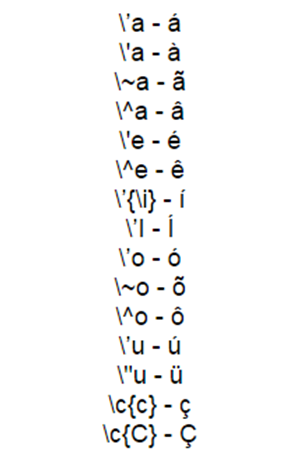
\includegraphics[scale=1.0]{USPSC-AcentuacaoLaTeX.png} \\
	Fonte: \citeonline{comandos}
	\end{center}	
\end{figure}

\chapter{Símbolos úteis em \LaTeX}
\begin{figure}[H]
	\begin{center}
		\caption{\label{fig_anexoc}Símbolos úteis em \LaTeX}
		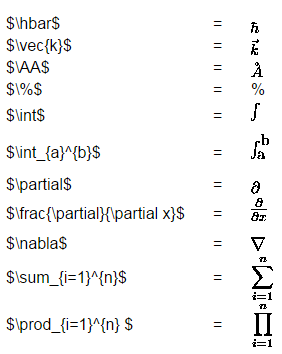
\includegraphics[scale=1.0]{USPSC-SimbolosUteis.png} \\
		Fonte: \citeonline{comandos}
	\end{center}	
\end{figure}


\chapter{Letras gregas em \LaTeX}
\begin{figure}[H]
	\begin{center}
		\caption{\label{fig_anexod}Letras gregas em \LaTeX}
		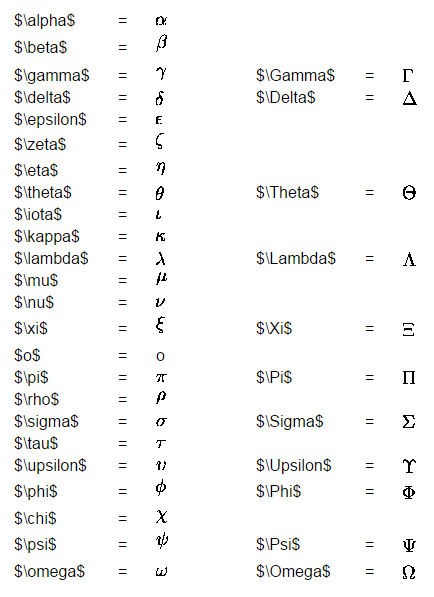
\includegraphics[scale=1.0]{USPSC-LetrasGregas.png} \\
		Fonte: \citeonline{comandos}
	\end{center}	
\end{figure}

\end{anexosenv}


%---------------------------------------------------------------------
% INDICE REMISSIVO
%--------------------------------------------------------------------
%%% USPSC-IndicexRemissivos.tex
% ---
% Inicia os Índices Remissivos
% ---
%---------------------------------------------------------------------
% INDICE REMISSIVO
%--------------------------------------------------------------------
\phantompart
\printindex
%---------------------------------------------------------------------


%---------------------------------------------------------------------

\end{document}
